\documentclass[openany,12pt,oneside]{extreport}

% ===========================
% Packages
% ===========================

% --- Core Setup for Modern LaTeX (XeLaTeX or LuaLaTeX REQUIRED) ---
\usepackage{fontspec}                % REQUIRED for \newfontfamily and modern font handling with Xe/LuaLaTeX
\usepackage{amsmath}                 % AMS Math packages
\usepackage{amsfonts}
\usepackage{amssymb}
\usepackage{amsthm}                  % For theorem-like environments (if you use them)

% Load packages that modify page layout or fundamental definitions BEFORE polyglossia/bidi
\usepackage{fancyhdr}                % Fancy headers and footers
\usepackage[Glenn]{fncychap}         % Fancy chapter headers
\usepackage{titlesec}                % Custom section titles

\usepackage{polyglossia}             % Multiple language support
\setdefaultlanguage{english}         % Set default language to English
\setotherlanguage{arabic}            % Set secondary language to Arabic
\newfontfamily\arabicfont[Script=Arabic]{Amiri} % Arabic font

% Font and Formatting
\usepackage{lmodern}                 % Latin Modern fonts
\usepackage{romannum}                % Roman numeral support
\usepackage{indentfirst}             % Indent first paragraph
\usepackage{extsizes}                % Extended sizes for fonts

% Graphics and Colors
\usepackage{graphicx}                % Enhanced graphics support
\usepackage{xcolor}  
% ===================== PACKAGES ======================
 % For \sectionfont and \subsectionfont% Enhanced color support
\usepackage{subcaption}              % Modern subfigure support
\usepackage[table]{xcolor}           % Color support for tables

% Hyperlinks
\usepackage{hyperref}                % Hyperlink support
\hypersetup{
  colorlinks = true,                 % Enable colored links
  urlcolor = black,                   % URL color
  linkcolor = black,                  % Link color
  citecolor = black                   % Citation color
}

% Tables
\usepackage{tabularx}                % Extra features for tabular environment
\usepackage{array}                   % Array and tabular environments
\usepackage{booktabs}                % Enhancements for tabular
\usepackage{multirow}                % Multi-row support
\usepackage{tabu}                    % Flexible tabular support

% Floating elements
\usepackage{float}                   % Enhanced floating support
\usepackage{wrapfig}                 % Wrap text around figures

% Captions
\usepackage{caption}                 % Customisation of captions

% Algorithm
\usepackage[ruled,vlined,linesnumbered,commentsnumbered]{algorithm2e} % <<--- ADDED THIS LINE

% Glossaries and Acronyms
\usepackage[acronym, automake]{glossaries} % Glossaries and acronyms support
\makeglossaries

% Bibliography
\usepackage[backend=biber,sorting=none]{biblatex} % Bibliography support
\addbibresource{bibliography/references.bib}      % Path to the bibliography file

% Lists
\usepackage{listofitems}             % Handling lists of items

% Diagrams and Plots
\usepackage{tikz}                    % TikZ for drawing
\usetikzlibrary{matrix,chains,positioning,decorations.pathreplacing,arrows,arrows.meta,calc}
\tikzset{>=latex}                    % Set default arrow style
\usepackage{tcolorbox}               % For colored/framed boxes, often with TikZ


% Page Layout
\usepackage[top=3cm, bottom=3cm, left=3cm, right=3cm, headheight=15pt]{geometry} % Page margins

% Chapter and Section Titles (fncychap and titlesec already loaded earlier)
\def\toclevel@subsubsubsection{4}    % Sub-sub-subsections in TOC
\def\l@subsubsubsection{\@dottedtocline{4}{7em}{4em}}
\setcounter{secnumdepth}{4}          % Numbering depth
\setcounter{tocdepth}{4}             % TOC depth

% Miscellaneous
\usepackage{pdflscape}               % Landscape support in PDF
\usepackage{footmisc}                % Footnote support
\usepackage[outline]{contour}        % Contour support for text
\contourlength{1.4pt}
\usepackage[normalem]{ulem}          % Underlining support
\usepackage{lipsum}                  % Lorem ipsum dummy text
\usepackage{bbding}                  % Dingbat symbols
\usepackage{dsfont}                  % For \mathds{1}
\usepackage{ifpdf}                   % Conditional compilation


% Document Title (usually set before \maketitle in the document body)
\title{Report_Template}

% Custom Commands
\newcommand{\challenge}[2]{
\vspace{1ex}
\textbf{Research task {#1}}: \emph{#2}
\vspace{1ex}}
\newcommand{\task}[2]{\challenge{#1}{#2}}
\newcommand{\taskref}[1]{\textbf{Task~}\ref{#1}}
\newcounter{tasknmbr}
\newcounter{tasklabel}
\renewcommand{\thetasklabel}{\textbf{\thetasknmbr}}
\newenvironment{taskenv}{
\begin{list}{\textbf{Task }\thetasklabel:}{\usecounter{tasklabel}\stepcounter{tasknmbr}\item\em}}{\\[-7pt]\end{list}} % This file should contain \usepackage{fancyhdr} and \usepackage{xcolor}
\linespread{1.5}
\setmainfont{Times New Roman}
\begin{document}

\include{FrontMatter/titlepage}
% \include{FrontMatter/Dedication} % If you have one
% % Aknowledgement
\vspace*{4cm}
\begin{center}
    {\Large \bf Acknowledgement}
\end{center} \vskip 0.5cm \vskip 0.5cm

\lipsum[1] \\
 % Moved after pagenumbering for consistency if these have the style
% % Abstract
\vspace*{4cm}
\begin{center}
    {\Large\bf Abstract}
\end{center} \vskip 0.5cm \vskip 0.5cm
\lipsum[1] \\

\providecommand{\keywords}[1] {
  \small	
  \textbf{\textit{Keywords---}} #1
}
\keywords{keyword 1, keyword 2}

% \chapter{Acronyms}

% Reduce spacing between rows and overall text size



% Tighter row spacing
\renewcommand{\arraystretch}{0.9}  % Default is 1.0

% Set smaller font and remove extra vertical spacing before/after longtable
\vspace*{-1em}
{\footnotesize  % smaller than \small

\setlength{\LTleft}{0pt}
\setlength{\LTright}{0pt}

% General & Security Terms Table
\begin{longtable}{|>{\bfseries}p{2.5cm}|>{\raggedright\arraybackslash}p{8.5cm}|}
\hline
\multicolumn{2}{|c|}{\textbf{General \& Security Terms (A-Z)}} \\
\hline
API & Application Programming Interface \\
AWS EC2 & Amazon Web Services Elastic Compute Cloud \\
CA & Certificate Authority \\
CCPA & California Consumer Privacy Act \\
CN & Common Name (in certificates) \\
CSS & Cascading Style Sheets \\
CSV & Comma-Separated Values \\
HTTPS & Hypertext Transfer Protocol Secure \\
IP & Internet Protocol \\
IoT & Internet of Things \\
JWT & JSON Web Token \\
LoRa & Long Range (radio communication) \\
LoRaWAN & LoRa Wide Area Network \\
mTLS & mutual Transport Layer Security \\
PIPEDA & Personal Information Protection and Electronic Documents Act \\
SMPC & Secure Multi-Party Computation \\
SMS & Short Message Service \\
SQLite & A database engine \\
TLS & Transport Layer Security \\
ZIP & An archive file format \\
\hline
\end{longtable}

\vspace*{-1em}  % reduce space between tables

% ML / Technical Terms Table
\begin{longtable}{|>{\bfseries}p{2.5cm}|>{\raggedright\arraybackslash}p{8.5cm}|}
\hline
\multicolumn{2}{|c|}{\textbf{ML / Technical Terms (A-Z)}} \\
\hline
CFL & Centralized Federated Learning \\
CNNs & Convolutional Neural Networks \\
DB1, DB2 & Labels for databases \\
DFL & Decentralized Federated Learning \\
DO & Dissolved Oxygen \\
E2E & End-to-End (testing) \\
ESP32 & A type of microcontroller \\
FedAvg & Federated Averaging \\
FL & Federated Learning \\
FTL & Federated Transfer Learning \\
HFL & Heterogeneous/Horizontal Federated Learning \\
IQR & Interquartile Range \\
KD & Knowledge Distillation \\
KNN & K-Nearest Neighbors \\
MAE & Mean Absolute Error \\
MCN-LSTM & Multivariate CNN with Long Short-Term Memory \\
ML & Machine Learning \\
NaN & Not a Number \\
non-IID & Non-independent and identically distributed \\
Pytest & A Python testing framework \\
R2 & R-squared (coefficient of determination) \\
RAM & Random Access Memory \\
ReLU & Rectified Linear Unit \\
RMSE & Root Mean Square Error \\
RNN & Recurrent Neural Network \\
SimpleRNN & Simple Recurrent Neural Network \\
SVM & Support Vector Machine \\
VFL & Vertical Federated Learning \\
Vitest & A Vite-based testing framework \\
WQI & Water Quality Index \\
WQM & Water Quality Monitoring \\
\hline
\end{longtable}

} % end of \footnotesize

\vspace*{-1em}
\pagebreak


% \pagenumbering{roman} % For front matter if you want roman numerals
% ... (your front matter includes that should have roman numbering or no numbering)

\cleardoublepage % Ensures new page style starts correctly if switching numbering
\pagenumbering{arabic} % Switch to Arabic numbering for main content

% Define colors (if not already in packages.tex, but good to have them accessible)
\definecolor{myheaderfooterlinecolor}{rgb}{0.0, 0.0, 0.55} % A nice blue, adjust as needed
\definecolor{darkblue}{rgb}{0.0, 0.0, 0.55}
\definecolor{darkgreen}{rgb}{0.0, 0.5, 0.0} % Adjusted for better visibility than 0.39

% --- Fancy Header/Footer Setup for Main Chapters ---
\fancypagestyle{mainchapterstyle}{%
    \fancyhf{} % Clear all header and footer fields
    \renewcommand{\headrulewidth}{0.4pt} % Thickness of the header rule
    \renewcommand{\footrulewidth}{0.4pt} % Thickness of the footer rule
    \fancyhead[L]{\small\textcolor{myheaderfooterlinecolor}{\leftmark}} % Chapter name on the left
    % \fancyhead[C]{} % Center header empty
    % \fancyhead[R]{} % Right header empty

     % Your name on the left
    \fancyfoot[C]{\small\textcolor{myheaderfooterlinecolor}{\thepage}} % Page number in the center
    \fancyfoot[R]{\small\textcolor{myheaderfooterlinecolor}{2024/2025}} % Academic year on the right
    % Adjust colors and text as needed
}
\pagestyle{mainchapterstyle} % Apply this style to subsequent pages

%
% Section numbering (keep your existing definitions)
\renewcommand{\thesection}{\Roman{section}}
\renewcommand{\thesubsection}{\hspace*{0.1cm} \arabic{subsection}}
\renewcommand{\thesubsubsection}{\hspace*{0.2cm} \arabic{subsection}.\arabic{subsubsection}}
% Customize section titles (keep your existing definitions)
\titleformat{\section}
  {\normalfont\Large\bfseries\color{darkblue}}
  {\thesection}
  {1em}
  {}
\titleformat{\subsection}
  {\normalfont\large\bfseries\color{darkgreen}}
  {\thesubsection}
  {1em}
  {}

% --- Include your content ---
% These should now have the 'mainchapterstyle'
\newpage % Good practice before starting main content after style changes
% Aknowledgement
\vspace*{4cm}
\begin{center}
    {\Large \bf Acknowledgement}
\end{center} \vskip 0.5cm \vskip 0.5cm

\lipsum[1] \\
 % If these should also have the main style
% Abstract
\vspace*{4cm}
\begin{center}
    {\Large\bf Abstract}
\end{center} \vskip 0.5cm \vskip 0.5cm
\lipsum[1] \\

\providecommand{\keywords}[1] {
  \small	
  \textbf{\textit{Keywords---}} #1
}
\keywords{keyword 1, keyword 2}

\chapter{Acronyms}

% Reduce spacing between rows and overall text size



% Tighter row spacing
\renewcommand{\arraystretch}{0.9}  % Default is 1.0

% Set smaller font and remove extra vertical spacing before/after longtable
\vspace*{-1em}
{\footnotesize  % smaller than \small

\setlength{\LTleft}{0pt}
\setlength{\LTright}{0pt}

% General & Security Terms Table
\begin{longtable}{|>{\bfseries}p{2.5cm}|>{\raggedright\arraybackslash}p{8.5cm}|}
\hline
\multicolumn{2}{|c|}{\textbf{General \& Security Terms (A-Z)}} \\
\hline
API & Application Programming Interface \\
AWS EC2 & Amazon Web Services Elastic Compute Cloud \\
CA & Certificate Authority \\
CCPA & California Consumer Privacy Act \\
CN & Common Name (in certificates) \\
CSS & Cascading Style Sheets \\
CSV & Comma-Separated Values \\
HTTPS & Hypertext Transfer Protocol Secure \\
IP & Internet Protocol \\
IoT & Internet of Things \\
JWT & JSON Web Token \\
LoRa & Long Range (radio communication) \\
LoRaWAN & LoRa Wide Area Network \\
mTLS & mutual Transport Layer Security \\
PIPEDA & Personal Information Protection and Electronic Documents Act \\
SMPC & Secure Multi-Party Computation \\
SMS & Short Message Service \\
SQLite & A database engine \\
TLS & Transport Layer Security \\
ZIP & An archive file format \\
\hline
\end{longtable}

\vspace*{-1em}  % reduce space between tables

% ML / Technical Terms Table
\begin{longtable}{|>{\bfseries}p{2.5cm}|>{\raggedright\arraybackslash}p{8.5cm}|}
\hline
\multicolumn{2}{|c|}{\textbf{ML / Technical Terms (A-Z)}} \\
\hline
CFL & Centralized Federated Learning \\
CNNs & Convolutional Neural Networks \\
DB1, DB2 & Labels for databases \\
DFL & Decentralized Federated Learning \\
DO & Dissolved Oxygen \\
E2E & End-to-End (testing) \\
ESP32 & A type of microcontroller \\
FedAvg & Federated Averaging \\
FL & Federated Learning \\
FTL & Federated Transfer Learning \\
HFL & Heterogeneous/Horizontal Federated Learning \\
IQR & Interquartile Range \\
KD & Knowledge Distillation \\
KNN & K-Nearest Neighbors \\
MAE & Mean Absolute Error \\
MCN-LSTM & Multivariate CNN with Long Short-Term Memory \\
ML & Machine Learning \\
NaN & Not a Number \\
non-IID & Non-independent and identically distributed \\
Pytest & A Python testing framework \\
R2 & R-squared (coefficient of determination) \\
RAM & Random Access Memory \\
ReLU & Rectified Linear Unit \\
RMSE & Root Mean Square Error \\
RNN & Recurrent Neural Network \\
SimpleRNN & Simple Recurrent Neural Network \\
SVM & Support Vector Machine \\
VFL & Vertical Federated Learning \\
Vitest & A Vite-based testing framework \\
WQI & Water Quality Index \\
WQM & Water Quality Monitoring \\
\hline
\end{longtable}

} % end of \footnotesize

\vspace*{-1em}
\pagebreak

\newpage

\tableofcontents
\listoffigures
\listoftables
% \printglossary[type=\acronymtype, title=Acronyms] % You already have \chapter{Acronyms}

% Reduce spacing between rows and overall text size



% Tighter row spacing
\renewcommand{\arraystretch}{0.9}  % Default is 1.0

% Set smaller font and remove extra vertical spacing before/after longtable
\vspace*{-1em}
{\footnotesize  % smaller than \small

\setlength{\LTleft}{0pt}
\setlength{\LTright}{0pt}

% General & Security Terms Table
\begin{longtable}{|>{\bfseries}p{2.5cm}|>{\raggedright\arraybackslash}p{8.5cm}|}
\hline
\multicolumn{2}{|c|}{\textbf{General \& Security Terms (A-Z)}} \\
\hline
API & Application Programming Interface \\
AWS EC2 & Amazon Web Services Elastic Compute Cloud \\
CA & Certificate Authority \\
CCPA & California Consumer Privacy Act \\
CN & Common Name (in certificates) \\
CSS & Cascading Style Sheets \\
CSV & Comma-Separated Values \\
HTTPS & Hypertext Transfer Protocol Secure \\
IP & Internet Protocol \\
IoT & Internet of Things \\
JWT & JSON Web Token \\
LoRa & Long Range (radio communication) \\
LoRaWAN & LoRa Wide Area Network \\
mTLS & mutual Transport Layer Security \\
PIPEDA & Personal Information Protection and Electronic Documents Act \\
SMPC & Secure Multi-Party Computation \\
SMS & Short Message Service \\
SQLite & A database engine \\
TLS & Transport Layer Security \\
ZIP & An archive file format \\
\hline
\end{longtable}

\vspace*{-1em}  % reduce space between tables

% ML / Technical Terms Table
\begin{longtable}{|>{\bfseries}p{2.5cm}|>{\raggedright\arraybackslash}p{8.5cm}|}
\hline
\multicolumn{2}{|c|}{\textbf{ML / Technical Terms (A-Z)}} \\
\hline
CFL & Centralized Federated Learning \\
CNNs & Convolutional Neural Networks \\
DB1, DB2 & Labels for databases \\
DFL & Decentralized Federated Learning \\
DO & Dissolved Oxygen \\
E2E & End-to-End (testing) \\
ESP32 & A type of microcontroller \\
FedAvg & Federated Averaging \\
FL & Federated Learning \\
FTL & Federated Transfer Learning \\
HFL & Heterogeneous/Horizontal Federated Learning \\
IQR & Interquartile Range \\
KD & Knowledge Distillation \\
KNN & K-Nearest Neighbors \\
MAE & Mean Absolute Error \\
MCN-LSTM & Multivariate CNN with Long Short-Term Memory \\
ML & Machine Learning \\
NaN & Not a Number \\
non-IID & Non-independent and identically distributed \\
Pytest & A Python testing framework \\
R2 & R-squared (coefficient of determination) \\
RAM & Random Access Memory \\
ReLU & Rectified Linear Unit \\
RMSE & Root Mean Square Error \\
RNN & Recurrent Neural Network \\
SimpleRNN & Simple Recurrent Neural Network \\
SVM & Support Vector Machine \\
VFL & Vertical Federated Learning \\
Vitest & A Vite-based testing framework \\
WQI & Water Quality Index \\
WQM & Water Quality Monitoring \\
\hline
\end{longtable}

} % end of \footnotesize

\vspace*{-1em}
\pagebreak

                                                  % Choose one way to include acronyms.
                                                  % If Acronyms.tex uses \printglossary, then this is fine.
                                                  % Otherwise, if Acronyms.tex is just text, remove this \printglossary.
\clearpage


\include{Chapters/01_Introduction}
% \newcommand{\RomanNumeralCaps}[1]{\MakeUppercase{\romannum{#1}}.}
\chapter{General Project Context}
\label{chap: General Project Context}

\section*{Introduction}

This chapter provides a general overview of the host company, presenting its background, including its history and its current positioning in the market. It outlines the company’s areas of expertise, core mission, and vision. Additionally, the chapter introduces the project assigned during the internship, detailing its context, the problem it aims to address, and the proposed solution. It also presents the project brief, defining the functional and technical specifications of the project. Finally, this chapter highlights the project management methodology adopted  such as the Agile approach  and includes a Gantt chart to illustrate the planning and distribution of tasks over time.

\newpage

\phantomsection
\addcontentsline{toc}{section}{Presentation of Host Organization}
\section{Presentation of Host Organization}

 \subsection{History and Positioning}
 \begin{figure}[H] 
    \centering
    
\includegraphics[width=5cm]{Logos/Company_Logo.png}
    \caption{Company logo}
    %\label{fig:my_label} %Optional (If you want to reference the figure in later chapters)
\end{figure}

Founded in 2017 in Tétouan, Yafa Technologies is a Moroccan company located at 11, Avenue Zerktouni, Appart 12, Tétouan 93000. Since its creation, the company has steadily grown and established itself as a recognized player in the field of custom IT solutions and digital transformation services.

Through its commitment to innovation and quality, Yafa Technologies has built a strong reputation by responding effectively to the specific needs of both private companies and public institutions. Its strategic positioning focuses on developing tailored digital tools that help clients optimize their operations, improve productivity, and embrace technological change
    \subsection{Mission and Vision}

Yafa Technologies' mission is to provide reliable and secure IT solutions that support its clients in improving their operations and staying competitive. Its vision is to be a trusted partner in digital transformation, helping organizations make better decisions through the use of modern technologies and practical expertise..
    \subsection{ Areas of Expertise}

 Yafa Technologies offers a comprehensive suite of services, demonstrating its versatility and commitment to holistic client support. These include:
    \begin{itemize}
        \item \textbf{Custom Software Development:} Designing and implementing bespoke software applications tailored to specific business requirements.
        \item \textbf{Web and Mobile Application Development:} Creating intuitive and powerful applications to enhance user engagement and operational efficiency.
        \item \textbf{Data Analytics and Business Intelligence:} Providing solutions for data collection, processing, analysis, and visualization to derive actionable insights.
        \item \textbf{Cloud Computing Solutions:} Assisting organizations in migrating to and managing cloud infrastructure for enhanced scalability and flexibility.
        \item \textbf{IT Consulting and Professional Training:} Offering expert advice and customized training programs to build internal capacity and optimize IT strategies.
        \item \textbf{Cybersecurity Services:} Implementing robust security measures to protect digital assets and ensure data integrity.
    \end{itemize}









\subsection{Organizational Chart}

\begin{figure}[H] 
    \centering
    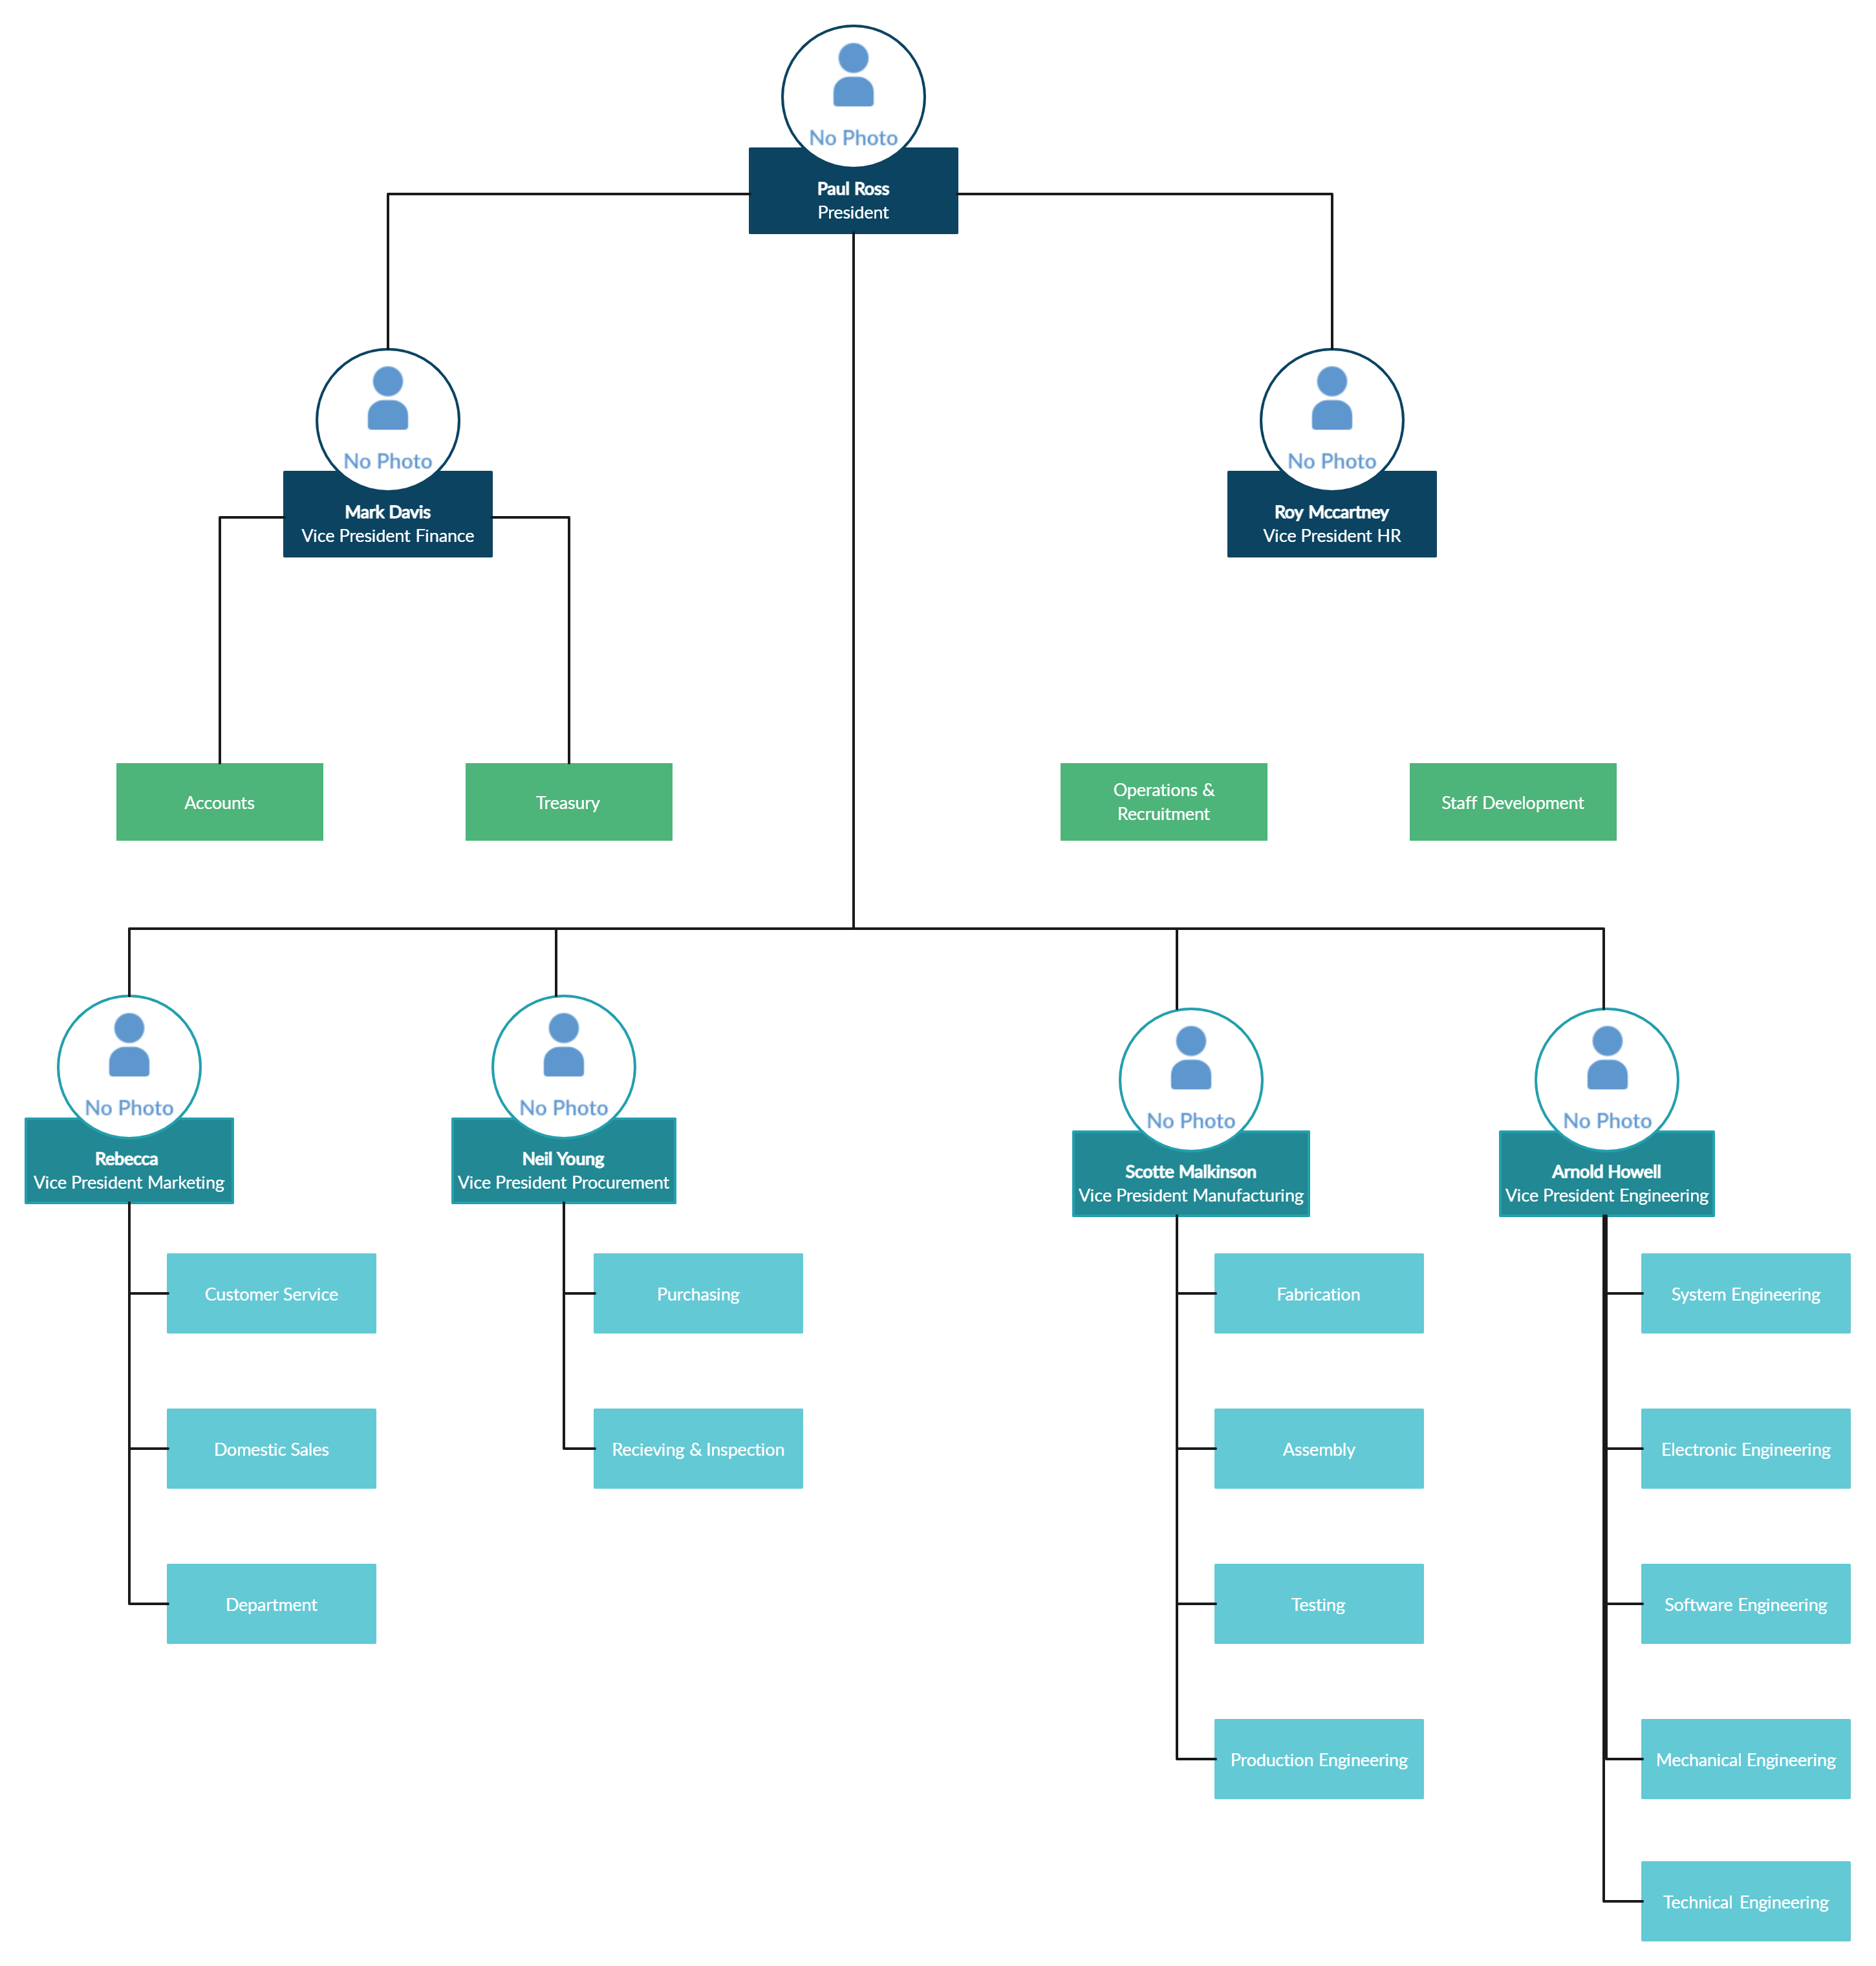
\includegraphics[width=1cm]{Figures/Organizational_Chart.png}
    \caption{Organizational Chart}
    %\label{fig:my_label} %Optional (If you want to reference the figure in later chapters)
\end{figure}


\section{Project Presentation}
\subsection{Topic Overview}


The main challenge of this project is to develop a comprehensive Federated Learning system that combines multiple key functions into a single platform. This system will enable the collaborative training of a time series model to predict the Water Quality Index (WQI) based on data collected from distributed sensors, all while maintaining data privacy by avoiding centralization of raw data. In addition to the model training process, the system will provide an administrative dashboard allowing authorized users to configure system parameters, monitor real-time performance metrics, and receive alerts in case of operational issues or anomalies. 

\subsection{Problematic}

 Traditional centralized approaches to water quality monitoring face several critical challenges:
    \begin{itemize}
        \item \textbf{Data Privacy:} Transmitting raw sensor data from multiple locations to a central server can raise significant privacy concerns, especially if data originates from private properties or regulated areas.
        \item \textbf{Communication Overhead:} Continuously streaming large volumes of sensor data can be bandwidth-intensive and costly, particularly in remote areas with limited connectivity.
        \item \textbf{Scalability:} Centralized systems can struggle to scale efficiently as the number of monitoring points increases, leading to bottlenecks in data processing and storage.
        \item \textbf{Latency:} Relying on cloud processing can introduce delays in detecting critical water quality issues, hindering rapid response.
        \item \textbf{Single Point of Failure:} A centralized server represents a single point of failure; if it goes down, the entire monitoring system can be compromised.
    \end{itemize}

% \subsection{Specifications document}

% TODO:

\subsection{Project Management}
\subsubsection{Agile Practices}
To allow flexibility and responsiveness during the process of creating the Federating Learning Project, Agile methods are incorporated into the process. The project is structured in phases with activities and milestones well-defined so that iterative improvements and continuous feedback incorporation can be accomplished. Each phase, from Formation and Study to Testing and Reporting, consists of an incremental development cycle, wherein the system progressively develops and fixes potential issues early in the process.

Agile methodology is observed through task dependency and concurrent processes in the project. For example, during the Environment Setup stage, certain of the preparatory tasks of Core Development can run in parallel to enable effective usage of resources. Ongoing teamwork and sprint planning allow for bottleneck detection and prioritization of the work to be done so that every development iteration contains a workable and testable component.

Moreover, Agile patterns such as frequent testing and validation are implemented, primarily during the Testing \& Reporting phase. Through continuous testing of the federated learning convergence of the system and security enhancement, feedback loops are established to enhance encryption processes and optimize model performance. Documentation refreshes at key points are also embraced by the project, with the PFE adapting in line with development and minimizing technical debt while optimizing knowledge transfer.

Using the Agile principles, the Federating Learning Project maintains responsiveness to changing needs, streamlines collaboration, and ensures delivery meets both the technical and business expectations.

\subsubsection{Internship Planning}
\begin{figure}[H]
    \centering
    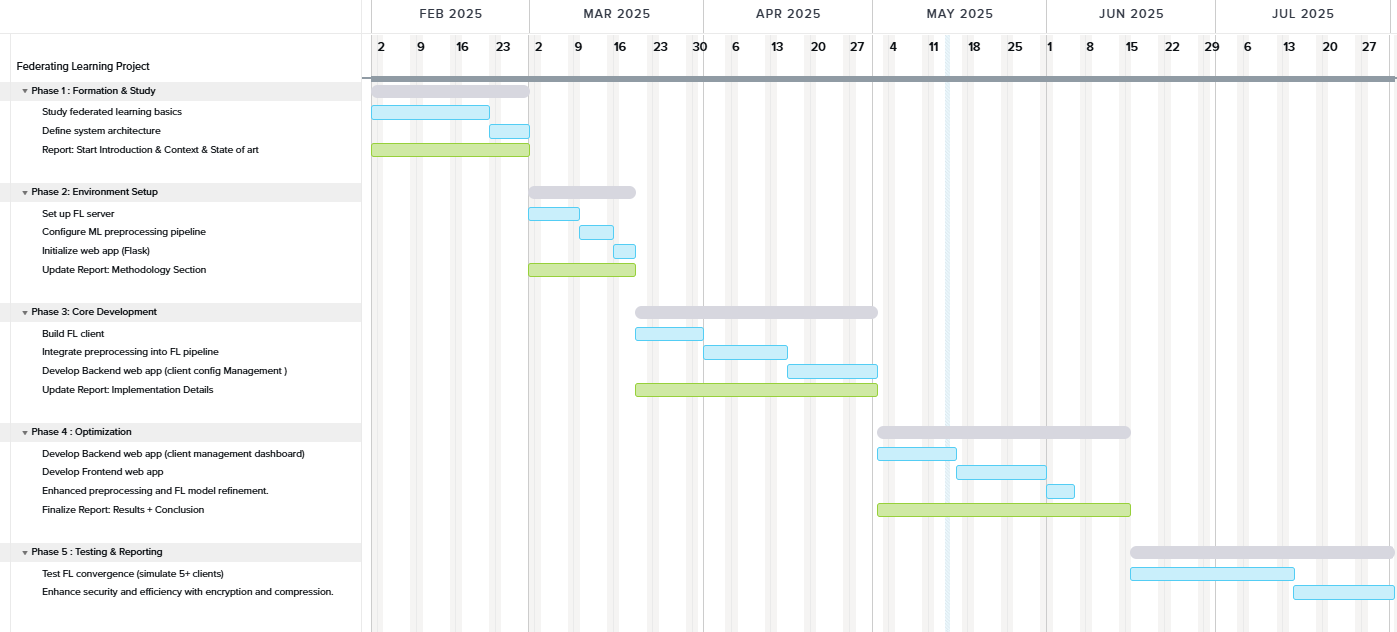
\includegraphics[width=1\linewidth]{Figures/Gantt.png}
    \caption{Gantt Diagram}
    \label{fig:enter-label}
\end{figure}
The Federating Learning Project follows a phased and systematic process to carry out a smooth and effective development. The project is started with Phase 1: Formation and Study, in which it is planned to acquire initial knowledge about federated learning, defining the structure of the system, and establishing the context and state of the art for Report. This phase ensures a clear understanding of the objectives, methodologies, and technological requirements before moving ahead. Following the initial study, Phase 2: Environment Setup is devoted to the installation of the necessary infrastructure. This involves the installation of the federated learning server, machine learning preprocessing pipeline configuration, and web application initialization with Flask. The Report methodology section is also updated to include these advances, with proper documentation of the installation phase.

Once the environment is set up, the project proceeds to Phase 3: Core Development, where the core components of the system are built. This phase includes building the FL client, implementing preprocessing in the federated learning pipeline, and building the backend web app for client configuration management. During this phase, the implementation details of the Report are also updated to track progress.

The Optimization Phase (Phase 4) is used to enhance and refine the system.

The backend web application is enhanced to include a client management dashboard, a frontend web application is developed, and additional enhancements are made to the preprocessing and federated learning model. The system is fully functional, efficient, and user-friendly in this phase. Besides, the Results and Conclusion of the Report is finalized, such as knowledge and experience gained in the development and optimization process. Phase 5: Testing and Reporting, the final phase, is crucial in confirming the functionality and security of the system. Convergence of federated learning is tested through simulations involving at least five clients to examine its performance. Additionally, security patches by way of encryption and compression techniques are incorporated to determine data confidentiality and integrity. Every step of the project is carefully planned and executed sequentially with dependencies between tasks to produce a logical progression. This methodical approach guarantees effective and well-documented development, leading to the successful deployment of a federated learning system.

\newpage

\section*{Conclusion}

% \chapter{State of Art}
\label{chap:Chapter 2 title}
\section*{Introduction}

Traditionally, machine learning (ML) has relied on centralized approaches, where models are trained on powerful servers using large, aggregated datasets. Although the centralized paradigm remains prevalent, emerging decentralized approaches, such as edge computing and federated learning, are gaining traction to address specific limitations. In centralized training, aggregating large amounts of data from multiple sources raises concerns about privacy, security, and latency. This is particularly critical under data protection regulations such as the GDPR (Europe), CCPA (California), and PIPEDA (Canada) etc., which restrict the transfer and centralized storage of sensitive personal data.

With the proliferation of devices on the Internet of Things (IoT) and the exponential growth of data generation, there is a growing need for scalable solutions capable of processing data locally. Edge computing addresses this need by enabling data processing at or near the data source, thus reducing latency and alleviating bandwidth demands. Building upon edge computing, federated learning (FL) enables the collaborative training of ML models across decentralized devices, each retaining its local data, thus avoiding the need to transmit raw data. This paradigm improves privacy while leveraging the computational capabilities of edge devices, making it suitable for applications where data sensitivity and real-time processing are paramount \cite{ref1}.

A core challenge in this decentralized paradigm lies in building robust models across heterogeneous devices without centralizing sensitive data. Devices in a federated learning setup often differ in computational resources, storage capacity, and network stability, complicating synchronization and model aggregation. Furthermore, data across devices are frequently nonindependent and identically distributed (non-IID), leading to biases that can negatively impact model performance. To address these challenges, researchers have proposed various strategies, including adapting model architectures for heterogeneous environments and designing aggregation algorithms that ensure fair and efficient training. However, achieving optimal performance in federated learning remains an open research question, with ongoing work aimed at balancing privacy, model accuracy, and system efficiency \cite{ref2}.


\pagebreak


\section{Federated learning}

Federated Learning (FL) is revolutionizing machine learning by enabling decentralized modeling while preserving data privacy. Unlike traditional approaches that aggregate raw data into centralized servers, FL distributes a pre-trained global model to edge devices  such as smartphones, IoT sensors, and even low-cost hardware like Raspberry Pis  which then perform local training using their private data. This decentralized paradigm not only addresses privacy and regulatory concerns (e.g., GDPR compliance) but also reduces communication overhead, making it well-suited for dynamic and resource-constrained environments.

% \section{Evolution of Federated Learning (FL)}
% \subsection{Foundations}
% The development of Federated Learning began with pioneering approaches that emphasized privacy preservation and efficiency:

% \begin{itemize}
%     \item	\textbf{Google’s Federated Averaging (FedAvg) (2016):}
%      FedAvg introduced a novel way to train global models by iteratively aggregating locally computed updates (e.g., weights or gradients). In this process, each device trains the model using its private dataset and sends only the updated parameters to a central server. The central server then computes a weighted average of these updates to refine the global model. This method demonstrated that robust machine learning models could be built without transferring raw, sensitive data [1], [3].
    
%     \item	\textbf{IBM’s Federated Analytics (2018):}
%      Building on the FedAvg concept, IBM’s Federated Analytics extended FL to statistical analysis tasks. By integrating early privacy-preserving techniques such as secure multi-party computation (SMPC) and differential privacy, IBM’s approach ensured that data remained local while still enabling meaningful analytics. This innovation was especially significant for industries with stringent data privacy requirements, such as healthcare and environmental monitoring [1], [8].
% \end{itemize}
% \subsection{ Breakthroughs (2019–2023)}
% Recent years have witnessed rapid advancements in Federated Learning, addressing key challenges related to scale, heterogeneity, and model convergence:

% \begin{itemize}
%     \item Cross-Device FL: Scaling to Millions of Edge Devices initially limited to a few participants, FL has evolved to support large-scale deployments. Enhanced communication protocols, bandwidth optimization, and efficient model compression have enabled millions of devices  including smartphones and IoT sensors  to participate in FL. A notable example is Google's implementation in Gboard, their mobile keyboard app, which uses federated learning to enhance next-word predictions by learning from user interactions directly on their devices, ensuring personal data remains private. [Federated Learning: Collaborative Machine Learning without Centralized Training].
%     \item Heterogeneous Federated Learning (HFL): Supporting Diverse Hardware
%      Practical FL applications must account for the diversity of edge devices. Heterogeneous FL (HFL) addresses disparities in hardware capabilities by employing strategies such as:

%     \begin{itemize}
%         \item Model Compression: Techniques such as quantization and pruning reduce the model size, enabling participation from devices with limited computational power (e.g., Raspberry Pi models ranging from 1B to 5).
%         \item Knowledge Distillation (KD): Techniques in HFL enable diverse model architectures to collaborate by exchanging distilled information (e.g., logits, features) instead of full model parameters. This approach preserves model heterogeneity while ensuring effective knowledge transfer, bridging differences in model size and complexity. [arXiv:2312.12091v2]
%     \end{itemize}
    
%      \begin{figure}[H]
%          \centering
%          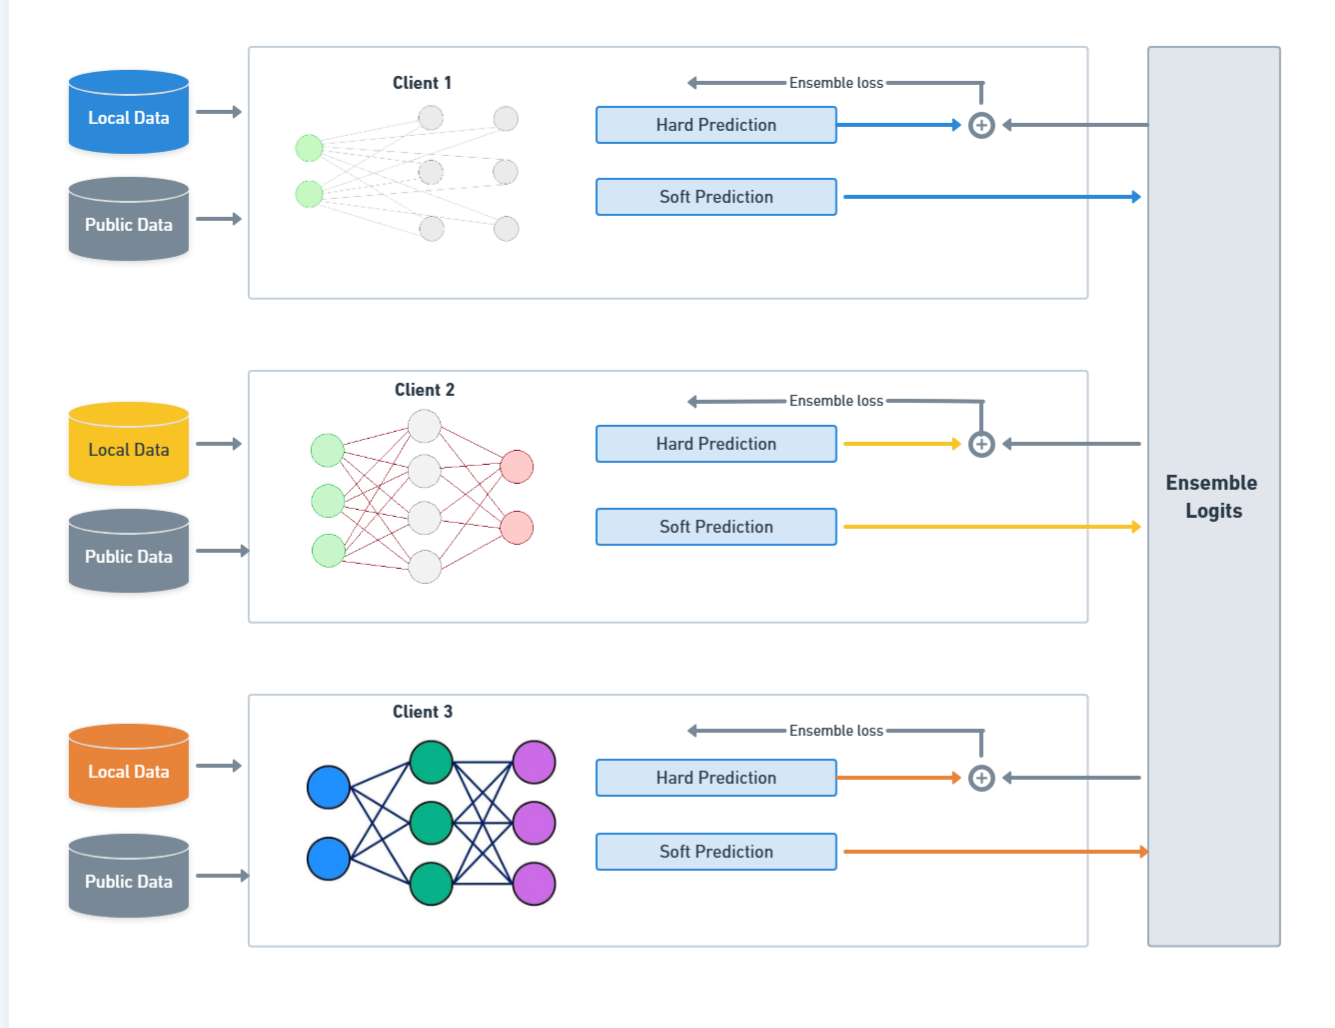
\includegraphics[width=0.75\linewidth]{Figures/KD.png}
%          \caption{Knowledge distillation}
%          \label{fig:enter-label}
%      \end{figure}

%     \begin{itemize}
        
%         \item Partial Training: Rather than training full models, devices may update only select layers, thereby lowering computational requirements while still contributing effectively to the global model. [arXiv:2312.12091v2]
        
%     \end{itemize}
%     \begin{figure}[H]
%         \centering
%         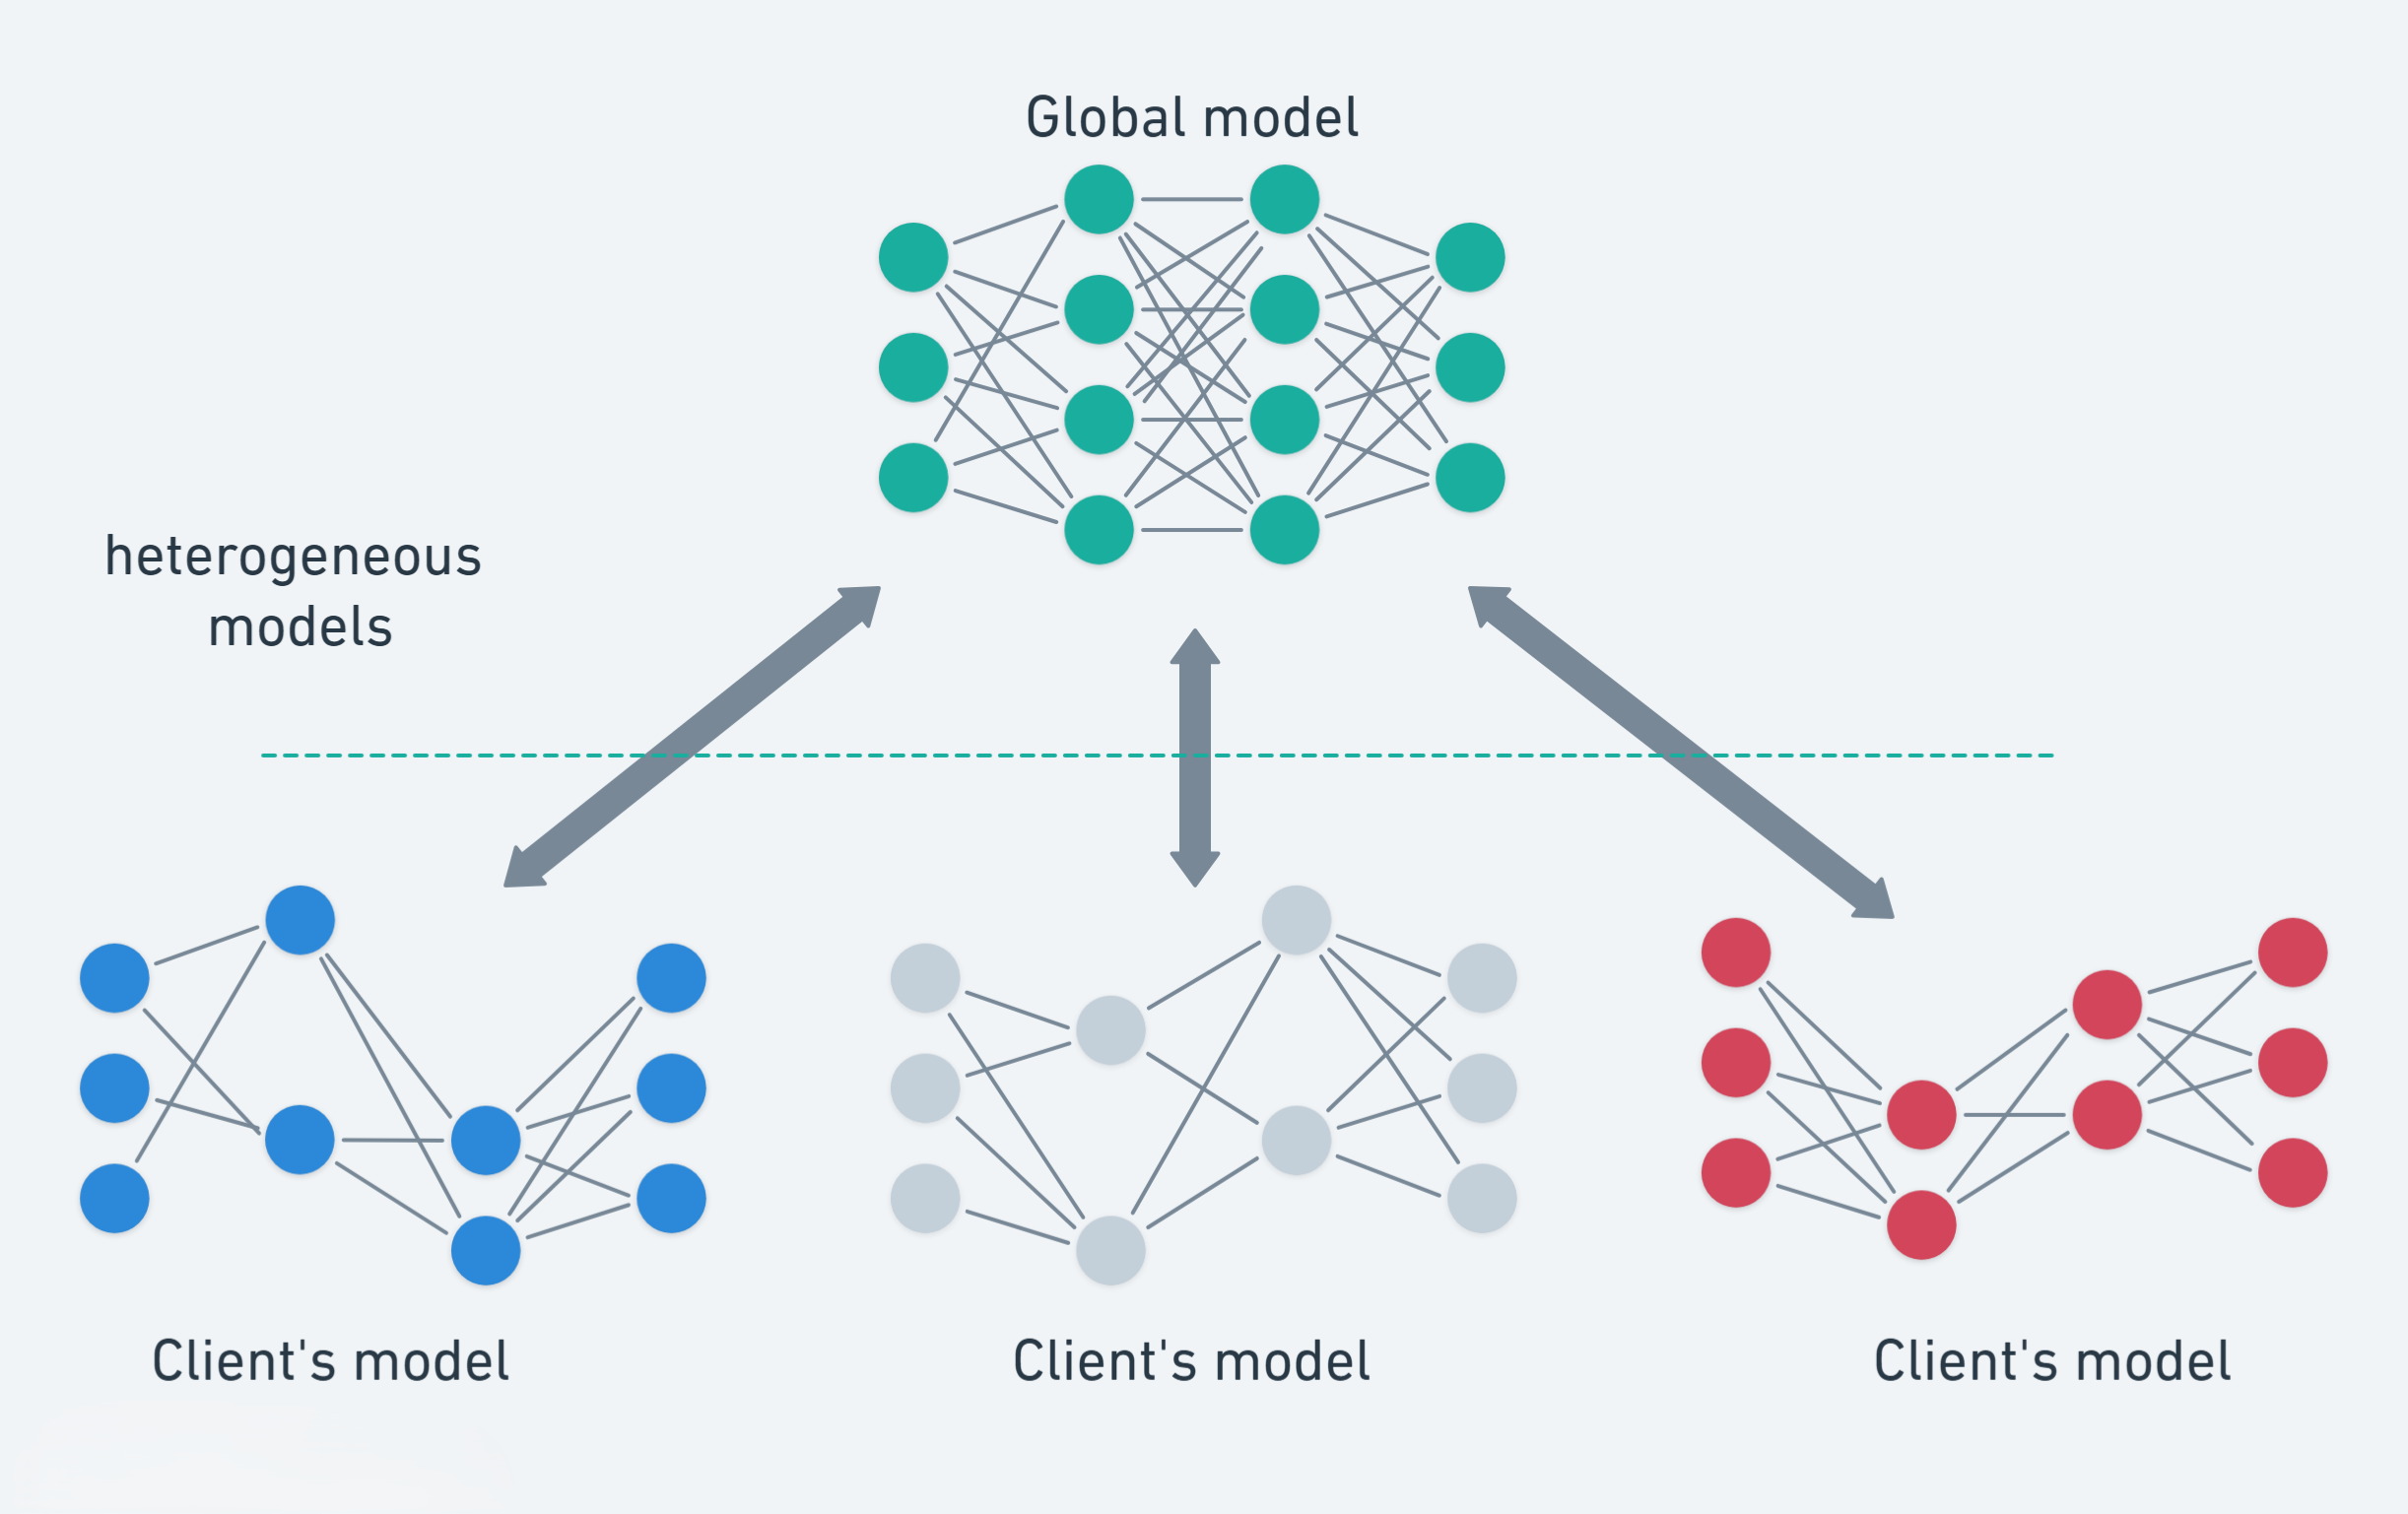
\includegraphics[width=0.5\linewidth]{Figures/partial_training.png}
%         \caption{partial training }
%         \label{fig:enter-label}
%     \end{figure}

%     \item Adaptive Aggregation: Enhancing Model Convergence
%     A persistent challenge in FL is the heterogeneity of data distributions (non-IID data) across devices, which can hinder model convergence. Recent advances include:

%     \begin{itemize}
%         \item \textbf{FedProx:} Incorporates a proximal term during local training to reduce the deviation from the global model, thereby stabilizing the training process.
%         \item \textbf{FedRolex:} A framework that enhances heterogeneous model training by using a rolling sub-model extraction method. It dynamically extracts and trains different sub-models over time, ensuring uniform training across the global model and mitigating client drift.
%         \item \textbf{SCAFFOLD:} Utilizes control variates to correct for client drift, thus mitigating the effect of local updates that might otherwise skew the global model.
%         \item \textbf{Dynamic Client Weighting:} Adjusts the contribution of each client's update according to data quality and size, ensuring that the aggregation process is balanced and robust.
%     \end{itemize}
% \end{itemize}

% These adaptive aggregation strategies have significantly improved FL performance and reliability in heterogeneous environments [2302.11466v2.pdf, arXiv:2312.12091v2].
\section{Types of Federated Learning}
\subsection{Based on Data Distribution}

\subsubsection{Horizontal Federated Learning (HFL)}
\begin{figure}[H]
    \centering
    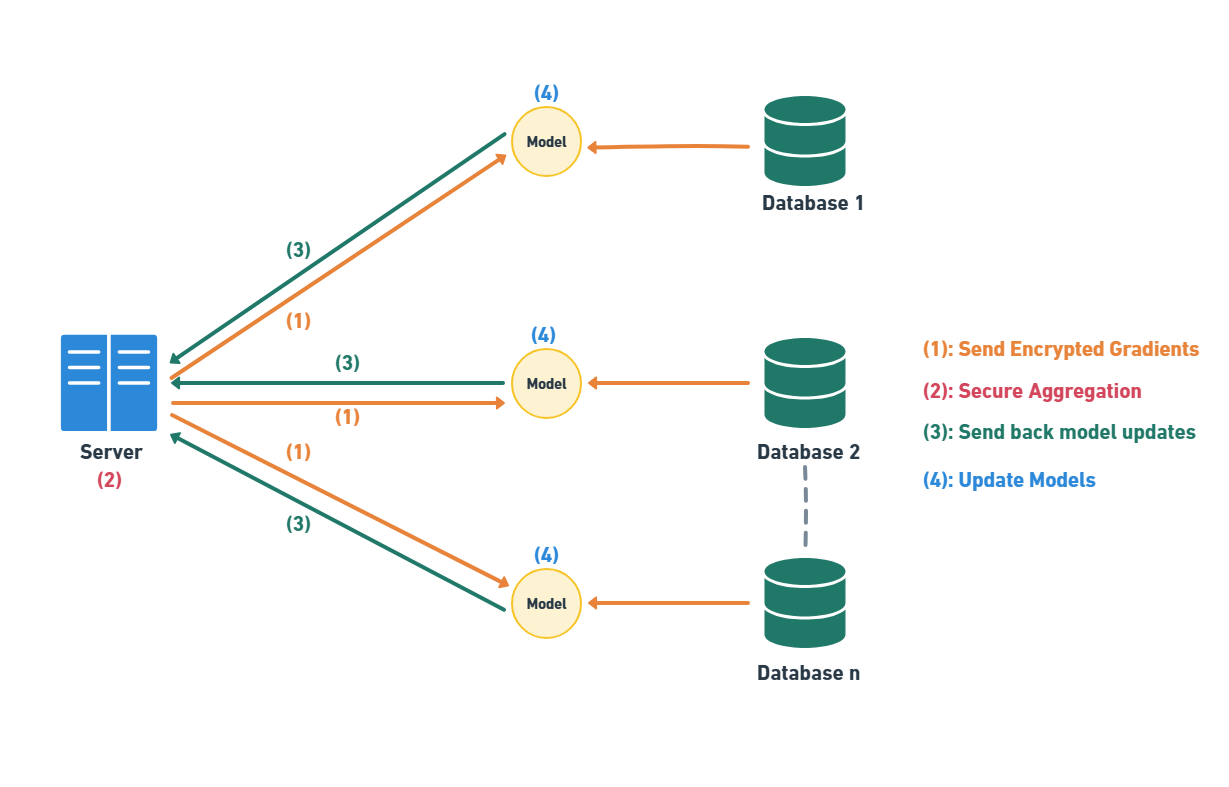
\includegraphics[width=0.75\linewidth]{Figures/diagram 1 (2).png}
    \caption{Horizontal Federated Learning}
    \label{fig:enter-label}
\end{figure}

Horizontal Federated Learning (HFL) is a decentralized machine learning approach in which multiple participants collaboratively train a shared global model without exchanging raw data. Each participant holds datasets with the same feature space, such as hospitals collecting identical health metrics, but with different data samples, ensuring both data privacy and compliance with protection regulations.




\subsubsection{Vertical Federated Learning (VFL)}
\begin{figure}[H]
    \centering
    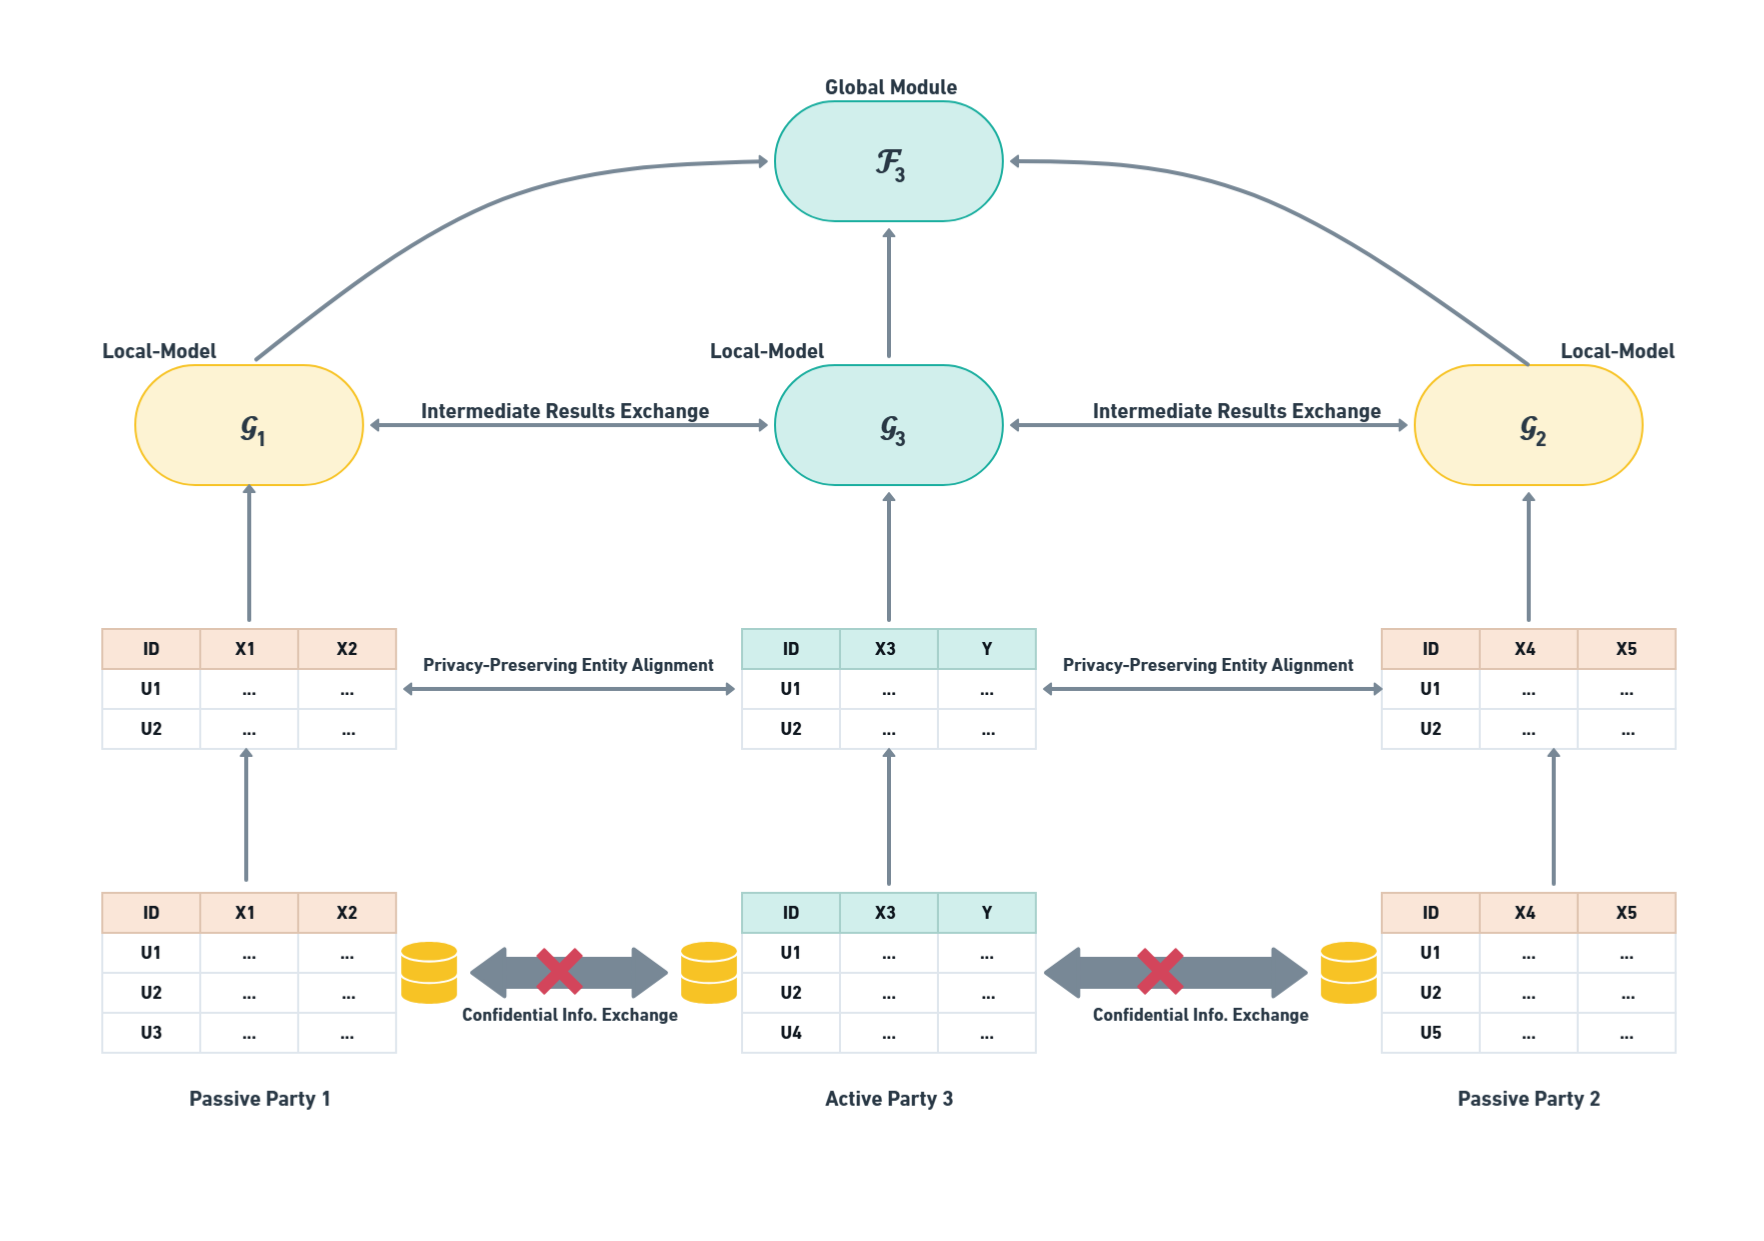
\includegraphics[width=0.75\linewidth]{Figures/VFL.png}
    \caption{Vertical Federated Learning}
    \label{fig:enter-label}
\end{figure}

Vertical Federated Learning (VFL) is tailored for scenarios where different organizations possess complementary features about the same individuals. For example, a bank can have access to a customer’s financial records, while a retailer holds their purchase history. By collaborating, these entities can train a more comprehensive model without revealing their raw data. In VFL, the feature space is partitioned, which means that each participant has a distinct subset of features for the same set of users,





\section{Based On Network Structure}

\begin{figure}[H]
    \centering
    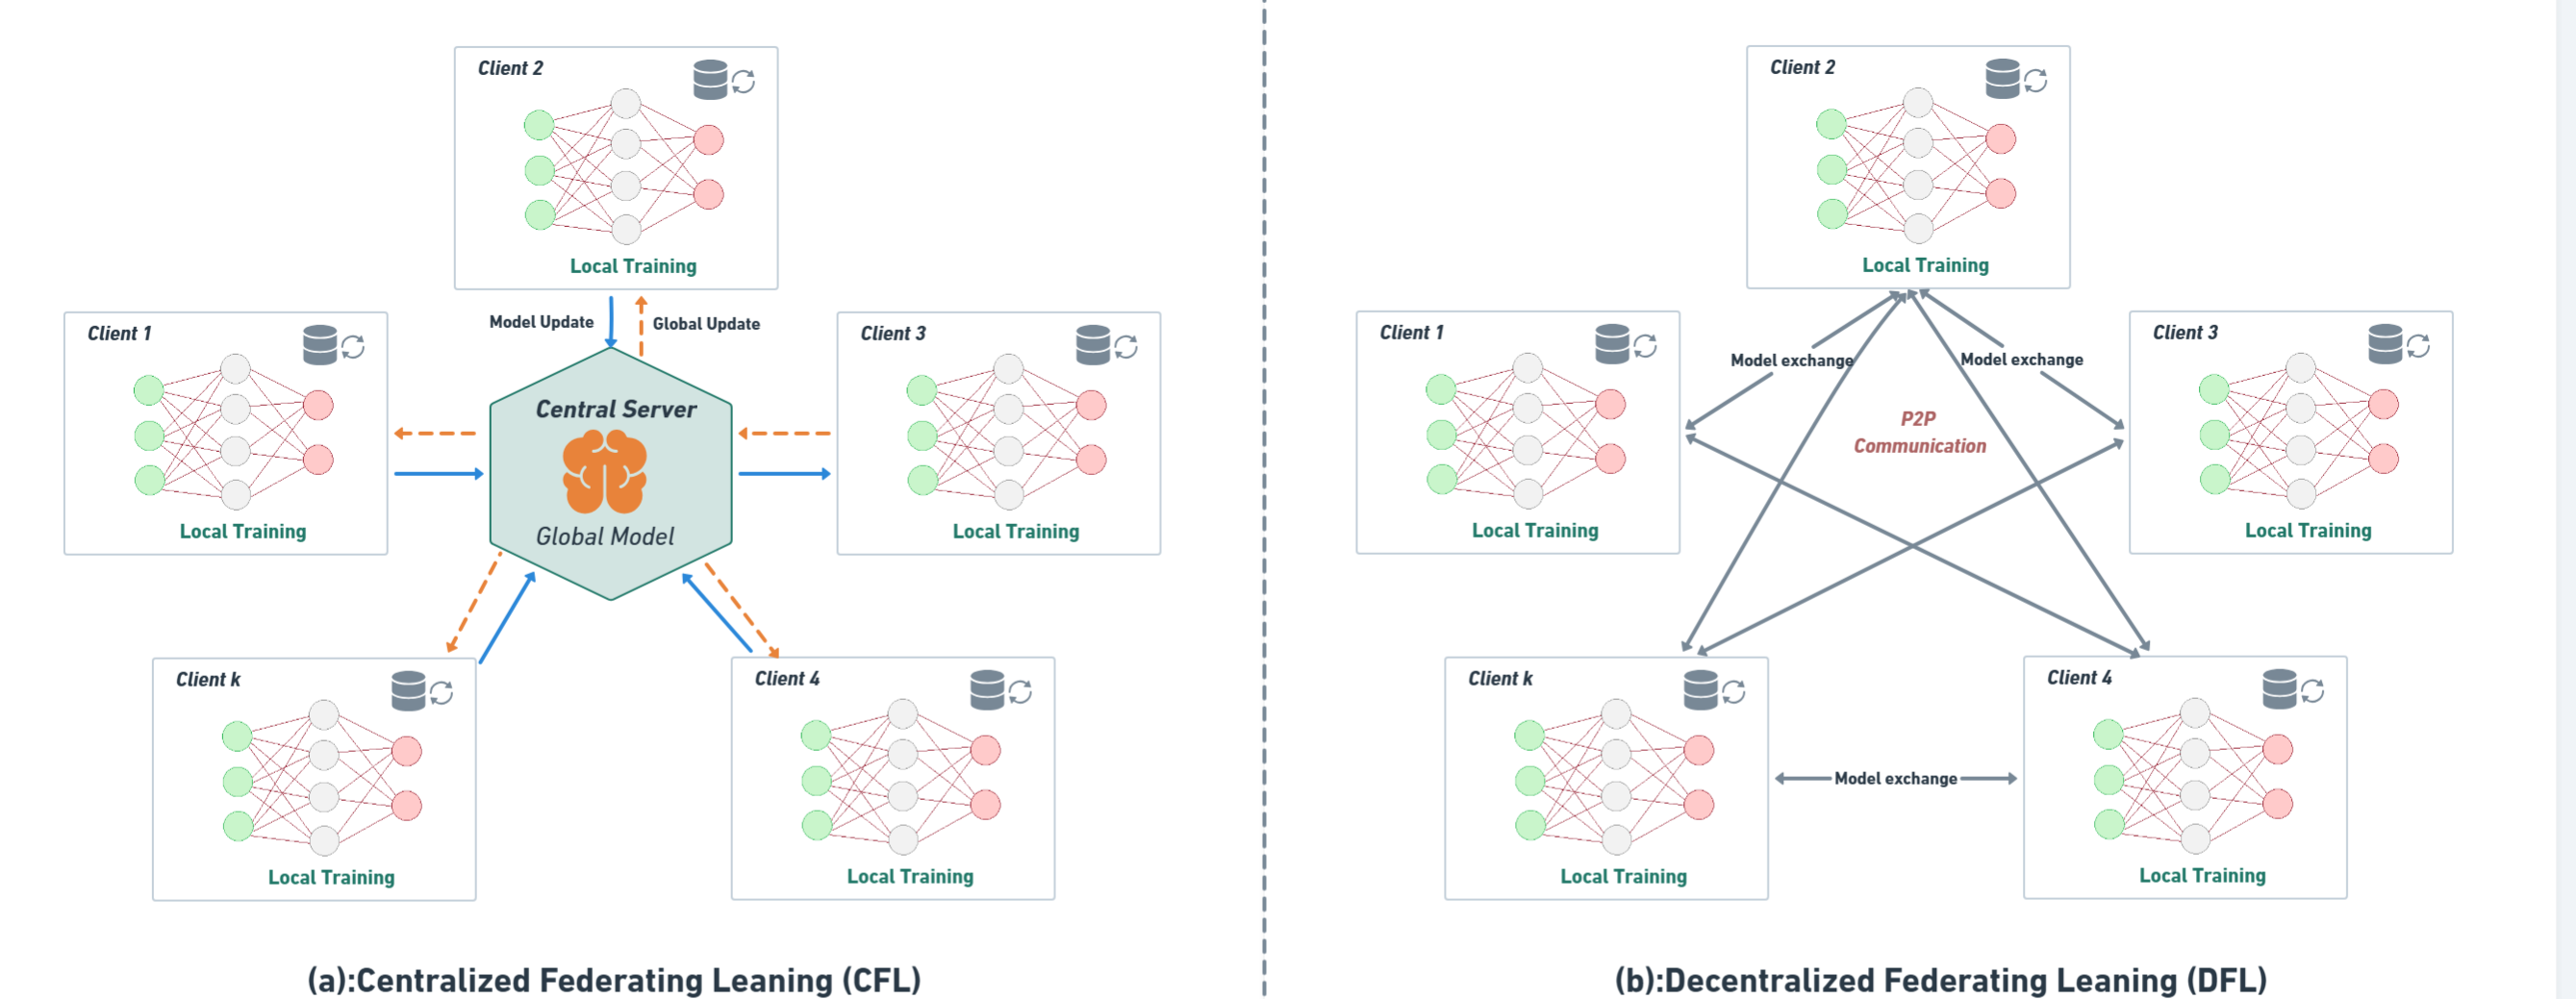
\includegraphics[width=1\linewidth]{Figures/network_based.png}
    \caption{Network Based Architecture}
    \label{fig:enter-label}
\end{figure}

Centralized Federated Learning (CFL) is a machine learning approach where a central server manages the coordination of training among multiple distributed clients. Each client trains a local model on its private data and periodically sends updates to the server. The server aggregates these updates to form a global model and redistributes it back to the clients. This setup allows data to remain local while still benefiting from collaborative learning across devices (Kairouz et al., 2021).

Decentralized Federated Learning (DFL) is a variation of federated learning that removes the need for a central server. Instead, clients communicate directly with each other in a peer-to-peer network to share model updates. Over time, these interactions lead to the development of a shared global model. DFL is particularly useful in environments where central coordination is not feasible or desired (Lalitha et al., 2019).




\section{Challenges and Solutions in Federated Learning}
\subsection{Privacy and Security Challenges}

Federated Learning (FL) faces significant challenges in maintaining data privacy and security during the collaborative training process. Since data remains on local devices, privacy-preserving techniques  such as encryption and differential privacy  are employed to prevent unauthorized access and ensure only aggregated model updates are shared [2].

Another major concern is the potential for malicious participants to inject biased or harmful updates into the training process. To mitigate this, secure aggregation protocols are implemented to verify the integrity and authenticity of model updates, ensuring the robustness of the final model.

 
% \subsubsection{Differential Privacy Techniques:}
% Differential privacy is a technique used to safeguard individual data privacy while permitting statistical analysis. In FL, differential privacy can be applied to add noise to the model updates before aggregation, avoiding the extraction of individual-level info.
% This practice helps to protect against membership inference attacks and statistical inference attacks on individual data [2].

\subsection{Communication and Resource Constraints}

Communication efficiency is crucial in FL, particularly when dealing with large-scale datasets or resource-constrained devices. To reduce communication overhead, techniques like model compression, quantization, and selective update transmission can be employed. These techniques reduce the amount of data transmitted between the local devices and the central server, which ultimately improves communication efficiency [2].
% \subsubsection{Bandwidth and Latency Constraints:}
% Bandwidth and latency constraints pose significant challenges in FL, mainly in scenarios with limited network resources. FL frameworks employ techniques such as gradient compression, adaptive communication scheduling, and bandwidth-efficient protocols to alleviate these constraints. These techniques aim to lessen the amount of data transmitted and optimize the communication schedule, reducing the impact of bandwidth and latency limitations.
% Adaptive Communication and Model Compression Techniques:
% Adaptive communication techniques automatically regulate the communication frequency or data exchanged based on the relevance of the local data. This allows more efficient utilization of network resources. Moreover, model compression techniques, such as knowledge distillation and pruning, can reduce the size of the model, supporting faster and more effective communication between the local devices and the central server [2].

\subsection{Heterogeneity and Data Distribution}
Data and Model Heterogeneity Handling Strategies:
FL frameworks need to deal with heterogeneity in terms of data types, formats, and model architectures among various participating devices. Techniques such as transfer learning meta-learning, and model aggregation with model selection can be used to handle heterogeneity. These approaches permit the central server to adjust and combine models trained on different types of data or models with varying architectures [2].
Federated Transfer Learning and Meta-Learning Approaches:
Federated Transfer Learning facilitates the transfer of knowledge from a pre-trained global model to local models, which helps increase learning productivity and performance [2].

% \subsection{Real-World Applications }
% While Federated Learning (FL) has been extensively explored in fields such as healthcare and finance, its application in environmental monitoring, particularly in water quality assessment, remains an emerging area of research. Recent studies have begun investigating its potential to enable privacy-preserving, real-time analysis of sensor data while addressing key challenges such as data heterogeneity and communication constraints. Existing projects leverage FL to enhance data privacy, computational efficiency, and scalability, particularly in real-time anomaly detection for water systems.
% One notable study introduces the MCN-LSTM (Multivariate Convolutional Neural Network with Long Short-Term Memory) approach for anomaly detection in water quality monitoring. This method integrates deep learning techniques to process and analyze large volumes of time-series data collected from IoT-enabled sensors. Unlike traditional centralized machine learning models, which require transferring raw environmental data to a central server, FL allows models to be trained locally on sensor nodes before aggregating updates in a decentralized manner, thereby improving data security and reducing bandwidth consumption.
% Several projects have explored FL for water quality prediction. For example, Wu et al. (2022) applied FL with LSTMs to monitor river water quality, achieving an RMSE of 0.12 pH units. Similarly, Zhang et al. (2023) used federated CNNs for detecting algal blooms from satellite imagery, demonstrating FL’s capability to process spatially distributed data while preserving data locality. Additionally, FL-based pollution tracking has been enhanced using anomaly detection methods such as Isolation Forest, which processes real-time data streams from distributed air and water sensors to identify sudden pollution spikes.
% Despite these advancements, FL-based approaches for water quality monitoring still 
% face significant technical barriers. Data heterogeneity remains a major challenge due to seasonal variations and the diversity of sensor types (e.g., pH probes vs. turbidity sensors), which can affect the consistency of model updates across decentralized nodes. Moreover, regulatory constraints, such as GDPR compliance, complicate cross-border data sharing in international water systems. These challenges highlight the need for more adaptive FL frameworks capable of operating across diverse environments while ensuring robust privacy, security, and computational efficiency.[3]

\newpage

\section*{Conclusion}


This chapter reviewed the current advancements in Federated Learning (FL), tracing its development from foundational concepts to recent innovations addressing scale and diversity. It covered various FL types based on data and network structures, showcasing FL's adaptability. While FL offers significant advantages, especially in privacy, it still faces challenges like security, communication overhead, and data heterogeneity, which are active research areas. The chapter also noted FL's emerging application in environmental monitoring, such as water quality, underscoring FL's growing importance for private, distributed data analysis.


























 % Assuming you might have this
\chapter{Background and System Methodology}
\label{chap:Chapter 3 title}
\section*{Introduction}
This chapter outlines the design and theoretical foundation of the proposed Water Quality Monitoring System using Federated Learning (FL). The methodology is built around a multi-layered system architecture comprising: the edge layer (data collection by water quality robots), the intermediate layer (LoRa gateway for data transmission, preprocessing, local model training), and the cloud layer (FL server for model aggregation, application server for system configuration). The chapter also details the data processing workflow, explaining how raw sensor data is collected, cleaned, stored, and utilized for federated learning, emphasizing privacy-preservation, scalability, and efficiency.


\newpage
\section{Background }
\subsection{Federated learning}

Federated Learning (FL) is revolutionizing machine learning by enabling decentralized modeling while preserving data privacy. Unlike traditional approaches that aggregate raw data into centralized servers, FL distributes a pre-trained global model to edge devices  such as smartphones, IoT sensors, and even low-cost hardware like Raspberry Pis  which then perform local training using their private data. This decentralized paradigm not only addresses privacy and regulatory concerns (e.g., GDPR compliance) but also reduces communication overhead, making it well-suited for dynamic and resource-constrained environments.


\subsection{Types of Federated Learning}
\subsubsection{Based on Data Distribution}

\textbf{Horizontal Federated Learning (HFL)}
\begin{figure}[H]
    \centering
    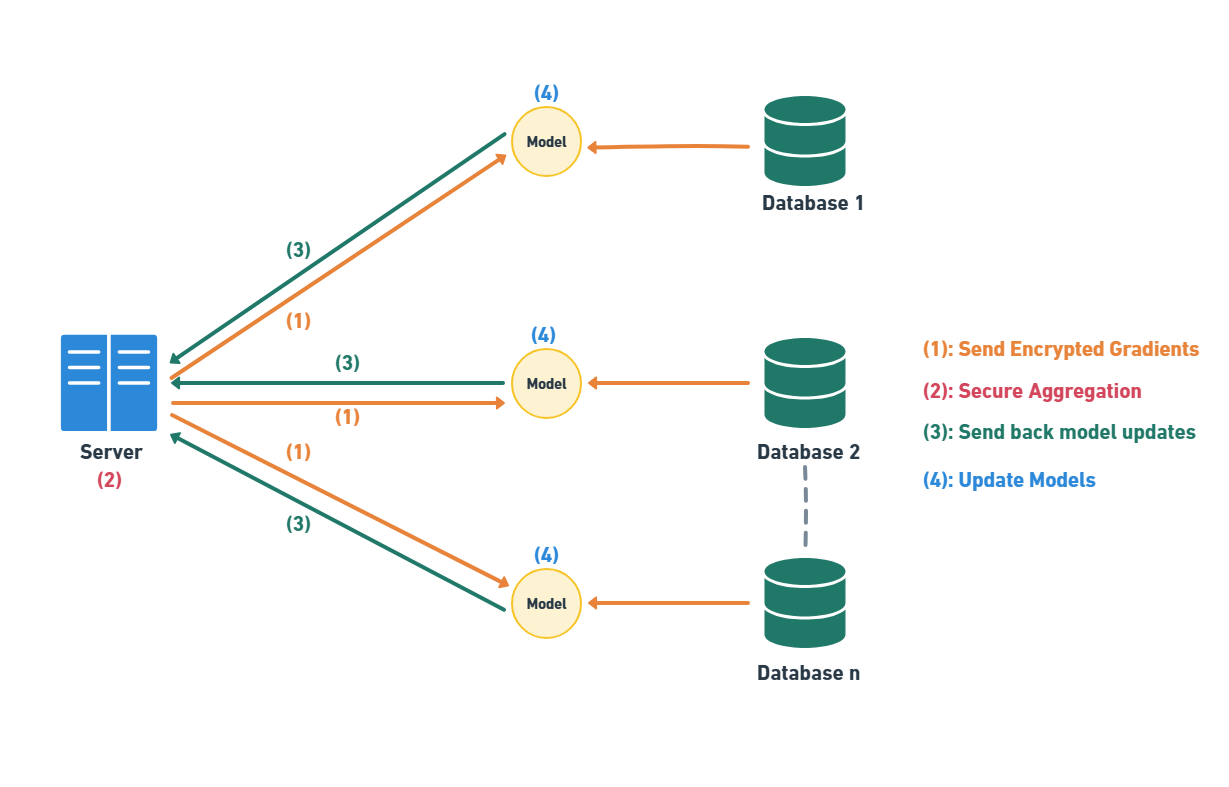
\includegraphics[width=0.75\linewidth]{Figures/diagram 1 (2).png}
    \caption{Horizontal Federated Learning}
    \label{fig:enter-label}
\end{figure}

Horizontal Federated Learning (HFL) is a decentralized machine learning approach in which multiple participants collaboratively train a shared global model without exchanging raw data. Each participant holds datasets with the same feature space, such as hospitals collecting identical health metrics, but with different data samples, ensuring both data privacy and compliance with protection regulations.

\textbf{Vertical Federated Learning (VFL)}
\begin{figure}[H]
    \centering
    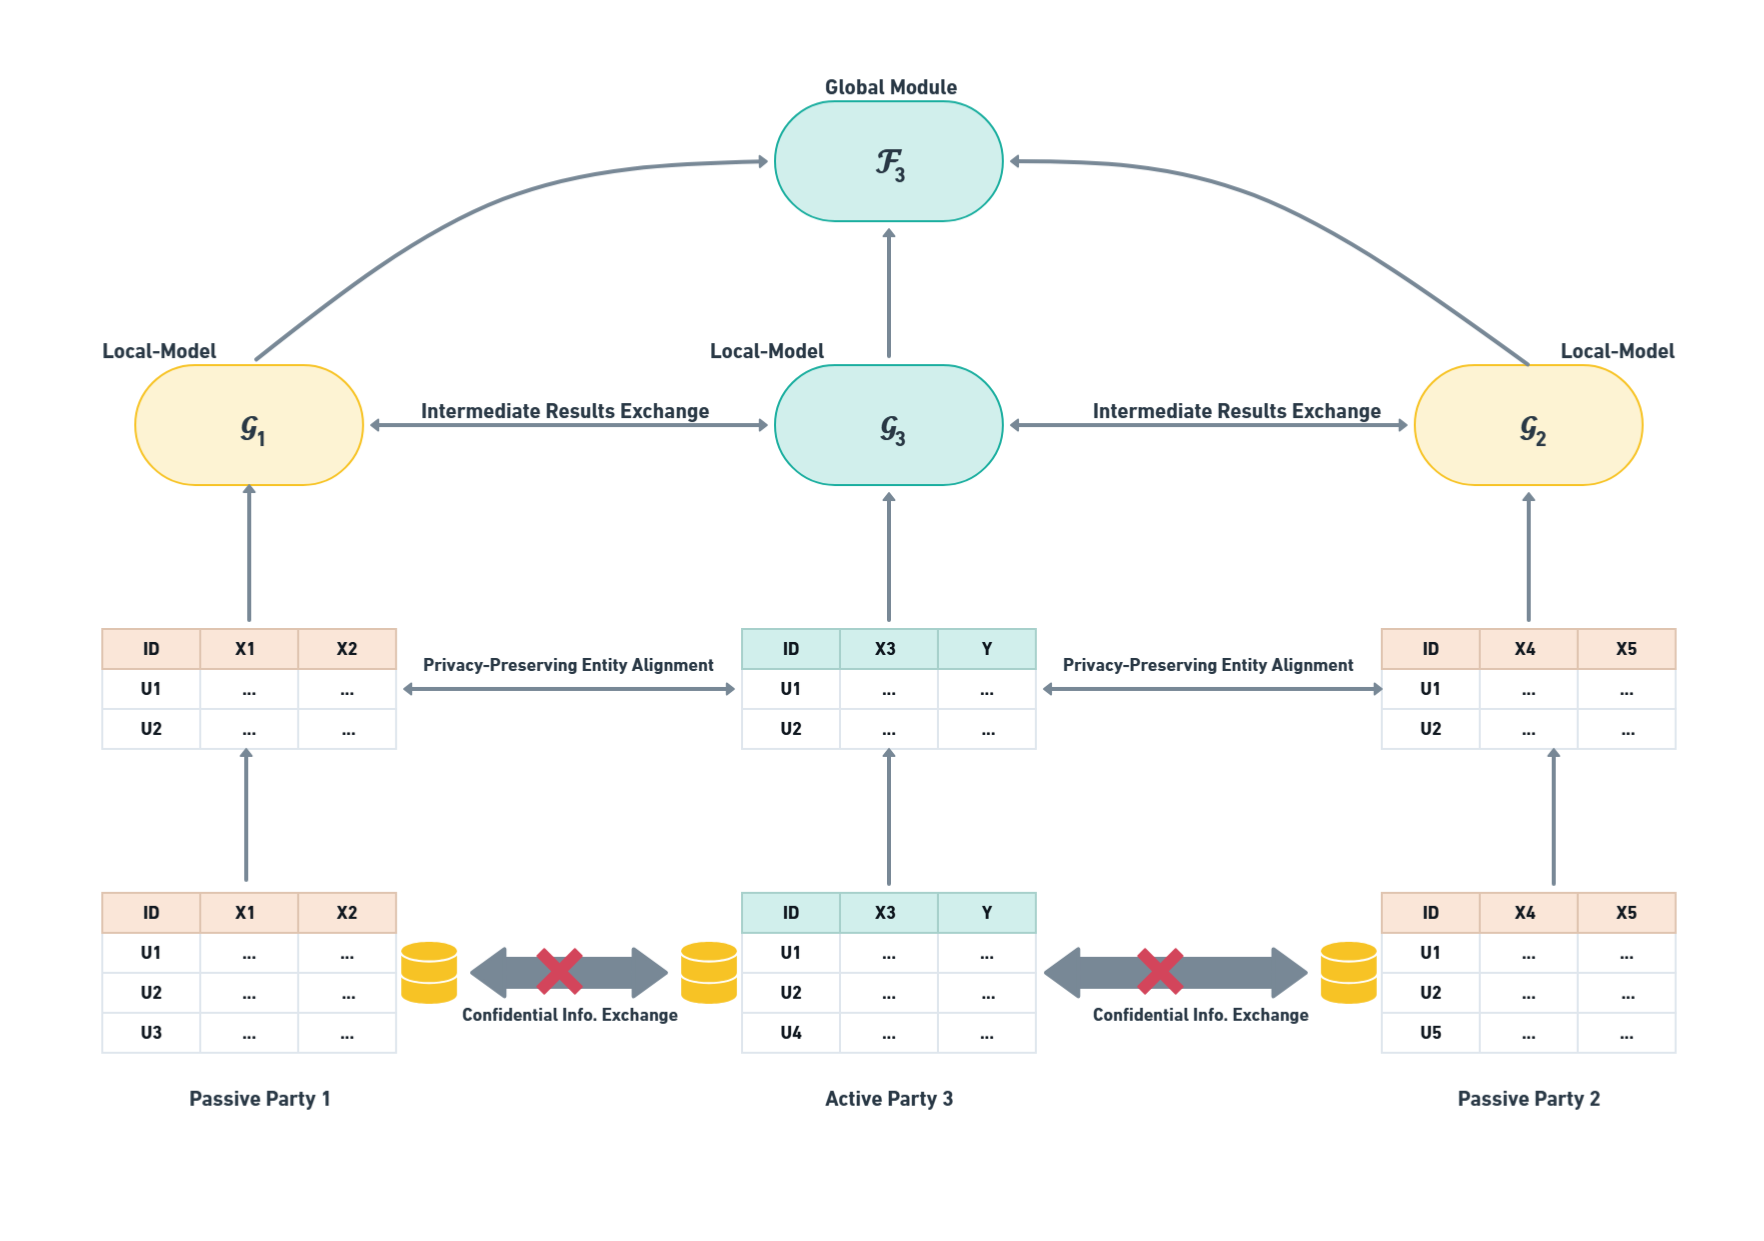
\includegraphics[width=0.75\linewidth]{Figures/VFL.png}
    \caption{Vertical Federated Learning}
    \label{fig:enter-label}
\end{figure}

Vertical Federated Learning (VFL) is tailored for scenarios where different organizations possess complementary features about the same individuals. For example, a bank can have access to a customer’s financial records, while a retailer holds their purchase history. By collaborating, these entities can train a more comprehensive model without revealing their raw data. In VFL, the feature space is partitioned, which means that each participant has a distinct subset of features for the same set of users,

\subsubsection{Based On Network Structure}

\begin{figure}[H]
    \centering
    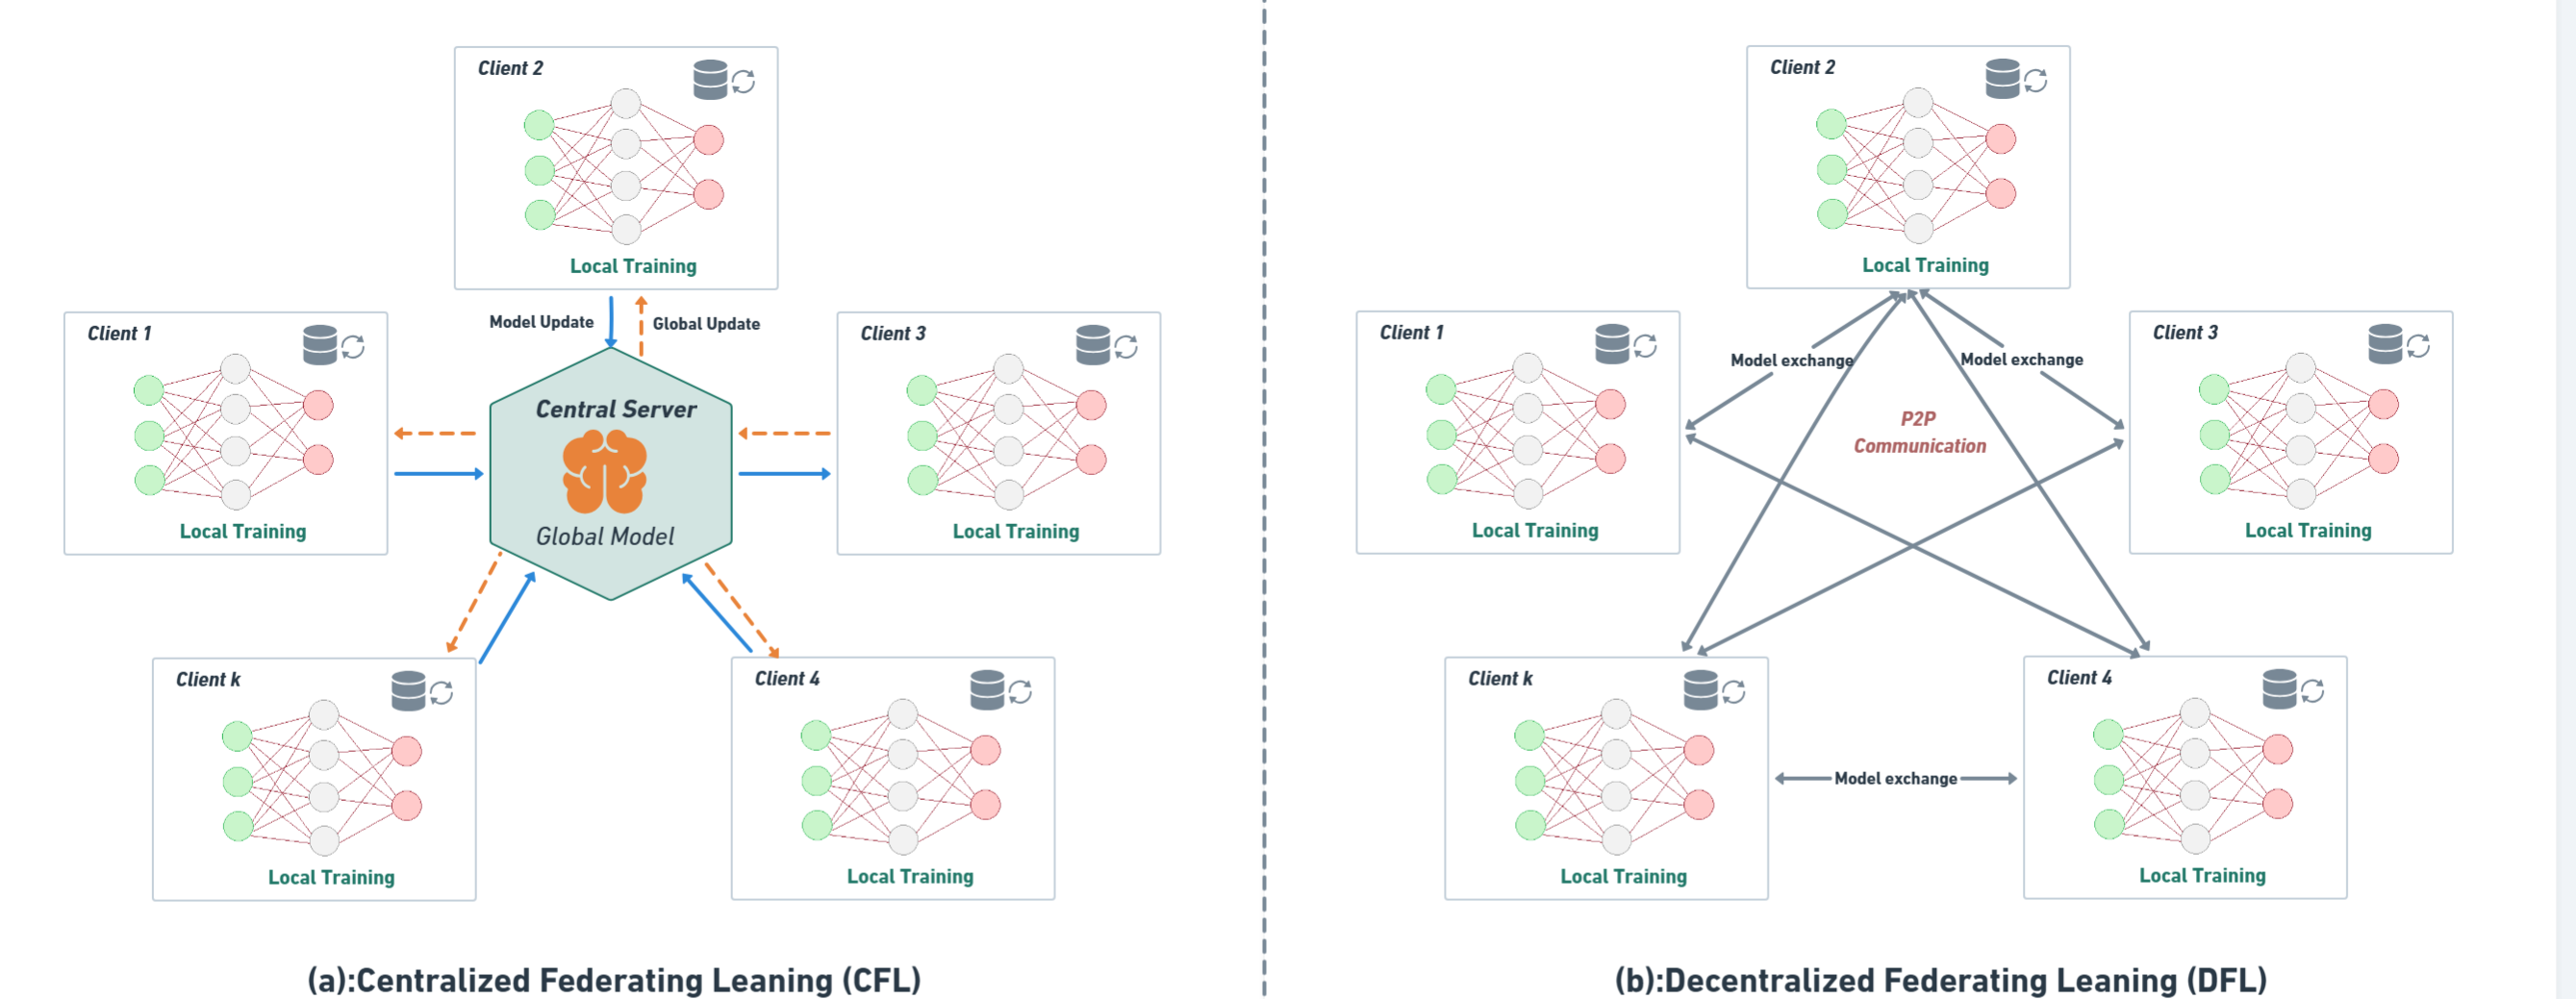
\includegraphics[width=1\linewidth]{Figures/network_based.png}
    \caption{Network Based Architecture}
    \label{fig:enter-label}
\end{figure}

Centralized Federated Learning (CFL) is a machine learning approach where a central server manages the coordination of training among multiple distributed clients. Each client trains a local model on its private data and periodically sends updates to the server. The server aggregates these updates to form a global model and redistributes it back to the clients. This setup allows data to remain local while still benefiting from collaborative learning across devices (Kairouz et al., 2021).

Decentralized Federated Learning (DFL) is a variation of federated learning that removes the need for a central server. Instead, clients communicate directly with each other in a peer-to-peer network to share model updates. Over time, these interactions lead to the development of a shared global model. DFL is particularly useful in environments where central coordination is not feasible or desired (Lalitha et al., 2019).

\subsection{Challenges and Solutions in Federated Learning}
\subsubsection{Privacy and Security Challenges}

Federated Learning (FL) faces significant challenges in maintaining data privacy and security during the collaborative training process. Since data remains on local devices, privacy-preserving techniques  such as encryption and differential privacy  are employed to prevent unauthorized access and ensure only aggregated model updates are shared [2].

Another major concern is the potential for malicious participants to inject biased or harmful updates into the training process. To mitigate this, secure aggregation protocols are implemented to verify the integrity and authenticity of model updates, ensuring the robustness of the final model.


\subsubsection{Communication and Resource Constraints}

Communication efficiency is crucial in FL, particularly when dealing with large-scale datasets or resource-constrained devices. To reduce communication overhead, techniques like model compression, quantization, and selective update transmission can be employed. These techniques reduce the amount of data transmitted between the local devices and the central server, which ultimately improves communication efficiency [2].


\subsubsection{Heterogeneity and Data Distribution}
Data and Model Heterogeneity Handling Strategies:
FL frameworks need to deal with heterogeneity in terms of data types, formats, and model architectures among various participating devices. Techniques such as transfer learning meta-learning, and model aggregation with model selection can be used to handle heterogeneity. These approaches permit the central server to adjust and combine models trained on different types of data or models with varying architectures [2].
Federated Transfer Learning and Meta-Learning Approaches:
Federated Transfer Learning facilitates the transfer of knowledge from a pre-trained global model to local models, which helps increase learning productivity and performance [2].



\section{System Design and Architecture}
\label{sec:system_design_and_architecture}

\subsection{General System Overview}
\label{ssec:general_system_overview}

The proposed Water Quality Monitoring System is a multilayered system that combines Internet of Things (IoT), Edge Computing, and Federated Learning (FL) technologies to provide a scalable and privacy-preserving solution for real-time water quality monitoring. As illustrated in Figure \ref{fig:system_architecture_high_level_overview}, the system has three main layers: the Edge Layer, the Intermediate Layer, and the Cloud Layer, each with respective roles that collectively facilitate intelligent data acquisition, localized processing, secure communication, and global model training.

\begin{figure}[H]
    \centering
    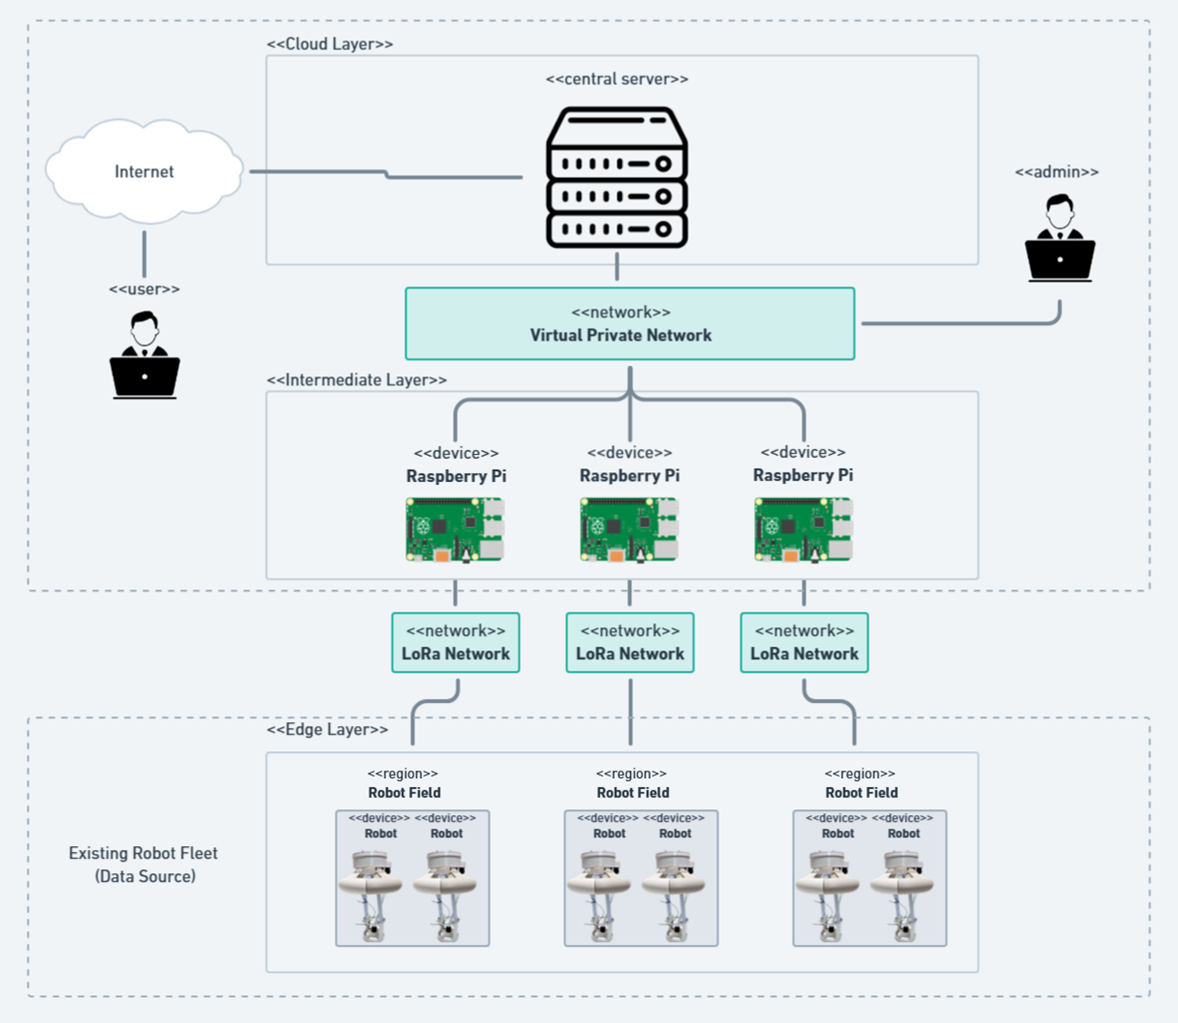
\includegraphics[width=0.75\linewidth]{Figures/system_architecture.png}
    \caption{General System Overview Diagram} % Updated Caption
    \label{fig:system_architecture_high_level_overview} % Updated Label
\end{figure}

The Edge Layer of the system consists of Water Quality Robots deployed in aquatic environments to enable distributed monitoring. The robots collect key water quality parameters and have low-power communication capabilities that allow them to transmit data wirelessly to the Intermediate Layer.

The Intermediate Layer, centered on Raspberry Pi units, functions as a bridge between sensor-equipped robots and the cloud infrastructure. It is responsible for aggregating data from multiple edge devices and performing a comprehensive preprocessing pipeline, including threshold-based filtering, basic machine learning-based anomaly detection, dynamic data cleaning. Furthermore, it initiates a federated learning process, training local machine learning models on the sanitized data and transmitting only encrypted model weight updates to the cloud.

Finally, the Cloud Layer serves as the central command and aggregation point. It comprises a Federated Learning server dedicated to orchestrating the global model aggregation process from updates received from various Intermediate Layer gateways. Alongside this, an Application Server manages overall system configurations, provides monitoring dashboards, and facilitates user interaction with the system.


\subsection{Detailed System Architecture and Component Breakdown} % Updated Subsection Title
\label{ssec:detailed_architecture_components}

The architecture depicted in Figure \ref{fig:global_architecture_detailed_components} illustrates a comprehensive and secure system designed for water quality monitoring, leveraging intelligent data processing through edge computing and federated learning. This diagram highlights the data flow and key interactions between components across the distinct system layers.

\begin{figure}[H]
    \centering
    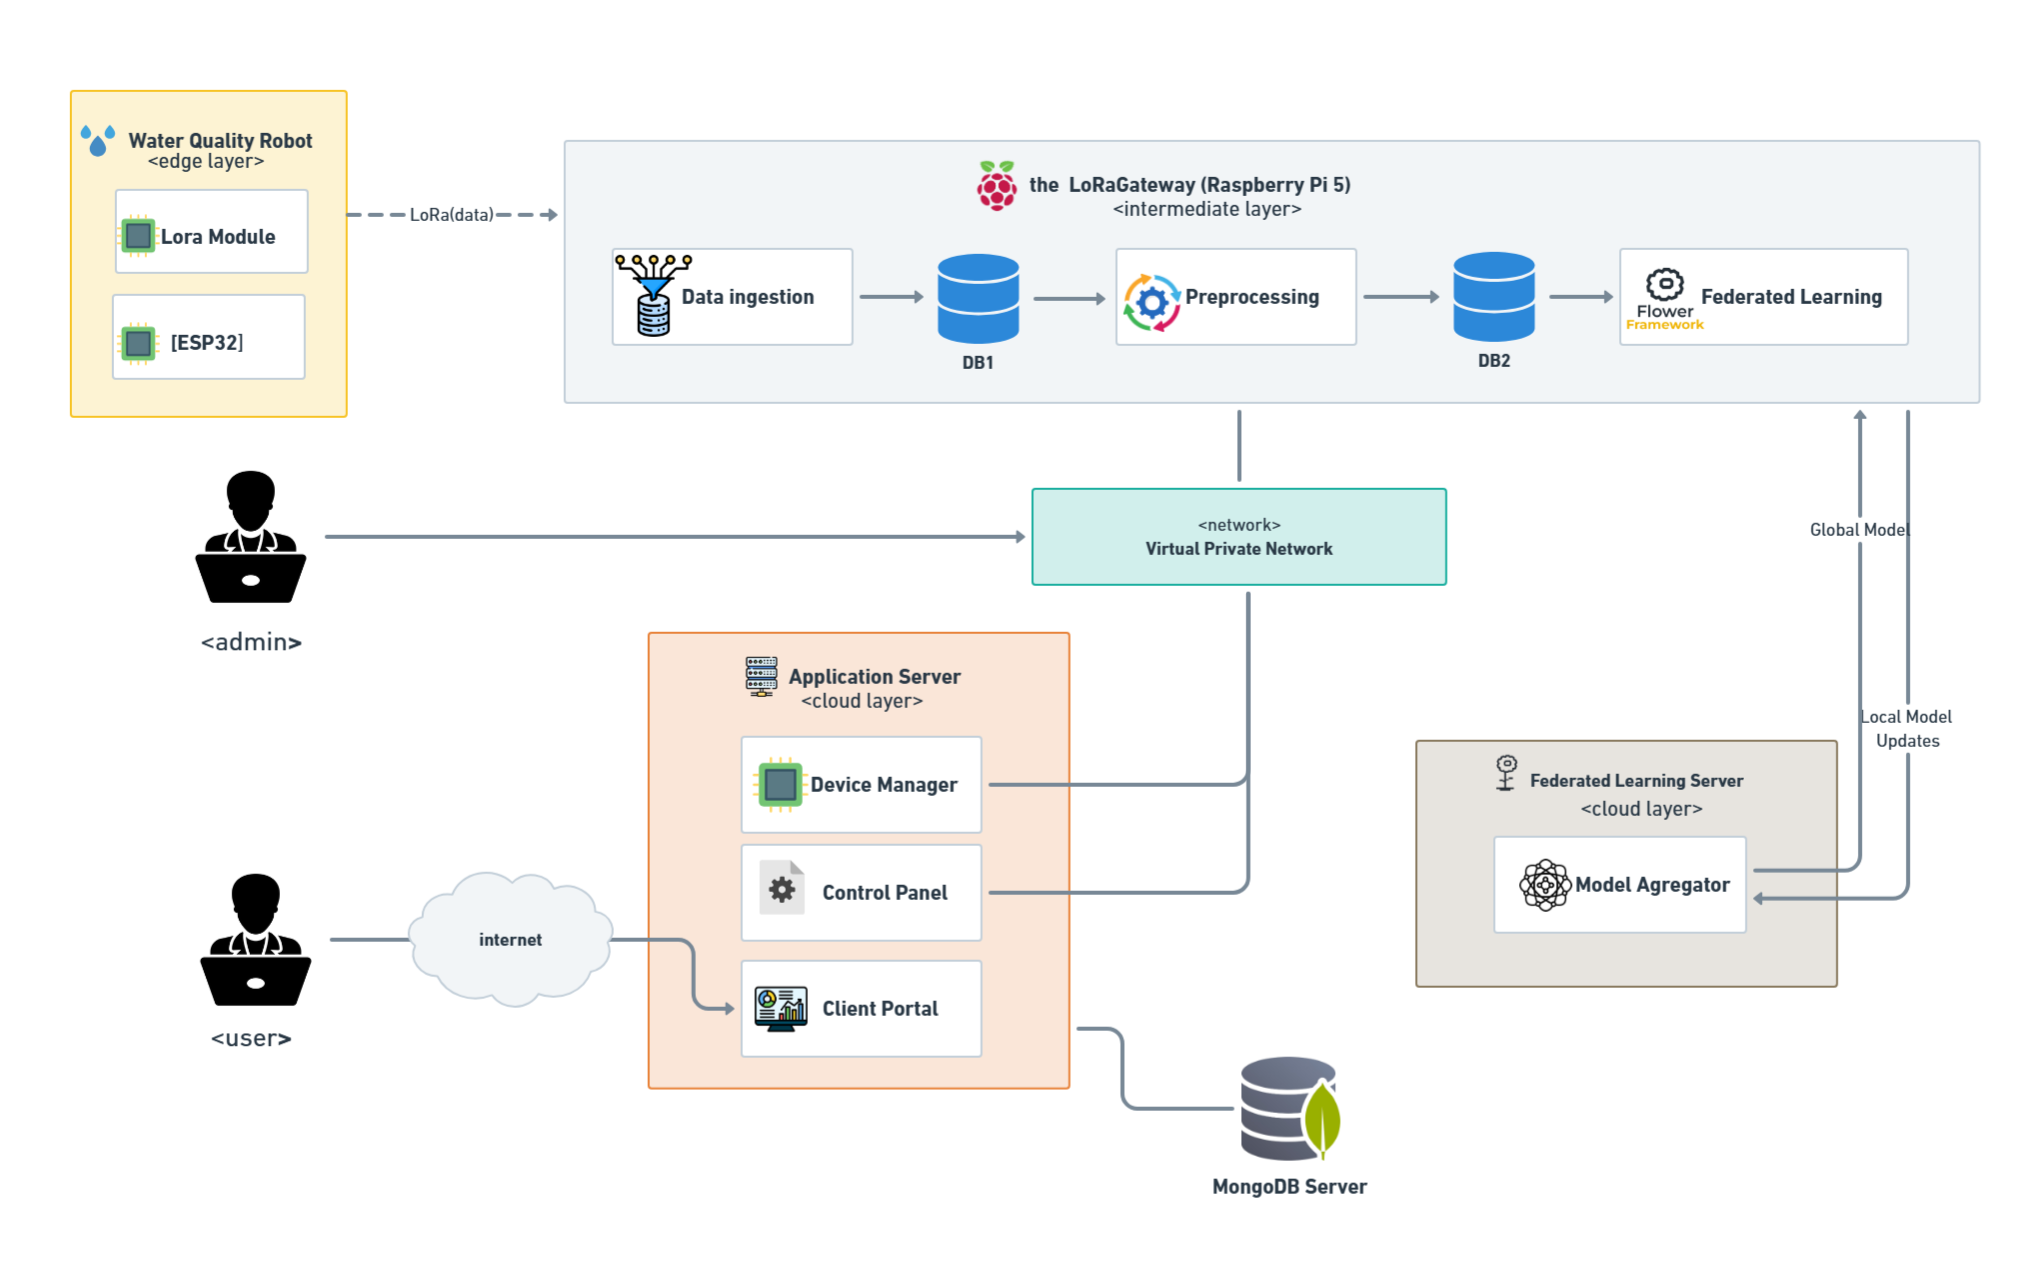
\includegraphics[width=0.75\linewidth]{Figures/GArchi1.png}
    \caption{Detailed Component Architecture Diagram}
    \label{fig:enter-label}
\end{figure}



Upon complete implementation, the edge layer will use Water Quality Robots as the primary data acquisition units. The design of these robots is based on the low-cost open-source smart buoy developed within the SmartWater project in Brussels, as detailed by Quevy et al. (2023). These autonomous robots will be equipped with a series of sensors to measure key water quality parameters, including pH, temperature, dissolved oxygen, conductivity, and potentially turbidity, consistent with the capabilities of the referenced buoy design. An ESP32 microcontroller will manage the onboard control and preliminary data processing, while a LoRa module will ensure long-range wireless communication. Sensor data, temporarily stored and formatted by the ESP32, will be transmitted via the LoRa protocol to a Raspberry Pi 5-based LoRa Gateway, a central component of the Intermediate layer.

Once the Raspberry Pi 5 in the intermediate layer receives raw data from these edge robots, it initiates a data processing pipeline. This begins with Data Ingestion, where incoming packets are decoded, transformed into a structured format, and stored temporarily in a local database (DB1). Following this, the Preprocessing phase applies filtering rules and machine learning models to detect anomalies and clean the data, with the resulting refined data stored in DB2, ready for training and analytics.

The core strength of this system lies in its integration of federated learning. The Raspberry Pi utilizes its private, preprocessed data from DB2 to train a local machine learning model using the Flower Federated Learning framework. Critically, only encrypted model updates are transmitted to the Federated Learning Server, which resides in the cloud layer and hosts a Model Aggregator. This server then aggregates updates from multiple participating gateways to build an improved global model, which is subsequently distributed back to the gateways. This iterative process enhances model accuracy while ensuring data privacy and decentralization.

The Raspberry Pi communicates with the Application Server in the cloud layer via APIs to receive configuration parameters and exchange operational data. The administrator can access the Application Server via a secure VPN to interact with its key components. The Control Panel provides full administrative control over the machine learning pipeline, including hyperparameter tuning, selection of anomaly detection methods, and regulation of the federated learning server. It also offers detailed statistics on system performance, anomaly reports, warnings, and notifications. The Control Panel allows the administrator to monitor and manage the operational status of all connected devices. In contrast, regular users can access only the Visualization Module, which provides a read-only interface for viewing historical and predicted WQI data. All relevant metrics and logs are persistently stored in a MongoDB server within the cloud infrastructure.

\subsubsection{Edge Layer}
\label{sssec:edge_layer_detail} % Now a subsubsection
The Edge Layer is envisioned as the primary data acquisition front-end of the Water Quality Monitoring System, responsible for direct in-situ environmental measurements. In the target deployment, this layer would consist of autonomous Water Quality Robots. The design specifications for these robots are based on the open-source "Smart Buoy" detailed by Quevy et al. in "Open Sensing System for Long Term, Low Cost Water Quality Monitoring" [*********** Reference Number for the Paper**************], selected for its proven capabilities in environmental sensing and LoRa communication.

These conceptual Water Quality Robots would incorporate an ESP32 microcontroller, a standard suite of sensors for parameters such as pH, temperature, dissolved oxygen (DO), electric conductivity (EC), and turbidity, and an RFM95W LoRa module for data transmission, mirroring the hardware architecture of the referenced Smart Buoy.

For the current phase of this research and system development, the data input from the Edge Layer is simulated using historical water quality datasets , built around an ESP32 and an RFM9x LoRa module, is utilized to send formatted data packets representative of what an actual Water Quality Robot would generate. This approach allows for the development and testing of the Intermediate Layer gateway, the Cloud Layer functionalities, and the federated learning mechanisms without requiring immediate deployment of the full physical robot fleet.

The function of this Edge Layer is therefore to provide periodic water quality data, which is then transmitted via LoRa to an Intermediate Layer gateway. This allows the project to focus on the data processing, communication protocols, and the federated learning architecture using realistic data inputs.
%TODO:
\subsubsection{Intermediate Layer}
\label{sssec:intermediate_layer_detail} % Now a subsubsection
The Intermediate Layer serves as a crucial local processing and learning hub, built around a gateway. This gateway is responsible for data ingestion, collecting raw sensor data from distributed Edge Layer robots.

\textbf{Gateway Hardware}

The gateway's hardware is centered around a \textbf{Raspberry Pi 5 with 8GB of RAM}, providing ample processing power for local data tasks and machine learning model training. For communication with the edge devices, it is equipped with an \textbf{Adafruit RFM95W LoRa Radio Transceiver Breakout}. This module facilitates the reception of data transmissions directly from the edge layer robots operating on the LoRa protocol. For local data storage, including raw sensor readings and processed datasets, the gateway utilizes a \textbf{64GB Class 10 microSD card}. The entire gateway assembly is powered by a 5V 5A power supply unit.


\textbf{Outlier Detection}

Collected data is first analyzed for anomalies. Using rule-based checks or lightweight machine learning, the gateway identifies outliers to prevent corrupted inputs from impacting the learning process. Anomaly metadata is retained and reported to the Application Server for transparency and long-term system oversight. The Application Server allows remote tuning of thresholds, detection methods, and update frequencies to adapt to changing environmental conditions or operational needs.

\textbf{Data Cleaning and Imputation}

Before imputation, the gateway trains local cleaning models to estimate missing values based on historical patterns. These models are updated periodically, and their performance is monitored. Accuracy metrics are reported to the Application Server. Once trained, these models are used in real time to impute missing or flagged data, ensuring the quality and consistency of training data. The Device Manager enables centralized control over model types, training intervals, and fallback strategies.

\textbf{Federated Learning Model Development and Training}

\label{par:fl_model_dev_train} % Label for paragraph if needed
The development and training of the Water Quality Index (WQI) predictive model in the gateway follow a structured two-stage approach.
\begin{enumerate}
    \item \textbf{Centralized Model Optimization:}
    
        Prior to federated deployment, an initial phase of centralized machine learning experimentation is conducted. This phase utilizes historical water quality datasets to:
        \begin{itemize}
            \item Perform feature engineering to derive a rich set of potential predictors from the base sensor readings and temporal information.
            \item Conduct iterative feature reduction and selection, evaluating feature importance to identify an optimal, parsimonious feature set.
            \item Explore various Recurrent Neural Network (RNN) architectures to determine a robust model structure suitable for time-series WQI prediction.
        \end{itemize}
        The primary outcome of this centralized stage is the selection of the more promising model architectures and their corresponding optimized feature sets.
    \item \textbf{Federated Learning Implementation:}
    
        With a well-defined model architecture and feature set derived from the centralized optimization phase, the gateway then participates in the federated learning process. Using the locally preprocessed and cleaned data, the gateway trains this selected local model as part of the Flower federated learning framework (as depicted in Figure \ref{fig:global_architecture_detailed_components}). It engages in regular training rounds orchestrated by the Federated Learning Server, contributing only its model updates (weights and gradients) rather than raw data. Ensuring data privacy, minimizes network load, and enables the collaborative building of a global WQI prediction model through decentralized intelligence.
\end{enumerate}

\textbf{Model Exploitation}

After completing the federated learning training and receiving an updated global model, the gateway waits for a signal from the Application Server before utilizing the locally refined model to make predictions on new incoming data. This ensures that predictions are based on the most current model version, and the gateway processes data locally without immediate server interaction for this inference step. Predictions are then transmitted to the Application Server for visualization and potential alert generation.


\textbf{Operational Workflow}

% The operational workflow at this gateway begins with data ingestion. Raw sensor data, received via LoRa from the distributed robots, is stored locally in its raw form (DB1 in Figure \ref{fig:global_architecture_detailed_components}) before undergoing further processing. A key characteristic of this architecture is that this layer does not transmit raw data to the cloud. Instead, it processes the data locally, shares only notifications and statistics with the Application Server, and actively participates in federated learning. Critical aspects of this layer's processing pipeline, such as outlier detection strategies and the training of cleaning models, are dynamically configurable via the Application Server .
The operational workflow starts with data collection from Sensors and Data Acquisition. For model training, Historical Data undergoes Outlier Detection and Data Cleaning before being used in a Federated Learning cycle; this involves local model training and server-based aggregation to create an improved global model. Separately, for prediction, recent Last Data Samples are also cleaned and fed into The best saved model to Predicting future values, which are then reported to the Server.
\begin{figure}[H]
    \centering
    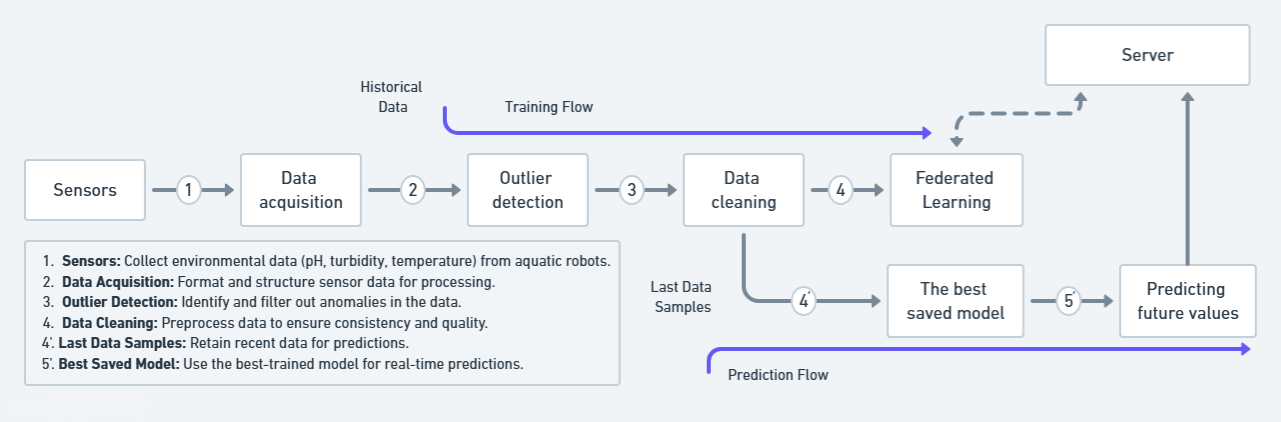
\includegraphics[width=1\linewidth]{Figures/Data Workflow.png}
    \caption{Data Processing Flow Diagram}
    \label{fig:enter-label}
\end{figure}

\subsubsection{Cloud Layer}
\label{sssec:cloud_layer_detail} % Now a subsubsection

\textbf{Federated Learning Server}

he Federated Learning Server coordinates the aggregation of locally trained model updates from gateways within the distributed system. Instead of centralizing data, each gateway trains a model on its local data and sends only weight updates to the server. These updates are combined using a federated averaging strategy to create a new global model, which is then redistributed to all gateways for the next training round. This iterative process enables continuous learning while preserving data privacy.

\textbf{Application Server}

The Application Server operates as a core software component hosted on the central AWS EC2 instance, alongside the Federated Learning Server and MongoDB. The cloud infrastructure, including these services, is secured using an OpenVPN server also running on the EC2 instance, establishing encrypted tunnels for communication with Intermediate Layer gateways.
It serves as the centralized control point for the overall Water Quality Monitoring System, bridging user interfaces with the gateways and the Federated Learning Server. As depicted in Figure \ref{fig:global_architecture_detailed_components}, it comprises several distinct modules:

\textbf{1. Client Portal }
The Client Application is a user-facing web platform that provides accessible water quality information and monitoring features to the public. It offers interactive tools such as regional water quality maps, real-time sensor data, and historical trends. Users can explore key features like environmental parameters and predictive analytics, and register to receive timely alerts on water quality changes in selected regions. The application focuses on delivering clear, actionable insights through an intuitive interface, supporting informed decision-making and community engagement.

\textbf{2. System Management Console (Control Panel):}
This Component provides secure administrator authentication and centralized control over system configurations and device management. Authorized administrators can onboard devices, adjust region-specific parameters  including anomaly detection thresholds and data cleaning models  and manage the scheduling of federated learning tasks such as model training and prediction. The module also delivers real-time monitoring and visualization of system notifications, anomaly occurrences, model performance metrics, and active alerts. All configuration and monitoring capabilities are accessible exclusively through a secured administrative interface.

\textbf{3. Device Management (Device Manager):}

% This component is central to managing interactions with the intermediate clients. It serves as the primary coordination point for dispatching operational commands to these distributed nodes, such as initiating federated model training cycles or triggering water quality prediction routines. To ensure these distributed tasks are performed reliably and at appropriate intervals. Furthermore, it is responsible for delivering client-specific configurations necessary for their operation and for processing the various outputs received from the devices, notably including operational alerts and crucial environmental data like water quality predictions.
This component directly manages and interacts with intermediate layer clients, primarily by delivering client-specific configurations to enable their designated tasks. It then serves as the central hub for dispatching operational commands like initiating model training or prediction routines based on system schedules, utilizing an internal scheduling mechanism for reliable execution. The Device Manager also processes outputs from these clients, handling operational alerts and ingesting their water quality predictions.

\newpage

\section*{Conclusion}
This chapter comprehensively outlined the methodological framework for the proposed Water Quality Monitoring System using Federated Learning. It detailed a robust multilayered architecture (edge, intermediate, cloud layers) with distinct, interconnected roles, from distributed data acquisition by autonomous robots to global model aggregation and system management. The critical functions of the intermediate LoRa gateway, encompassing data ingestion, preprocessing, local database management, and local model training, were elucidated, highlighting its role as a crucial hub for localized intelligence. Similarly, the responsibilities of the cloud layer, with its dedicated Federated Learning server for model aggregation and an Application Server for system configuration, monitoring, and user interaction, were thoroughly described. Furthermore, the chapter presented the data processing workflow, illustrating the systematic progression from raw sensor readings through cleaning and imputation to their effective utilization in the federated learning process for generating and refining predictive models. The strategic adoption of Federated Learning was central to this methodology, enabling a system that inherently ensures data privacy by keeping raw data localized, promotes scalability by distributing computational load, and enhances efficiency by minimizing communication overhead.

\pagebreak
\chapter{Implementation}
\label{chap:Chapter 4 title}


\section*{Introduction}
Following the methodological framework detailed in the preceding chapter, this chapter delves into the practical implementation of the Federated Learning system for Water Quality Monitoring. It provides a comprehensive account of the software components developed, the system integration strategies employed, and the specific technical choices made to bring the conceptual design to life.

The chapter begins by describing the simulation of real-time data collection, a crucial step for testing and validation in the absence of a fully deployed physical sensor network. It then elaborates on the intricacies of the data preprocessing pipeline executed on the edge devices, covering anomaly detection techniques, data cleaning, imputation models, and the notification system designed to report operational metrics.

Subsequently, the implementation of the core Federated Learning workflow is detailed, including client participation and server-side aggregation. A significant portion is dedicated to feature engineering for enhanced water quality prediction and the integration of these features into Recurrent Neural Network (RNN) models. Security, a paramount concern, is addressed through the implementation of mutual TLS (mTLS) and TLS for secure communication between system components. Finally, the chapter outlines the development of the backend infrastructure and the user-facing web interfaces both for client users and system administrators highlighting the technologies used and the functionalities provided.

\pagebreak



\section{Software Components and System Integration}

\subsection{Data Injection and Simulation}
To simulate real-time data collection from water quality monitoring robots, we relied on historical datasets containing time-series measurements of various parameters such as temperature, pH level, dissolved oxygen, turbidity, and conductivity. These datasets acted as stand-ins for actual sensor streams, allowing us to create a controlled and repeatable environment to test the local preprocessing and federated learning workflows deployed on each Raspberry Pi.

The simulation process was implemented via custom Python scripts that sequentially read data samples from CSV files and injected them into local SQLite databases hosted on each Raspberry Pi. The design aimed to mimic the behavior of real sensors pushing data in a streaming fashion, with control over the injection rate to simulate different sampling frequencies.

Each Raspberry Pi runs the injection script independently, creating a decentralized simulation environment. The data is written into a local SQLite table structured to reflect the schema expected by the preprocessing pipeline, including timestamps and all relevant water quality indicators. This modularity allowed us to test anomaly detection, cleaning, and training pipelines as if the data were being generated live.

\textbf{Pseudocode of the Simulation Process:}

\begin{algorithm}[H]
    \caption{Simulated Sensor Data Injection}
    \label{alg:sensor_injection}
    \SetAlgoLined
    \KwIn{
        Historical dataset $D$ (CSV), \\ \vspace{0.1cm}
        SQLite connection $db$, \\ \vspace{0.1cm}
        Injection interval $\Delta t$\vspace{0.1cm}
    }
    \KwOut{
        Time-series sensor data written into local SQLite database
    }
    
    \Begin{
        Initialize table schema in $db$\; \vspace{0.1cm}
        $rows \leftarrow$ read rows from $D$\; \vspace{0.1cm}
        
        \ForEach{$row \in rows$}{
            $timestamp, temperature, pH, oxygen, turbidity, conductivity \leftarrow row$\; \vspace{0.1cm}
            Insert $row$ into SQLite table\; \vspace{0.1cm}
            Sleep for $\Delta t$ seconds to simulate real-time input\; \vspace{0.1cm}
        }
    }
\end{algorithm}





\subsection{Preprocessing}
\subsubsection{Anomaly Detection}
This module aims to detect anomalous sensor readings in water quality data using three distinct methods, selected based on configuration parameters. The goal is to flag outlier values that may indicate faulty sensors, environmental issues, or data corruption.

The process begins with parsing and formatting the time field, ensuring temporal consistency. The algorithm then identifies the most frequently occurring date in the dataset, referred to as the batch\_day, which is used later for reporting and notification purposes.

Depending on the specified detection method (rule\_based, IQR, or decision\_tree), the algorithm applies one of the following techniques:

\textbf{Rule-based detection }involves checking whether each reading of pH, conductivity, temperature, or dissolved\_oxygen falls within predefined minimum and maximum acceptable.
\newline
\textbf{Interquartile Range (IQR)} method calculates the first (Q1) and third (Q3) quartiles for each numeric column. It then determines the IQR (Q3 - Q1) and flags values that fall outside the range [Q1 - 1.5×IQR, Q3 + 1.5×IQR], which are considered statistical outliers.

\textbf{Decision Tree method} trains a model for each target variable using the remaining variables as predictors. Any significant deviation between the actual and predicted values indicates a potential anomaly, which is flagged accordingly.

At the end of the process, the algorithm returns an updated DataFrame with boolean flags and a summary dictionary containing counts of anomalies per feature.

\begin{algorithm}[H]
    \caption{Anomaly Detection in Sensor Data}
    \label{alg:anomaly_detection}
    \KwIn{
        Raw sensor data DataFrame $D$ (columns: \texttt{time, pH, conductivity, temperature, dissolved\_oxygen}), \\
        Detection method $M$ (one of: \texttt{'rule\_based', 'IQR', 'decision\_tree'}), \\
        Configuration parameters $C$
    }
    \KwOut{
        DataFrame $D'$ with outlier flags (e.g., \texttt{pH\_outlier}), \\
        Summary statistics $S$ (counts per anomaly type)
    }
    
    \Begin{
        Initialize outlier columns in $D'$\;
        Convert \texttt{time} to datetime format\;
        $batch\_day \leftarrow$ Most frequent date in $D'$\;
        
        \Switch{$M$}{
            \Case{\texttt{'rule\_based'}}{
                \ForEach{column $c \in$ \texttt{[pH, conductivity, temperature, dissolved\_oxygen]}}{
                    $min, max \leftarrow C.\texttt{rule\_based\_params}[c]$\;
                    $D'[c\_outlier] \leftarrow (D'[c] < min) \lor (D'[c] > max)$\;
                }
            }
            \Case{\texttt{'IQR'}}{
                \ForEach{column $c \in$ numeric columns}{
                    $Q1, Q3 \leftarrow \text{quartiles of } D'[c]$\;
                    $IQR \leftarrow Q3 - Q1$\;
                    $D'[c\_outlier] \leftarrow (D'[c] < Q1 - 1.5IQR) \lor (D'[c] > Q3 + 1.5IQR)$\;
                }
            }
            \Case{\texttt{'decision\_tree'}}{
                \ForEach{target $t \in$ \texttt{[pH, conductivity, temperature, dissolved\_oxygen]}}{
                    Train Decision Tree on other features\;
                    $D'[t\_outlier] \leftarrow \text{predictions} \neq D'[t]$\;
                }
            }
        }
        Aggregate outlier counts into $S$\;
        \Return{$D'$, $S$}
    }
\end{algorithm}



% ==============================================
\subsubsection{Training Models}

This step focuses on building predictive models to estimate each water quality parameter namely pH, conductivity, temperature, and dissolved oxygen using the others as input features. For each target variable, the corresponding column is isolated, and the rest are used as predictors. The data is then split into training and testing sets. Depending on the configuration, a model is trained using the specified hyperparameters. Once trained, the model is evaluated using metrics like Mean Absolute Error (MAE) and the R\textsuperscript{2} score to assess its accuracy. The output includes a trained model for each target variable, along with its performance metrics.

\begin{algorithm}[H]
    \caption{Water Quality Model Training}
    
    \label{alg:model_training}
    
    \KwIn{
        Preprocessed data $D$, \\
        Model type $T$ (\texttt{KNN}, \texttt{RandomForest}, or \texttt{SVM}), \\
        Hyperparameters $H$
    }
    
    \KwOut{
        Trained models $M$ (one per target variable), \\
        Performance metrics $P$ (MAE, R2 scores)
    }
    
    \Begin{
        \ForEach{target $t \in$ \texttt{[pH, conductivity, temperature, dissolved\_oxygen]}}{
        
            $X \leftarrow D[\text{other targets}]$\;
            
            $y \leftarrow D[t]$\;
            
            Split $X,y$ into train/test sets\;
            
            $M[t] \leftarrow \text{Train } T \text{ with } H \text{ on } (X_{train}, y_{train})$\;
            
            $P[t] \leftarrow \text{Compute MAE and R2 on } (X_{test}, y_{test})$\;
        }
        \Return{$M$, $P$}
    }
\end{algorithm}



% ==============================================

\subsubsection{Imputation}
In the data preprocessing stage, sensor malfunctions were identified by treating zero values (such as a pH of 0, which is not physically plausible for water) as well as NaN entries in key water quality parameters as indicators of sensor malfunction or data corruption. These values, which had no neighboring values close to 0 to suggest a natural trend, were standardized by replacing them with NaN to ensure consistency across the dataset. A summary report was generated to quantify the number of missing or invalid entries per parameter. Subsequently, missing values were imputed using a basic statistical method, typically by substituting the mean of each respective parameter.

\begin{algorithm}[H]
    \caption{Missing Data Imputation}
    \label{alg:imputation}
    \KwIn{
        Raw data $D$ with possible missing/zero values, \\
        Imputation strategy $S$ (default: \texttt{mean})
    }
    \KwOut{
        Imputed DataFrame $D'$, \\
        Report $R$ of missing/zero counts per column
    }
    
    \Begin{
        Initialize $R$ as empty dictionary\;
        
        \ForEach{column $c \in$ \texttt{[pH, conductivity, dissolved\_oxygen]}}{
        
            $R[c] \leftarrow \left\{
                \begin{array}{ll}
                    \texttt{nan\_count}: & \text{count of } \texttt{NaN}, \\
                    \texttt{zero\_count}: & \text{count of } 0
                \end{array}
            \right\}$\;
            
            Replace $0$s with $\texttt{NaN}$ in $D'[c]$\;
            
        }
        Fit \texttt{SimpleImputer} with strategy $S$ on $D'$\;
        
        Transform $D'$ with imputed values\;
        
        \Return{$D'$, $R$}
    }
\end{algorithm}

% ==============================================
\subsubsection{Notification}
The notification mechanism is designed using a decorator-based monitoring system. This pattern allows monitoring logic to be automatically injected into any function it decorates, without altering the core logic of the function itself. When a decorated function such as anomaly detection, model training, or missing value handling is called, the system first prepares metadata including the batch date extracted from the input data. Once the function is executed, it returns both the result and relevant metadata. Based on the step type, the system constructs a payload that includes relevant information: the number of detected outliers, model performance metrics, or missing value statistics. This payload is then sent to a remote monitoring server via HTTPS, ensuring that the execution of each step is logged and observable in real time.

\begin{algorithm}[H]
\caption{Decorator-Based Monitoring System}
\label{alg:monitoring}
\SetAlgoLined
\DontPrintSemicolon

\KwIn{
    Decorated function $f$ with parameters \texttt{*args, **kwargs}\;
    Step name $step\_name$ (e.g., "Anomaly Detection")\;
    Configuration manager $config\_manager$\;
    Database manager $db\_manager$\;
}

\KwOut{
    Original function's return value $result$\;
    
    Monitoring payload $P$ sent to server\;
    
}

\Begin{
    \textsc{Pre-execution:}\;
    
    \Indp
    
    $batch\_day \leftarrow$ Extract most frequent date from input data\;
    
    Initialize empty metadata dictionary $meta \leftarrow \{\}$\;
    
    \Indm
    
    \textsc{Function Execution:}\;
    
    \Indp
    
    $result, meta \leftarrow f(\text{\texttt{*args, **kwargs}})$ \tcp*{Original function call}
    
    \Indm
    
    \textsc{Post-execution:}\;
    
    \Indp
    
    Construct payload $P \leftarrow \{\texttt{"step"}: \$step\_name\$, \texttt{"batch\_day"}: \$batch\_day\$\}$\;
    
    \uIf{$step\_name$ == "Anomaly Detection"}{
    
        $P[\texttt{"outliers"}] \leftarrow meta[\texttt{"outlier\_count"}]$\;
        
    }
    
    \uElseIf{$step\_name$ == "Model Training"}{
    
        $P[\texttt{"metrics"}] \leftarrow meta[\texttt{"model\_Training"}]$\;
        
    }
    
    \uElseIf{$step\_name$ == "Missing Values Handling"}{
    
        $P[\texttt{"missing\_values"}] \leftarrow meta[\texttt{"missing\_value"}]$\;
        
    }
    
    Send $P$ to monitoring server via HTTPS\;
    
    \Indm
    
    \Return{$result$}
    
}
\end{algorithm}

\subsubsection{Preprocessing Service Main Loop}

In parallel, a preprocessing service continuously monitors a raw data source at defined time intervals. It initializes required services such as a configuration manager, database handler, and processing pipeline. At each polling cycle, it fetches the latest data, updates configurations, and determines whether new data needs to be processed. If processing is needed, the system uses the last known clean date to filter and process fresh records. The clean data is then stored, and the system waits for the next cycle. If an error occurs, it is handled gracefully using exponential backoff strategies, allowing the service to recover while avoiding overwhelming the system. This fault-tolerant and modular design ensures up-to-date monitoring and continuous processing of data in a robust and scalable manner.
\begin{algorithm}[H]
\caption{Preprocessing Service Main Loop}
\label{alg:preprocessing}
\SetAlgoLined
\DontPrintSemicolon

\KwIn{
    Configuration URL $config\_url$\;
    
    Raw database path $raw\_db\_path$\;
    
    Clean database path $clean\_db\_path$\;
    
    Polling interval $\Delta t$\;
}

\Begin{

    Initialize services:\;
    
    \Indp
    $config\_manager \leftarrow \text{ConfigManager}(config\_url)$\;
    
    $db\_manager \leftarrow \text{DatabaseManager}(raw\_db\_path, clean\_db\_path)$\;
    
    $processor \leftarrow \text{WaterQualityPipeline}(config\_manager.\text{get\_config}())$\;
    
    \Indm
    
    $error\_count \leftarrow 0$\;
    
    $max\_errors \leftarrow 5$\;
    
    \While{True}{
        \Try{
            Update configuration from $config\_manager$\;
            
            $raw\_data \leftarrow db\_manager.\text{fetch\_data}()$\;
            
            \If{insufficient data}{
                Sleep for $\Delta t$ seconds\;
                
                \Continue\;
            }
            
            $last\_update \leftarrow \text{get\_last\_clean\_date}(db\_manager)$\;
            
            $clean\_data \leftarrow processor.\text{process\_data}(raw\_data, last\_update)$\;
            
            \If{$clean\_data$ not empty}{
                $db\_manager.\text{save\_clean\_data}(clean\_data)$\;
            }
            
            $error\_count \leftarrow 0$\;
            
            Sleep for $\Delta t$ seconds\;
        }
        
        \Catch{KeyboardInterrupt}{
            \Break\;
        }
        
        \Catch{Exception $e$}{
            Handle error with exponential backoff\;
        }
    }
}

\end{algorithm}






\subsection{Federated Learning}

The system employs a federated learning (FL) approach, detailed in Chapter [\ref{chap:Chapter 3 title} (Methodology), for privacy-preserving, distributed model training. In essence, a central server coordinates Raspberry Pi clients, which train a global WQI prediction model on their local data. Only model updates, not raw data, are exchanged and aggregated centrally to refine the model iteratively, ensuring data privacy and security.

\subsubsection{Feature Selection for Enhanced Water Quality Prediction}
Selected features capture essential water quality aspects and temporal dynamics, emphasizing core parameters and their behavior over short and medium-term observation windows.

\textbf{Core Environmental Parameters}

Four primary environmental parameters form the foundation of our analysis:

\begin{longtable}{p{3.5cm}p{10cm}}
\caption{Core Water Quality Parameters and Their Roles} \\
\toprule
\textbf{Parameter} & \textbf{Role in Water Quality Assessment} \\
\midrule
\endfirsthead

\toprule
\textbf{Parameter} & \textbf{Role in Water Quality Assessment} \\
\midrule
\endhead

\midrule
\multicolumn{2}{r}{\small\itshape Continued on next page} \\
\midrule
\endfoot

\bottomrule
\endlastfoot

\textbf{pH} &
Serves as a critical indicator of water's acidity or alkalinity, directly influencing aquatic ecosystem health and chemical processes. \\
\midrule

\textbf{Temperature} &
Acts as a fundamental driver of biochemical reaction rates and significantly impacts dissolved oxygen solubility. \\
\midrule

\textbf{Dissolved Oxygen (DO)} &
Represents the water's capacity to support aquatic life and maintain ecological balance. \\
\midrule

\textbf{Conductivity} &
Provides insights into total ion concentration, serving as an indirect indicator of pollution levels and dissolved solids. \\
\end{longtable}


\textbf{Temporal Feature Engineering}

 To account for temporal variability, time-based features were integrated into the analysis. Seasonal indicators, such as month and week of the year, were used to capture recurring patterns and contextualize fluctuations in parameter values. Rolling window statistics—specifically 7-day averages to capture short-term trends and 30-day standard deviations to reflect medium-term variability were employed to identify patterns across different time scales and detect potential instability. Additionally, percentage change metrics over 7-day and 30-day intervals were calculated to flag abrupt transitions, which may indicate pollution events, treatment effects, or natural disturbances.

\textbf{Predictive Target Integration}

Lagged Water Quality Index (WQI) features are incorporated to preserve recent historical trends, enhancing predictive power by providing context on the water quality trajectory and its connection to environmental parameters.

\begin{longtable}{|p{4cm}|p{7cm}|p{5cm}|}
\caption{Feature Categories and Their Purpose} \\
\hline
\textbf{Feature Category} & \textbf{Specific Features} & \textbf{Purpose} \\
\hline
\endfirsthead

\hline
\textbf{Feature Category} & \textbf{Specific Features} & \textbf{Purpose} \\
\hline
\endhead

\hline
\multicolumn{3}{r}{\small\itshape Continued on next page} \\
\hline
\endfoot

\hline
\endlastfoot

\textbf{Core Parameters} &
pH, temperature, dissolved\_oxygen, conductivity &
Fundamental water quality indicators \\
\hline

\textbf{Temporal Markers} &
month, week\_of\_year &
Seasonal pattern \newline identification \\
\hline

\textbf{Short-term Trends} &
pH\_7d\_avg, temperature\_7d\_avg, dissolved\_oxygen\_7d\_avg, conductivity\_7d\_avg, WQI\_7d\_avg &
Recent condition \newline assessment \\
\hline

\textbf{Medium-term Variability} &
pH\_30d\_std, temperature\_30d\_std, dissolved\_oxygen\_30d\_std, conductivity\_30d\_std &
Stability analysis \\
\hline

\textbf{Change Indicators} &
pH\_30d\_change, temperature\_30d\_change, dissolved\_oxygen\_30d\_change, conductivity\_30d\_change, WQI\_7d\_change &
Transition and anomaly detection \\
\hline
\end{longtable}

\textbf{Integration of Features in Recurrent Neural Networks}

The feature set is structured for Recurrent Neural Networks (RNNs), processing 30-day water quality sequences to capture immediate fluctuations and gradual trends. This integration allows the RNN to recognize complex temporal patterns by combining core parameters and derived temporal features. Its recurrent connections provide memory-enhanced learning by maintaining contextual awareness of historical states for anomaly detection. The model also processes data at multiple temporal granularities using raw measurements, rolling statistics.

\begin{table}[h]
\centering
\caption{RNN Integration Details}
\begin{tabular}{|p{6cm}|p{5cm}|p{5cm}|}
\hline
\textbf{RNN Integration Aspect} & \textbf{Implementation Detail} & \textbf{Benefit} \\
\hline
Sequence Length & 30 days & Captures seasonal \newline transitions and medium-\newline term patterns \\
\hline
Feature Dimensionality & 20 carefully selected \newline features & Balanced representation \newline  without redundancy \\
\hline
Temporal Connectivity & Multi-scale features from 7-day to 30-day windows & Comprehensive trend \newline analysis at various time \newline horizons \\
\hline
State Preservation & RNN hidden state \newline maintains water quality \newline context & Improved anomaly \newline detection and trend \newline forecasting \\
\hline
\end{tabular}
\end{table}

This structured integration leverages the RNN's state maintenance for improved predictive accuracy in water quality assessment.

\subsubsection{Selected Model Architecture}

The neural network predicts the Water Quality Index (WQI) from 30-timestep sequences. Each timestep has 20 features, including core sensor measurements (pH, temperature, DO, conductivity) and engineered temporal features (rolling statistics).
% \begin{figure}[H]
%     \centering
%     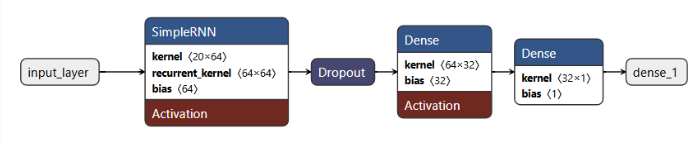
\includegraphics[width=0.75\linewidth]{Figures/RNN1.png} % Assuming this path is correct
%     \caption{Enter Caption}
%     \label{fig:enter-label-rnn1} % Made label unique
% \end{figure}

\begin{figure}[H]
    \centering
    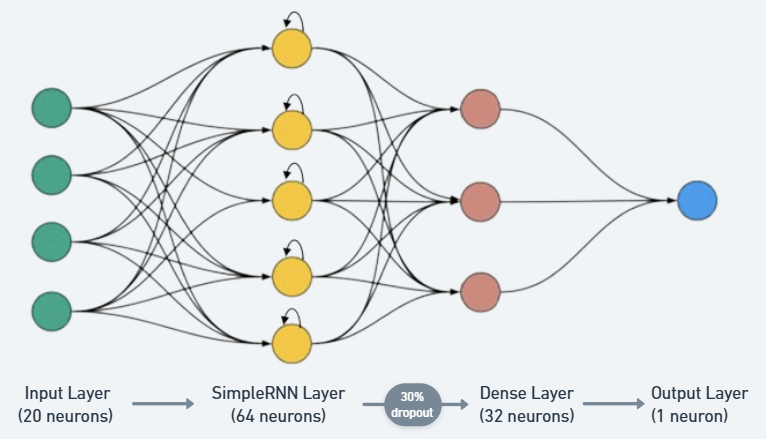
\includegraphics[width=0.75\linewidth]{Figures/RNN2.png} % Assuming this path is correct
    \caption{Enter Caption}
    \label{fig:enter-label-rnn2} % Made label unique
\end{figure}

The model's first layer is a SimpleRNN (64 neurons) that processes sequences, outputting its final hidden state as a consolidated representation. A 20\% dropout layer follows to prevent overfitting. Next, a dense layer (32 neurons, ReLU activation) refines features and reduces dimensionality. The output layer (1 neuron, linear activation) produces the continuous WQI prediction.

Data preprocessing includes robust scaling to mitigate outlier influence and ensure proportional feature contribution. Time-series sequences are generated with a 30-timestep length, enabling the model to use short-term and long-term temporal patterns. The model operates within a Flower federated learning framework for decentralized, privacy-preserving training across clients, safeguarding data and enabling collaborative learning.





\subsection{Secure Application Server Communication}

In our system, the communication between the central configuration server and the Raspberry Pi devices is secured using mutual TLS (mTLS), a protocol that ensures both the client and server authenticate each other before any data is exchanged. Unlike standard TLS, where only the client verifies the server’s identity, mTLS enforces two-way authentication, significantly strengthening security by preventing unauthorized devices from connecting to the system.

  \begin{figure}[H]
    \centering
    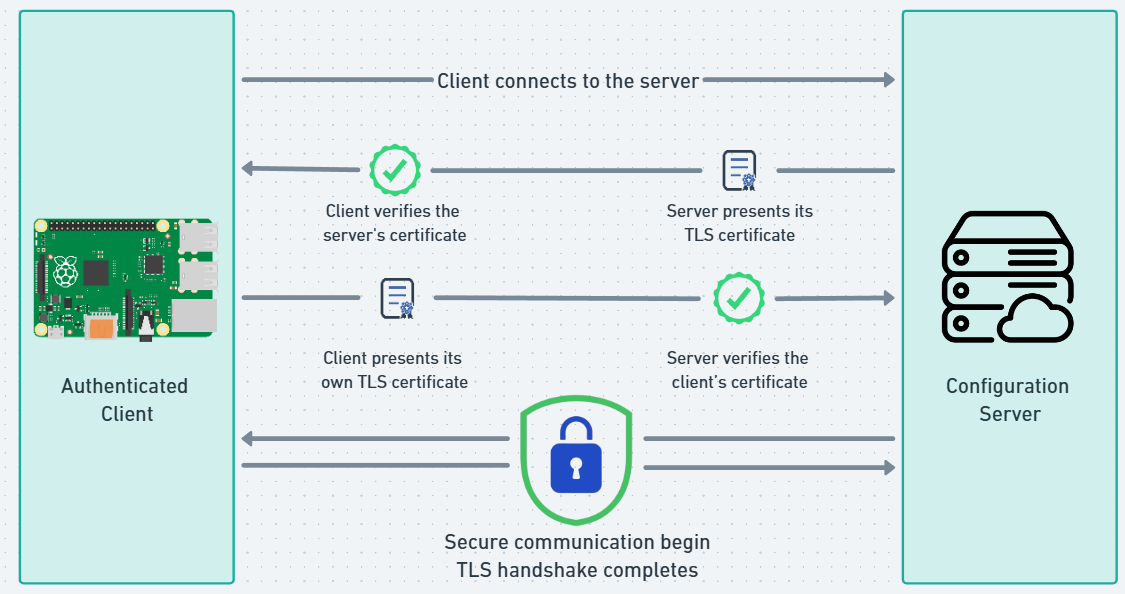
\includegraphics[width=0.75\linewidth]{Figures/mtls2.png}
    \caption{Enter Caption}
    \label{fig:enter-label}
\end{figure}

To establish this secure communication, several cryptographic files are required, including a client certificate for the Raspberry Pi, a corresponding private key, and the certificate authority (CA) certificate used to validate the trust chain. In our solution, the server is fully responsible for generating these certificates. We use a self-signed CA, maintained on the server side, to sign all client certificates.

\begin{figure}[H]
    \centering
    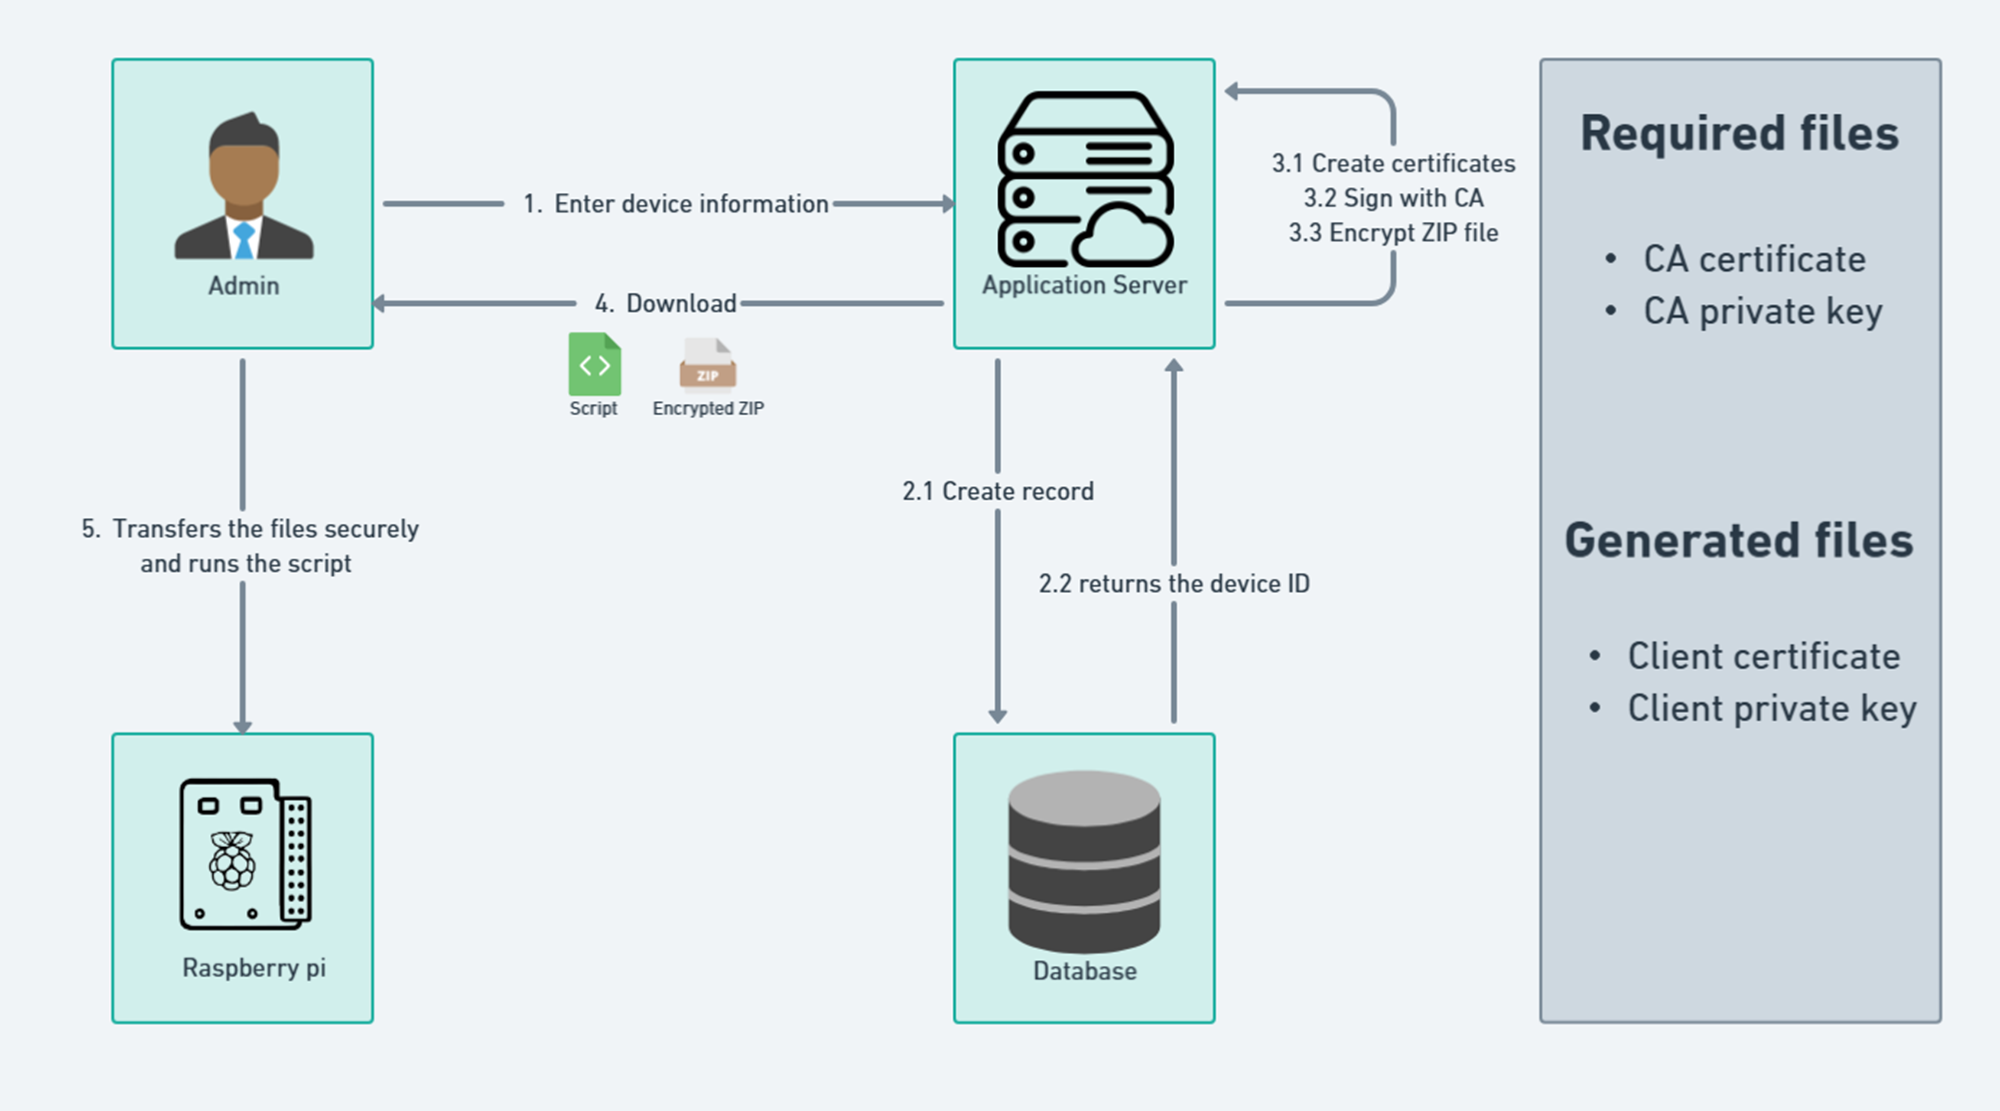
\includegraphics[width=0.75\linewidth]{Figures/security-process.png}
    \caption{Enter Caption}
    \label{fig:enter-label}
\end{figure}

The process begins when the Admin registers a new Raspberry Pi in the system. They must provide relevant information about the device, such as its region and a password. Once submitted, the server creates a new record in the database for the device. The unique ID of this record is then used as the Common Name (CN) in the certificate, ensuring each one is uniquely tied to a specific device.

The server then generates a certificate and private key for the Raspberry Pi and signs the certificate using its internal CA. These files are packaged into a password-protected ZIP archive using the password provided by the Admin. Alongside the archive, the server also generates a shell script that uses the same password and automates the installation of the certificates on the Raspberry Pi. This script simplifies the process for the Admin, allowing them to install the required certificates with minimal effort and ensuring a consistent configuration across devices.

A download link for both the ZIP archive and the installation script is provided to the Admin, who is then responsible for securely transferring them to the appropriate Raspberry Pi device. As these files contain sensitive cryptographic material, it is essential that the Admin uses secure and trusted methods to transfer them. The integrity and confidentiality of these files must be preserved during the transfer to prevent unauthorized access or compromise.



\newpage
\section{Backend and Web Interface}

\subsection{Conception}

\subsubsection{Class Diagram}
\begin{figure}[H]
    \centering
    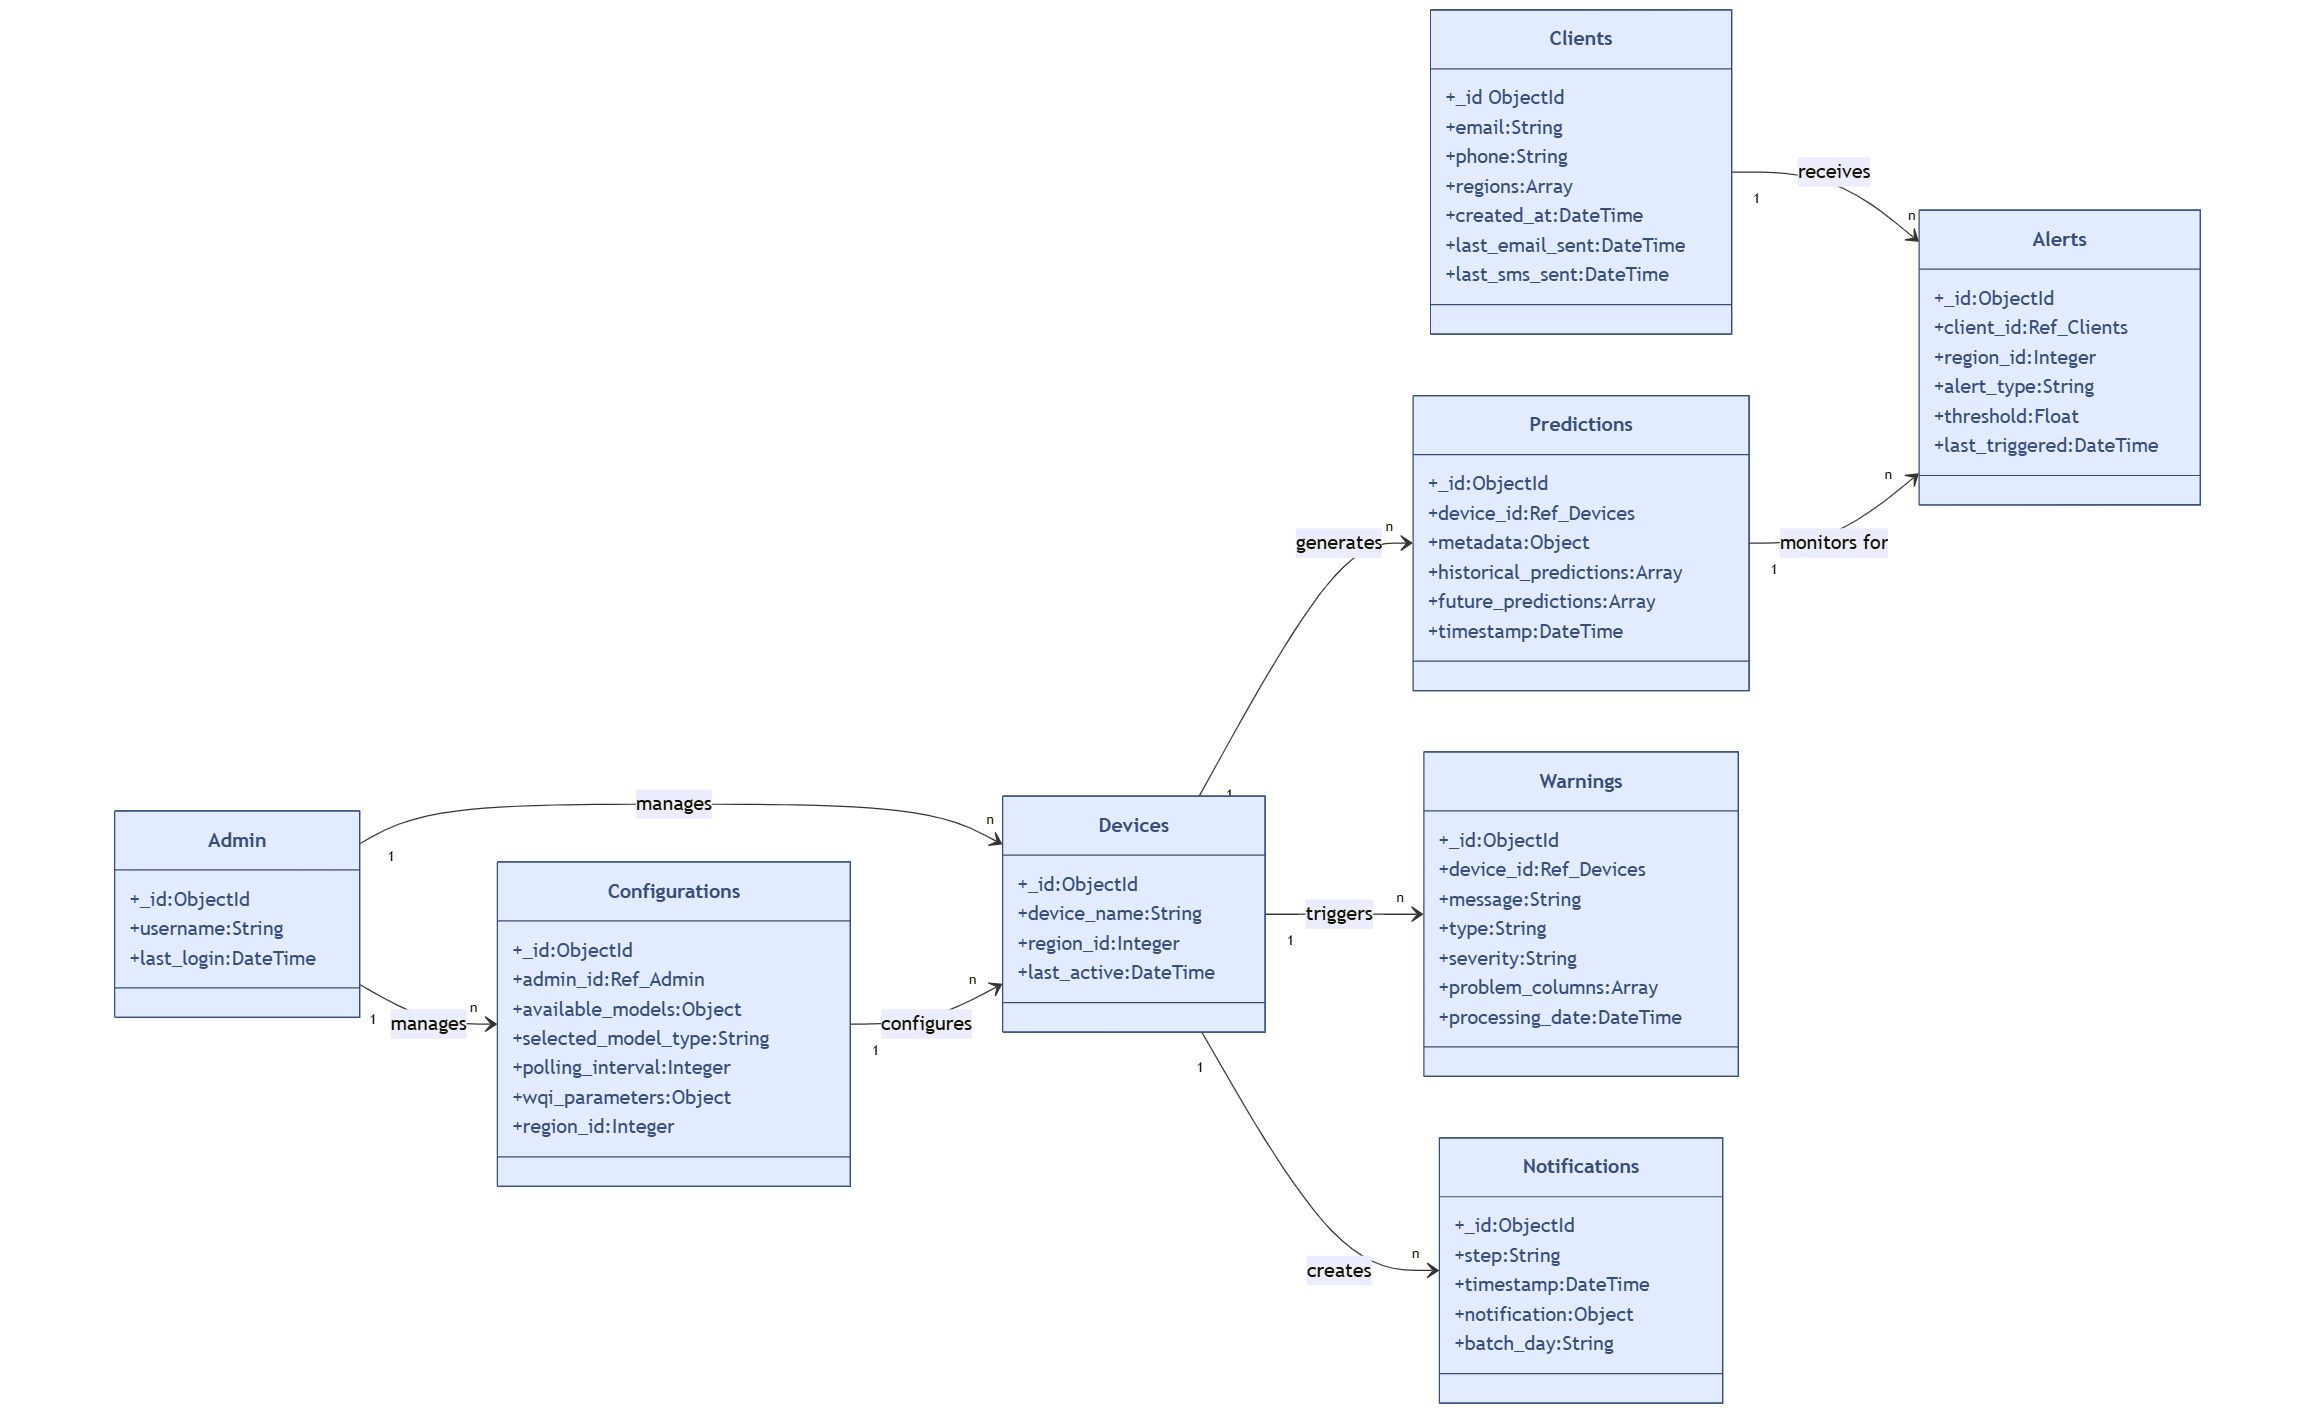
\includegraphics[width=1\linewidth]{Figures/ClasseDia.png}
    \caption{Class Diagram}
    \label{fig:enter-label}
\end{figure}
This class diagram provides an overview of the main entities involved in a monitoring and alert system, along with their relationships. The system includes key classes such as 
 \texttt{Clients}, \texttt{Devices}, \texttt{Admin}, and \texttt{Configurations}, which form the foundation of how users interact with the platform. Each class contains attributes relevant to its role for instance, the \texttt{Clients} class holds contact details and associated regions, while the \texttt{Devices} class represents the hardware responsible for collecting data. The \texttt{Admin} class is responsible for managing configurations and supervising the overall device network.

The relationships between classes illustrate the system's workflow. Devices generate \texttt{Predictions}, which may trigger \texttt{Warnings} and \texttt{Notifications} if certain thresholds are met. \texttt{Alerts} are tied to specific clients, allowing them to receive important updates when necessary. \texttt{Admins} play a central role in managing both devices and configuration settings. Additionally, predictions contribute to alert monitoring, ensuring consistent tracking and analysis of environmental or operational data.
\subsubsection{Application Architecture}
\begin{figure}[H]
    \centering
    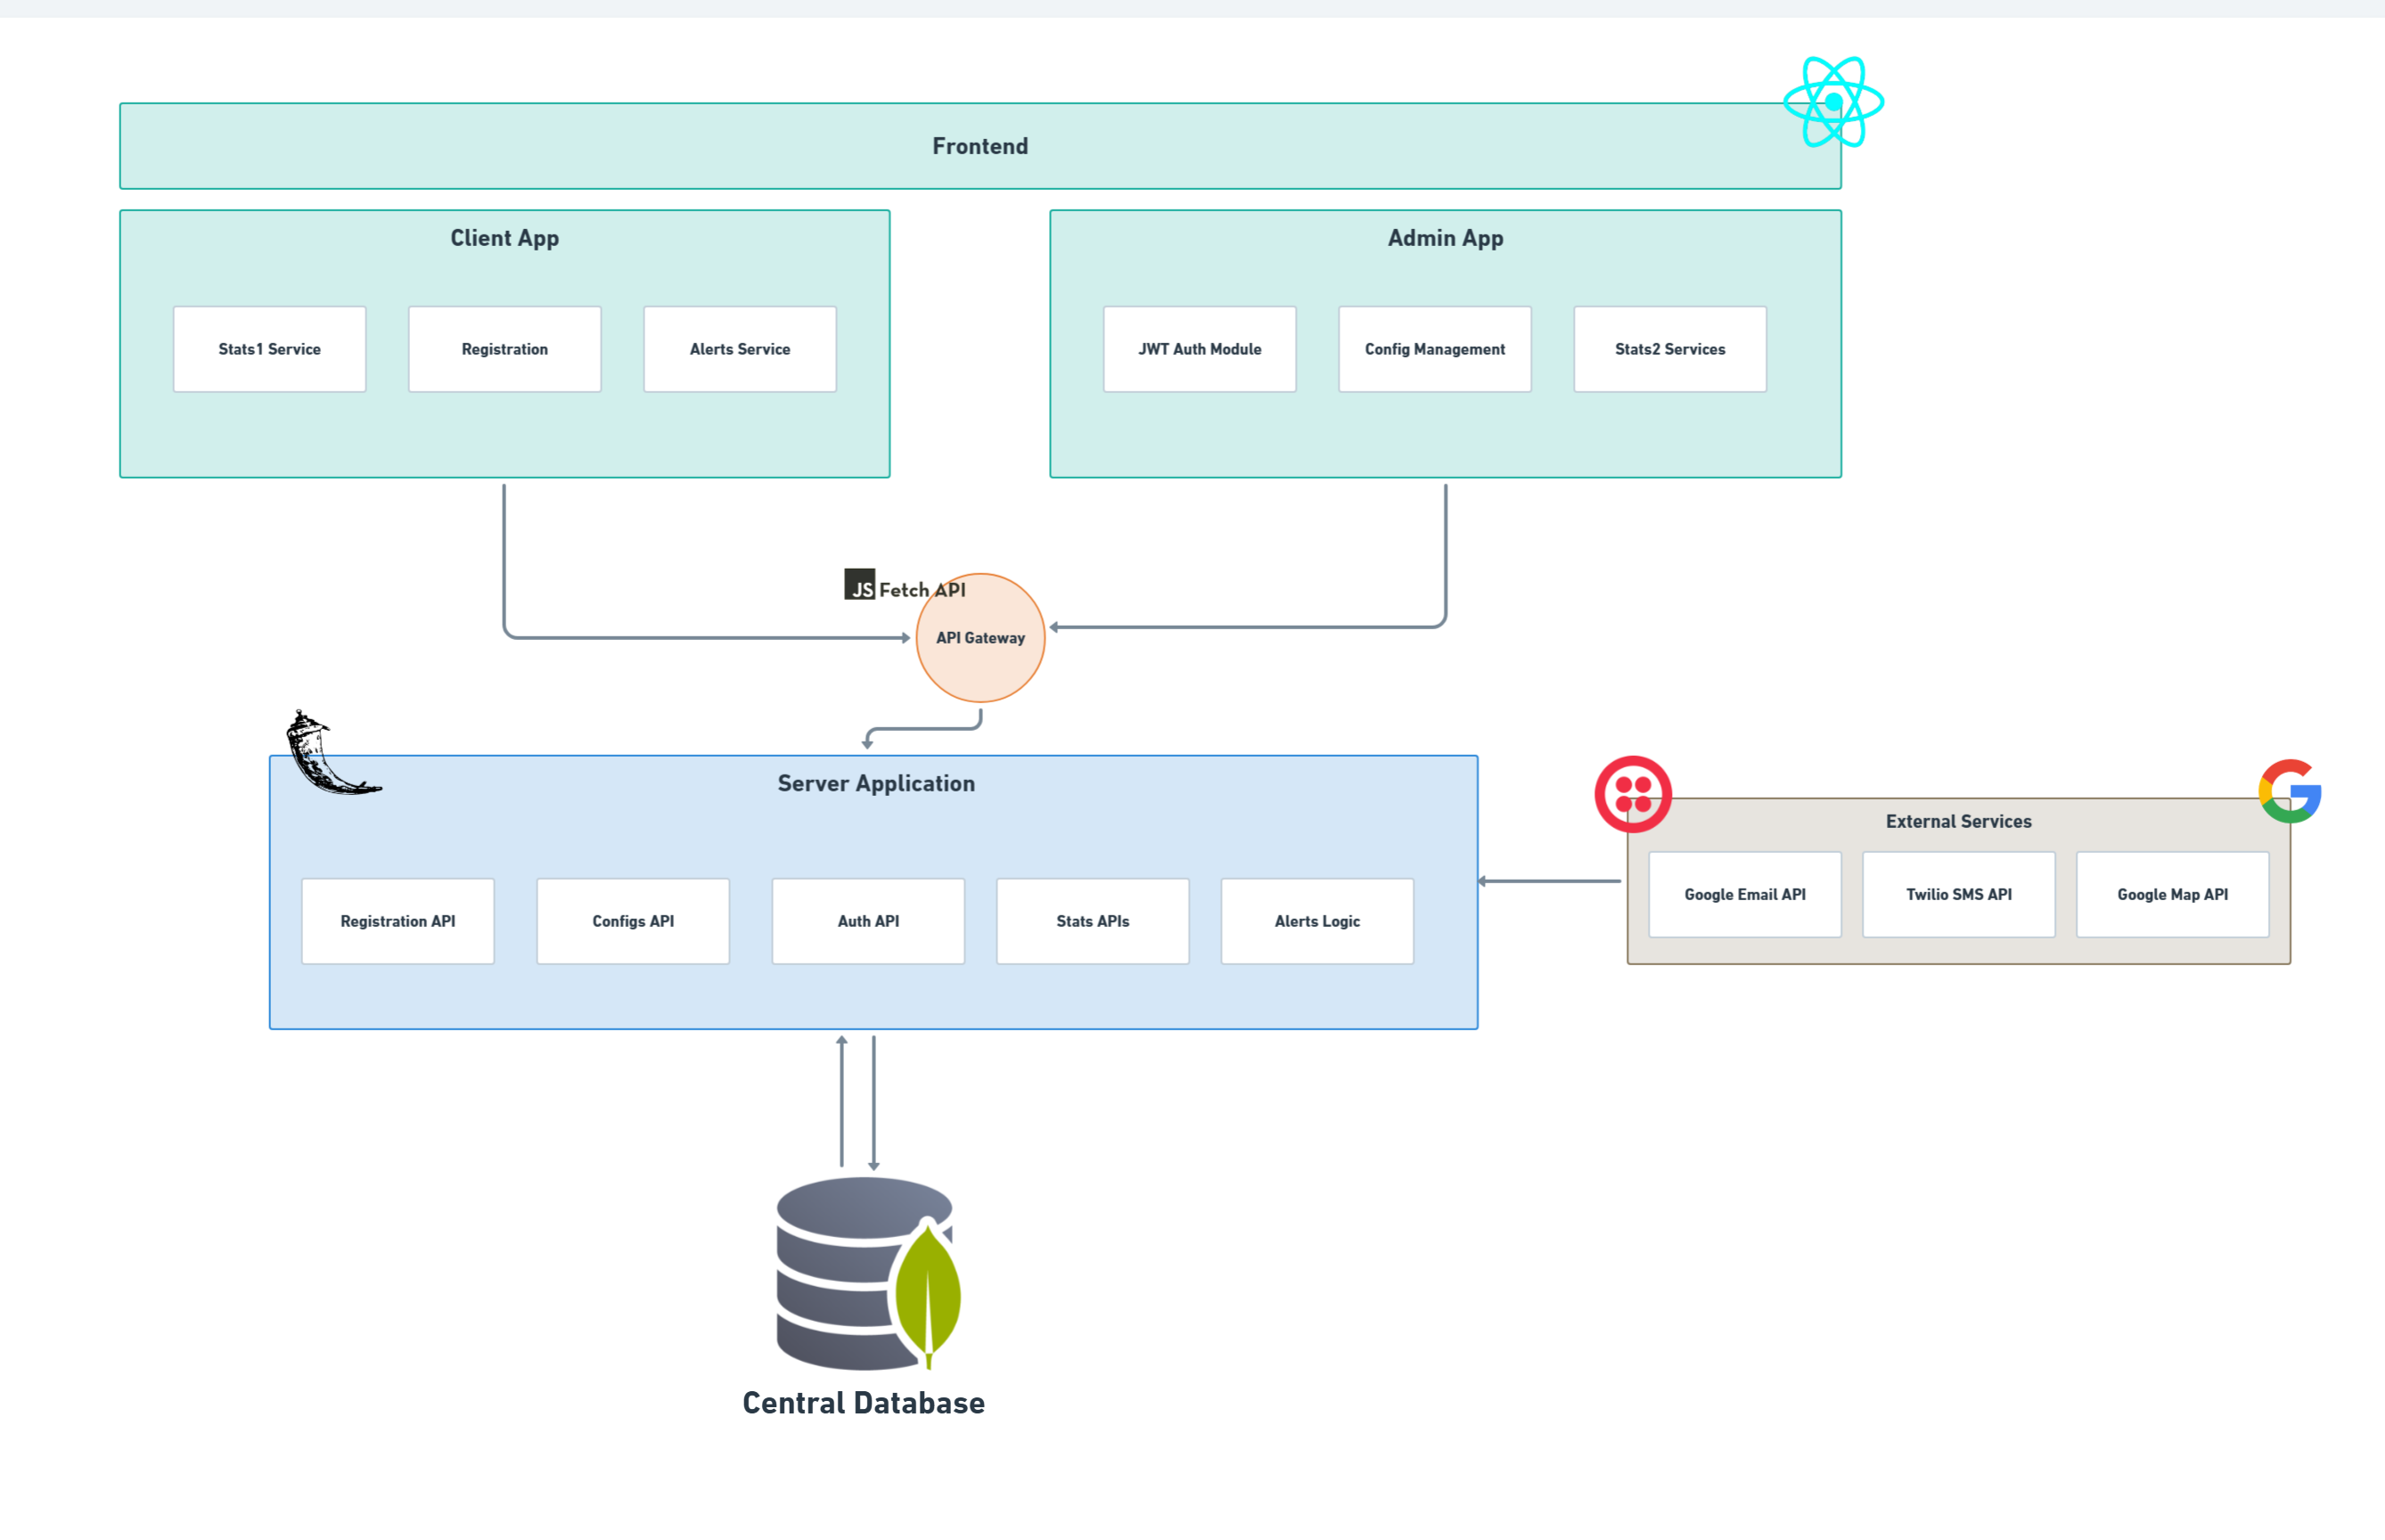
\includegraphics[width=0.75\linewidth]{Figures/ApplicatArch.png}
    \caption{Application Architecture Diagram}
    \label{fig:enter-label}
\end{figure}
The system architecture consists of two distinct React-based frontend applications: one for clients and one for administrators. The client application, built using React and JavaScript with the Fetch API for backend communication, allows users to access and monitor water quality data in major regions across Brussels. Through the \textbf{Stats1 Service}, users can view both historical and predicted Water Quality Index (WQI) values, generated using a time-series model integrated on the backend. An interactive map powered by the Google Maps API displays the current WQI levels for each location. Clients can register using their email, phone number, and select the regions they wish to track. If there is a significant drop in water quality, the system sends alerts via Twilio (for SMS) and Google Email API (for email).

The admin application, also developed with React and securely authenticated via a JWT-based module, provides a detailed operational dashboard for system managers. It interacts with a backend built using Flask, exposing multiple APIs that serve data to the frontend and communicate with Raspberry Pi devices deployed in the field. The dashboard \textbf{Stats2 Service} displays performance statistics such as the number of anomalies detected per day, total data samples, robot distribution by region, and data integrity ratios to help identify malfunctioning devices. It also presents model accuracy metrics related to federated learning (FL), and accuracy readings for pH, conductivity, and other relevant metrics. A configuration management module enables admins to remotely update detection thresholds or cleaning rules on edge devices through Flask APIs. The visualization module avoids raw sensor dumps, instead presenting actionable insights like anomaly alerts and system health indicators.




\subsection{Frontend Dashboard (React.js)}
\subsubsection{Client Application}
\begin{figure}[H]
    \centering
    
\includegraphics[width=0.75\linewidth]{Figures/clientpart1.png}
    \caption{Introduction}
    \label{fig:enter-label}
\end{figure}
This is a section of a webpage. It shows a light blue-themed header with a logo and nav links, a main title about monitoring water quality in Brussels, a short description below it, two buttons ("Explore Regions" and "View Data"), and a water splash on the left side .
\begin{figure}[H]
    \centering
    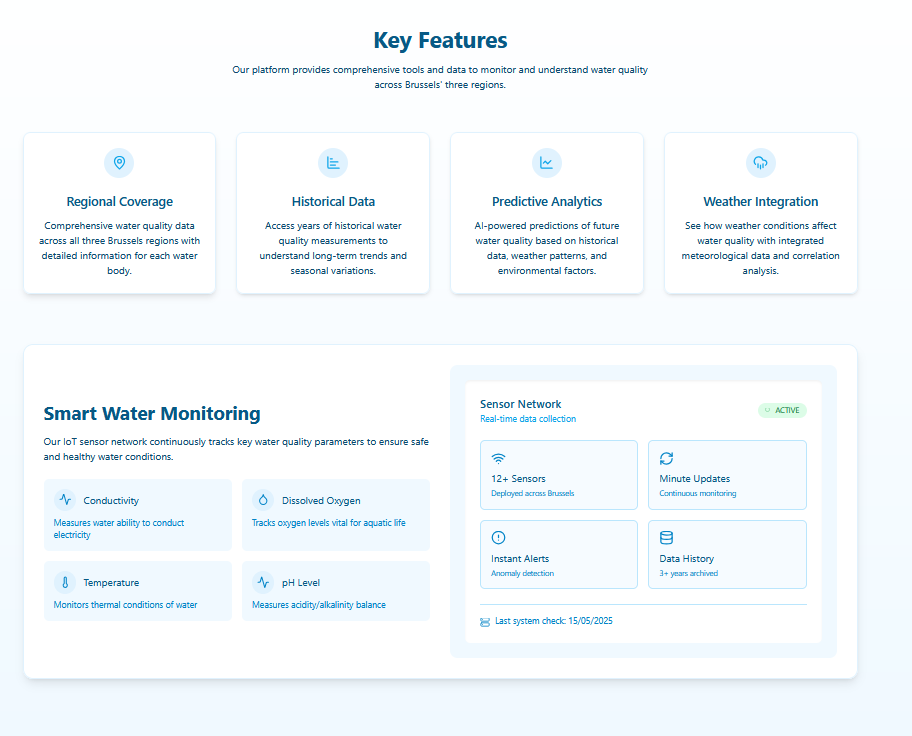
\includegraphics[width=0.75\linewidth]{Figures/clientpart2.png}
    \caption{Key Features and Info}
    \label{fig:enter-label}
\end{figure}
This is a section of a webpage titled Key Features. It presents four main features: Regional Coverage, Historical Data, Predictive Analytics, and Weather Integration each shown in separate cards with icons and short descriptions.

Below, there's a Smart Water Monitoring section describing how an IoT sensor network tracks water quality. It lists parameters like Conductivity, Temperature, Dissolved Oxygen, and pH Level. On the right, a card labeled Sensor Network shows real-time data features such as sensor count, update frequency, alerts, and data history.
\begin{figure}[H]
    \centering
    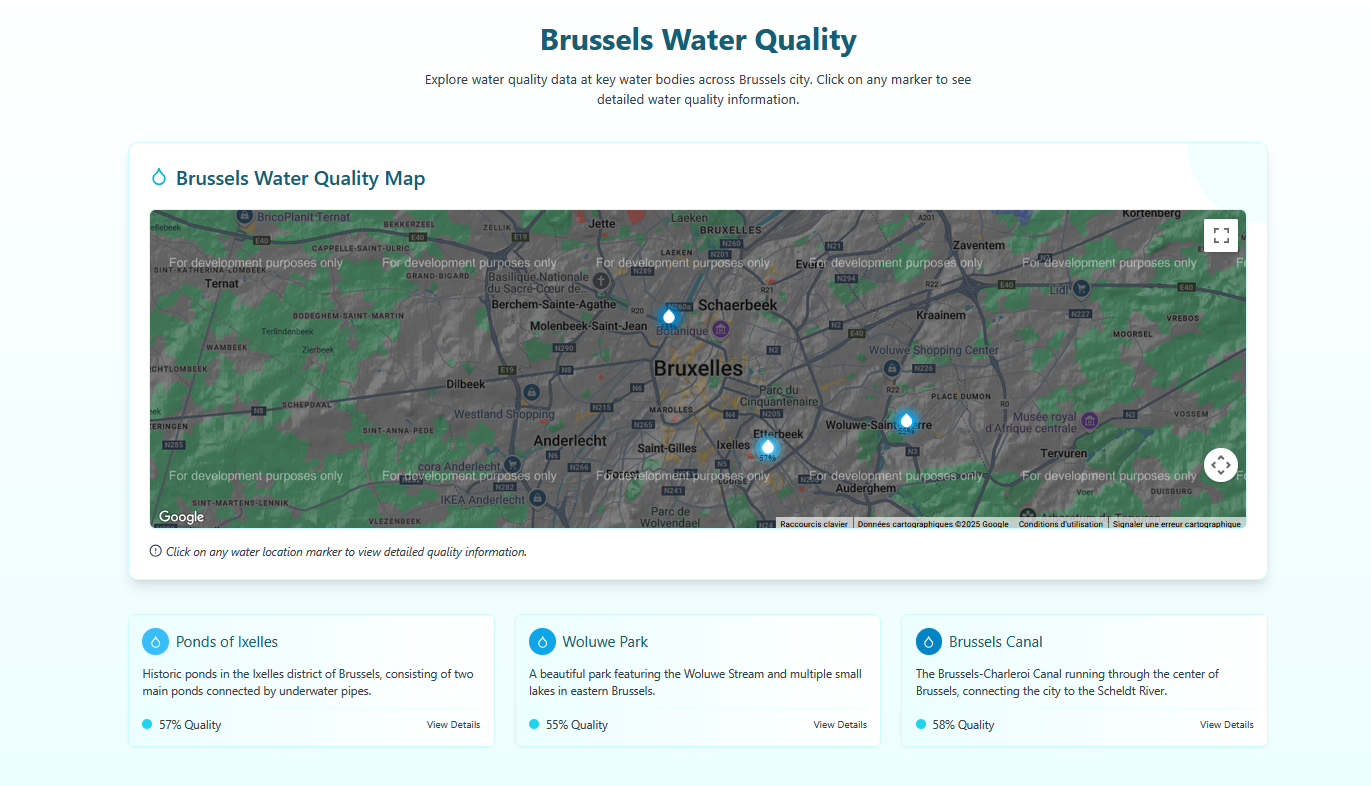
\includegraphics[width=0.75\linewidth]{Figures/clientt4.png}
    \caption{Map Feature Part 1}
    \label{fig:enter-label}
\end{figure}
The page presents an interactive map interface for Brussels water quality, using clickable pin markers and corresponding cards below the map to display information. When a user clicks on a pin or a card, a modal appears, and selecting a card also zooms the map to that specific location.
\begin{figure}[H]
    \centering
    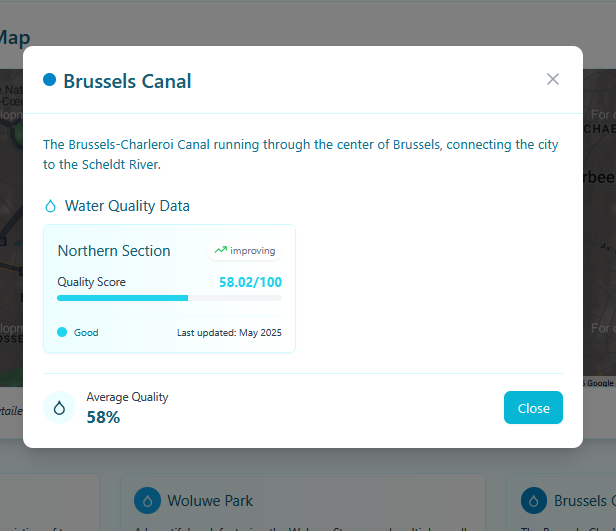
\includegraphics[width=0.75\linewidth]{Figures/clientt5.png}
    \caption{Map Feature Part 2}
    \label{fig:enter-label}
\end{figure}
When the client clicks on a specific marker on the map or selects one of the location cards, a modal is triggered. This modal presents detailed information about the selected location within one of the regions. The modal includes the Water Quality Index (WQI), the historical trend of water quality, and a brief contextual description of the location.
\begin{figure}[H]
    \centering
    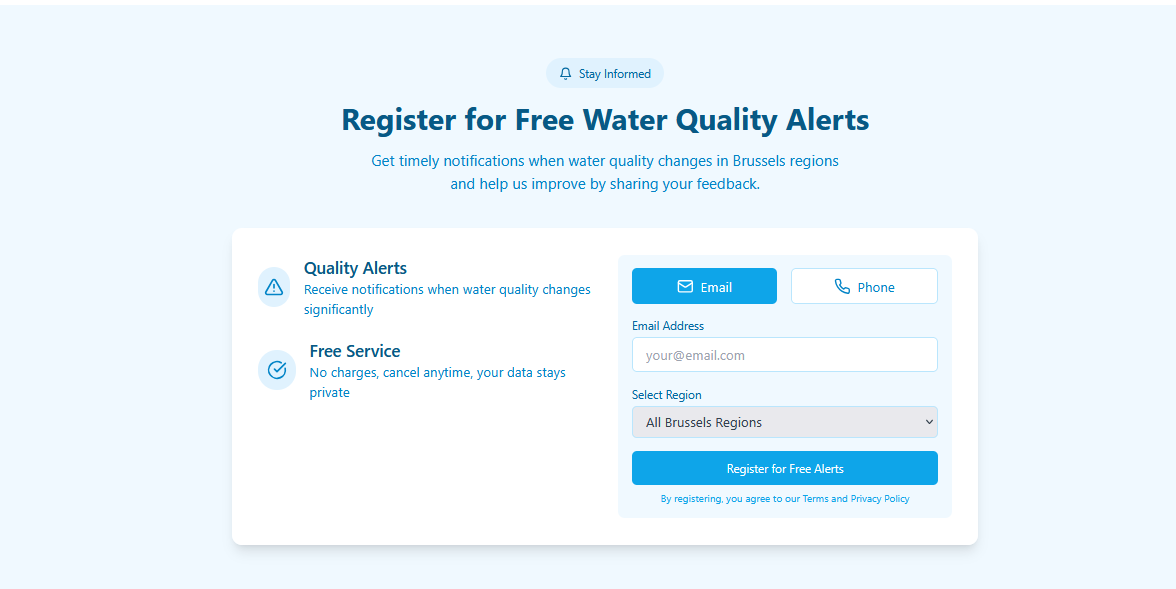
\includegraphics[width=0.75\linewidth]{Figures/clientpart8.png}
    \caption{Registration}
    \label{fig:enter-label}
\end{figure}
This registration form allows clients to subscribe to free water quality alerts via email, phone. Users can specify which Brussels regions they want to monitor. The system will then send timely notifications through Twilio for SMS and the Google Email API whenever a significant drop in water quality is detected in their selected regions, keeping them informed in real-time without constant app monitoring.
\begin{figure}[H]
    \centering
    
\includegraphics[width=0.75\linewidth]{Figures/Clientpartfinal.png}
    \caption{Post-Registration}
    \label{fig:enter-label}
\end{figure}
Upon successful registration, the user receives confirmation that they will now receive water quality alerts for their selected regions. A confirmation email is also sent to the provided address, ensuring the user is aware of their subscription and can expect to receive timely notifications about significant water quality changes.
\subsubsection{Admin Application}
\begin{figure}[H]
    \centering
    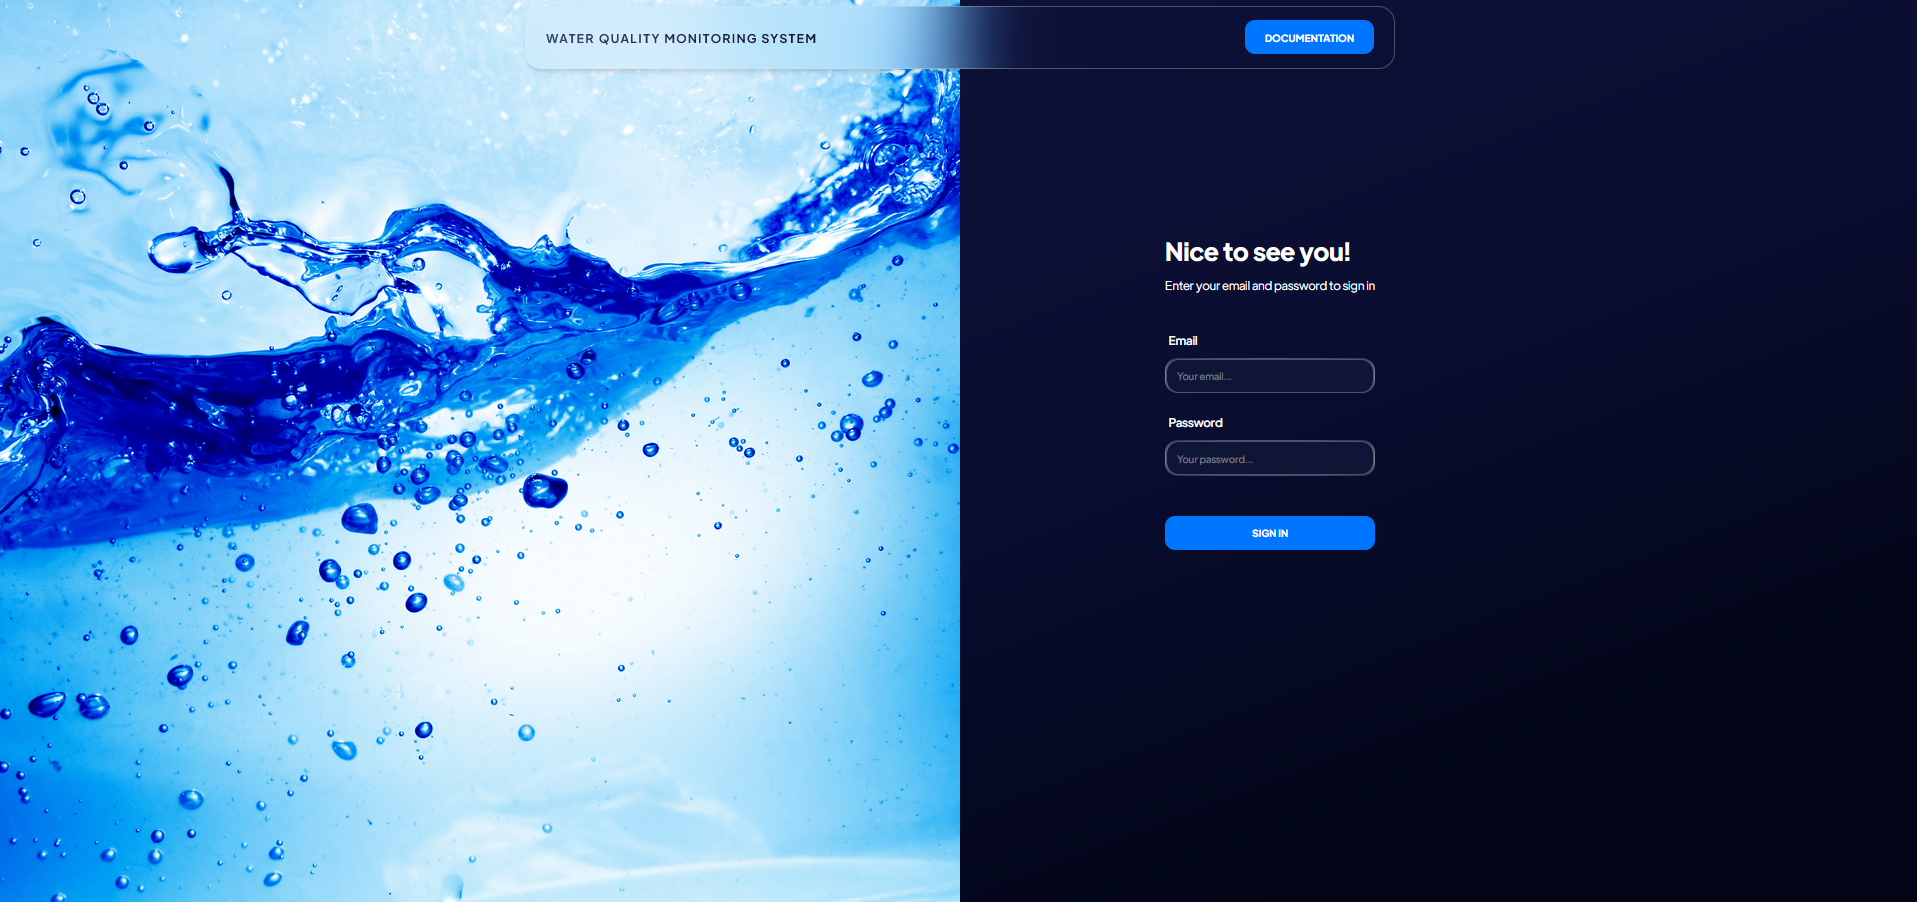
\includegraphics[width=0.75\linewidth]{Figures/admin1.png}
    \caption{Authentification Page}
    \label{fig:enter-label}
\end{figure}
The authentication page for the Water Quality Monitoring System features a straightforward login form, requesting the user's email and password. Notably, the system employs JWT  for secure user authentication. JWT ensures robust session management by generating encrypted tokens upon successful login.
\begin{figure}[H]
    \centering
    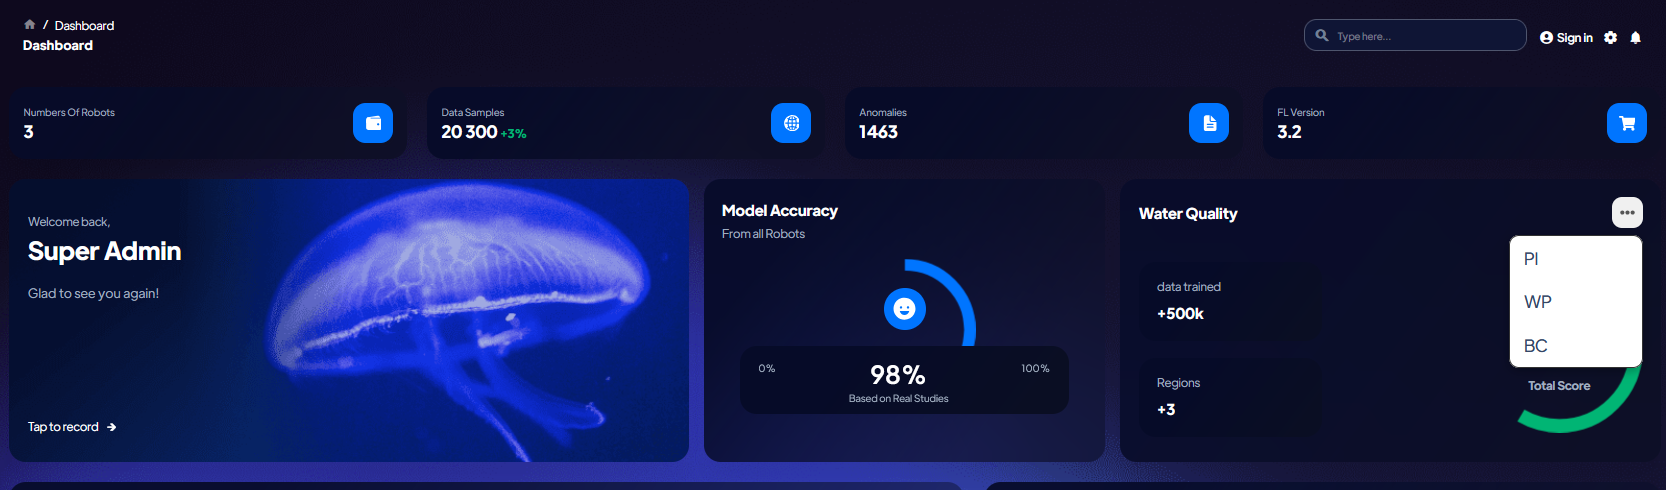
\includegraphics[width=0.75\linewidth]{Figures/admin2.png}
    \caption{Dashboard part 1}
    \label{fig:enter-label}
\end{figure}
This dashboard provides a unified view of business and environmental metrics, featuring admin analytics, service performance, and water quality data. Key sections include  number of active devices, model accuracy scores, and regional WQI trends with color-coded visuals. While effectively presenting diverse data, adding interactive elements could enhance usability.
\begin{figure}[H]
    \centering
    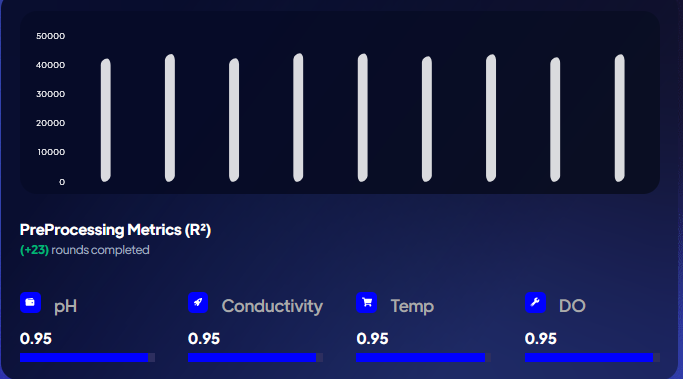
\includegraphics[width=0.75\linewidth]{Figures/admin3.png}
    \caption{Dashboard part 2}
    \label{fig:enter-label}
\end{figure}
This chart adopts a structured and minimalistic design to communicate model performance. The upper section features vertical bars that track outliers over time, visualizing monthly anomaly trends. The lower section presents accuracy scores across key water quality parameters, reflecting the strength of data cleaning models.

\begin{figure}[H]
    \centering
    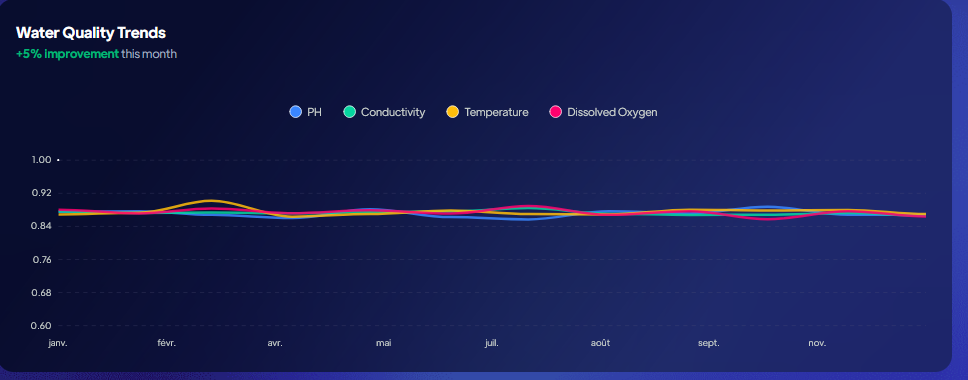
\includegraphics[width=0.75\linewidth]{Figures/dashboard4.png}
    \caption{Dashboard part 3}
    \label{fig:enter-label}
\end{figure}
This chart shows monthly trend lines for four water quality metrics. It displays percentage change data and tracks measurements across an eight-month period. The visualization uses a shared scale to compare the parameters, with time labels along the horizontal axis. A percentage indicator appears at the top. The chart presents the data clearly without interactive elements.
\begin{figure}[H]
    \centering
    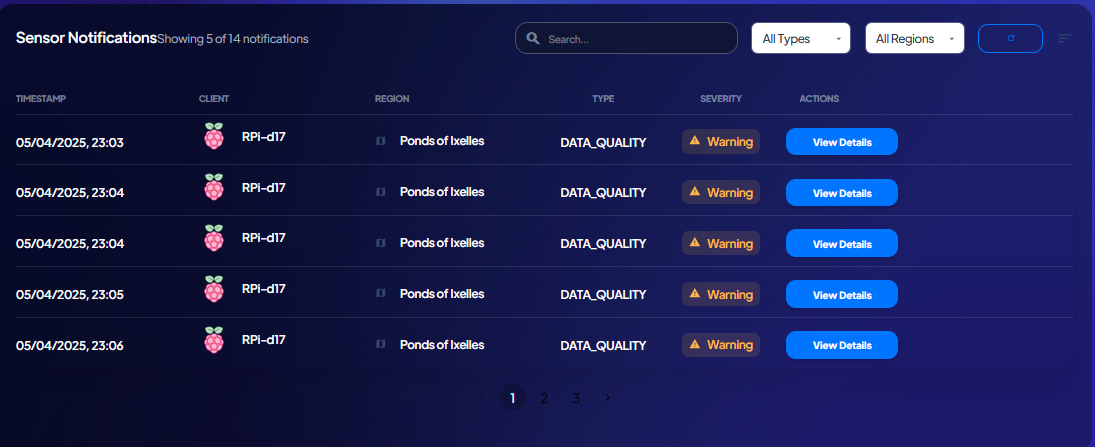
\includegraphics[width=0.75\linewidth]{Figures/admin5.png}
    \caption{dashboard part 4}
    \label{fig:enter-label}
\end{figure}
The interface displays a filterable notification log showing sensor alerts, including timestamps, locations, error types, and severity levels. It presents five entries for every page with options to sort by multiple columns and a search function. The visible alerts primarily show processing errors from one sensor location, with one data quality warning. Each entry includes an action button ("View Details") for further investigation.
\begin{figure}[H]
    \centering
    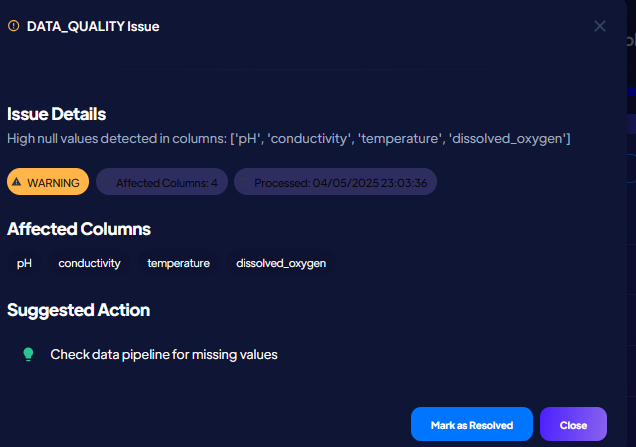
\includegraphics[width=0.7\linewidth]{Figures/admin8.png}
    \caption{dashboard part 5}
    \label{fig:enter-label}
\end{figure}

The interface displays a detailed data quality alert, showing affected measurement columns with null values. It includes the detection timestamp, severity level (warning), and recommended troubleshooting steps. The layout presents the information clearly with column headers, a suggested action prompt, and resolution options ("Mark as Resolved"/"Close").

\begin{figure}[H]
    \centering
    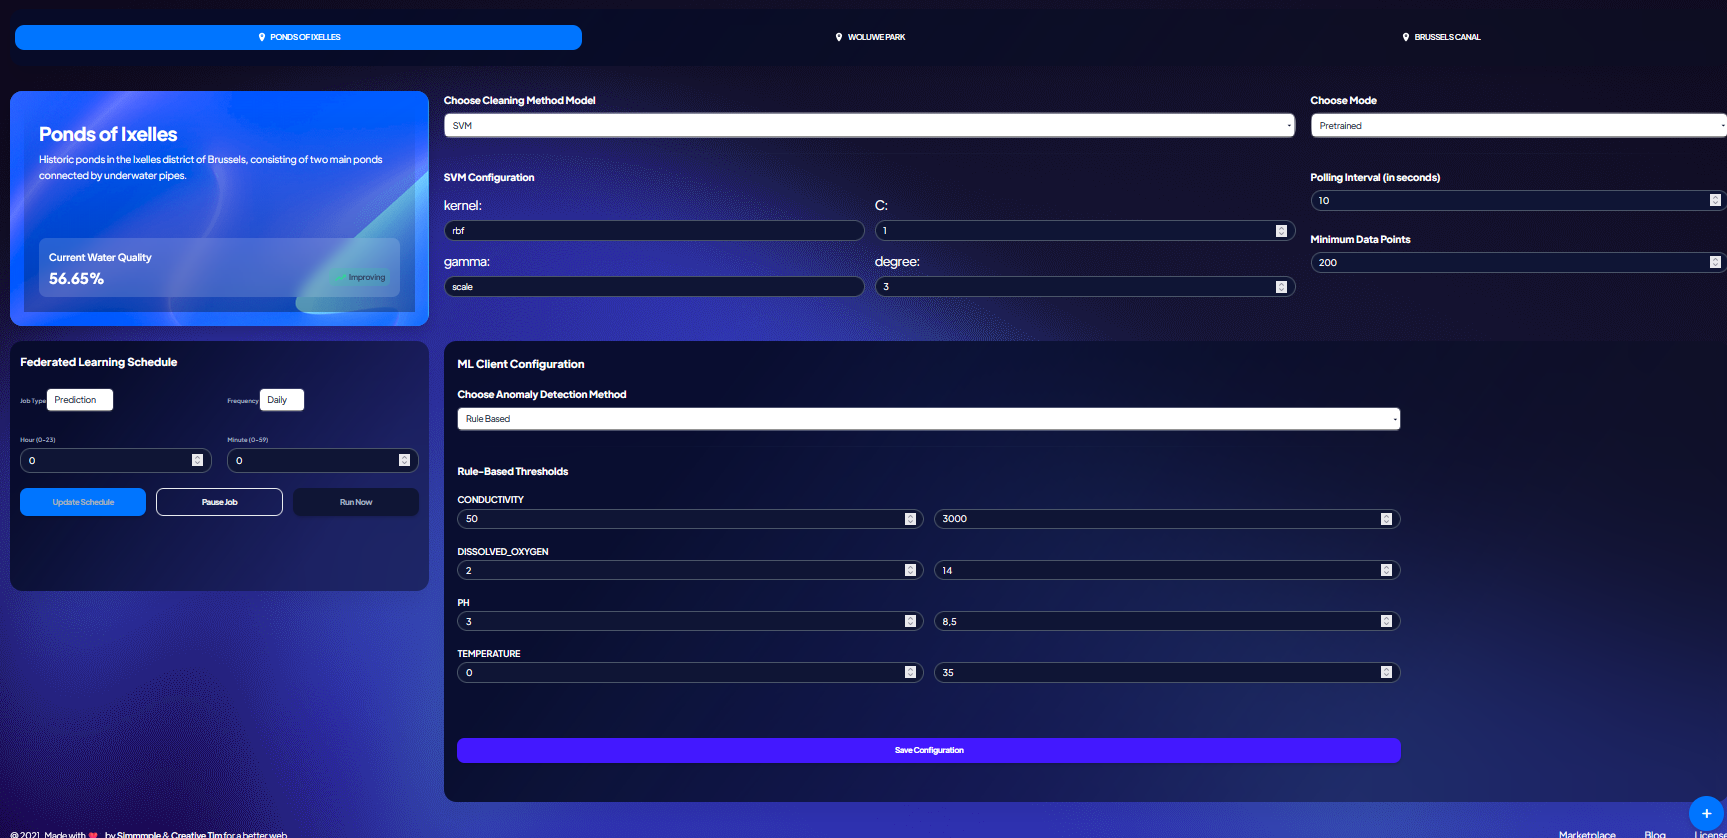
\includegraphics[width=0.75\linewidth]{Figures/configpage.png}
    \caption{Configurtion Page}
    \label{fig:enter-label}
\end{figure}


This Config panel provides an admin interface for comprehensively configuring a monitoring system., admin can select a "Cleaning Method Model" from a dropdown list (like SVM, KNN, RandomForest) and then input specific hyperparameter values for the chosen model into corresponding text fields or dropdowns. Similarly, for "ML Client Configuration," admin can choose an "Anomaly Detection Method" from a list (such as Rule-Based, IQR, Decision Tree). If "Rule-Based" is selected, the interface presents input fields to define numerical upper and lower thresholds for various sensor readings like conductivity, dissolved oxygen, pH, and temperature. If another method like Decision Tree were selected, different relevant parameter input fields would appear.
The interface also allows users to set general operational parameters like the "Polling Interval" and "Minimum Data Points" through numerical input fields, and select an operating "Mode" from a dropdown. For "Federated Learning Schedule," admin can select a "Job Type" (Prediction or Training), a "Frequency" (like Weekly, Monthly), and input specific times using hour and minute fields. Buttons for "Update Schedule," "Pause Job," and "Run Now" trigger corresponding backend actions. Finally, a "Save Configuration" button applies all the settings configured across these sections.

\begin{figure}[H]
    \centering
    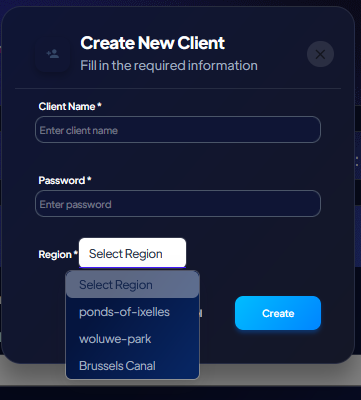
\includegraphics[width=0.5\linewidth]{Figures/create1.png}
    \caption{ Create Client Modal}
    \label{fig:enter-label}
\end{figure}
The interface shows a form for creating new device record, with required fields for name, password, and region selection. It includes a dropdown menu for choosing from predefined water monitoring locations. 
\begin{figure}[H]
    \centering
    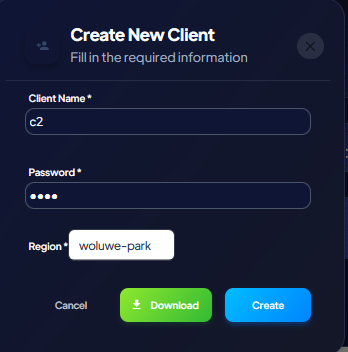
\includegraphics[width=0.5\linewidth]{Figures/create2.png}
    \caption{Enter Caption}
    \label{fig:enter-label}
\end{figure}

The interface displays a device creation form with fields for name, password, and region selection. After filling the form, a download button appears to retrieve security files (client.crt, client.key, ca.crt) packaged in a RAR archive.



\newpage

\section*{Conclusion}

This chapter comprehensively detailed the practical construction of the Federated Learning system for water quality monitoring, successfully translating architectural designs into a functional prototype. Key software components were developed and integrated, including mechanisms for data simulation, a robust preprocessing pipeline featuring anomaly detection and model-based cleaning, and the core federated learning workflow. Advanced analytical capabilities were implemented through dedicated feature engineering and the development of a Recurrent Neural Network model for water quality prediction. Security was a central focus, with mTLS and TLS protocols integrated to ensure secure communication across the system. Furthermore, user-facing client and administrator web interfaces were built using React.js with a Flask backend, providing essential tools for interaction, monitoring, and configuration. The successful amalgamation of these diverse elements into a working system demonstrates the viability of creating a sophisticated, privacy-preserving, and decentralized monitoring solution, thereby laying a solid groundwork for subsequent real-world testing and continued refinement.

\pagebreak
\chapter{Results and Discussion}
\label{chap:results}
\section*{Introduction}
This chapter presents and discusses the results from the implementation and evaluation of the Federated Learning (FL) system for Water Quality Monitoring (WQM) in distributed environments, as designed in Chapter IV. The primary objective is to provide empirical evidence of the system's functionality, performance, and overall viability. The chapter systematically evaluates the local data preprocessing pipeline deployed on client devices. Subsequently, it delves into the core of the system: the effectiveness and convergence characteristics of the federated learning model for Water Quality Index (WQI) prediction. Following this, it presents the results from testing the client and admin web applications, including their usability and the functionality of secure communication protocols. The findings are then contextualized against the project's initial objectives, highlighting the system's strengths, identifying potential limitations, and considering the implications for real-world deployment and future research directions.

\newpage

\section{Data Preprocessing Evaluation}
\subsection{Testing Frameworks Utilized}

\begin{figure}[h]
    \centering
    
\includegraphics[width=0.15\linewidth]{Figures/pytest.png}
    \caption{Pytest Logo}
    \label{fig:enter-label}
\end{figure}
Pytest is a widely used testing framework for Python, known for its simple syntax, extensive plugin support, and ability to handle complex testing scenarios efficiently. In this evaluation, Pytest version 8.3.5 was employed to validate the preprocessing pipeline’s functionality, focusing on utility services, data processing modules, data persistence, configuration management, and client scripts.

\subsection{Test Suite Summaries and Key Validations}
The data preprocessing pipeline deployed on each Raspberry Pi client is a critical component in ensuring data quality prior to federated training. This section presents the testing and key findings, and detailed analysis of the preprocessing pipeline’s performance under simulated operational conditions.

The objective of this evaluation phase was to verify the correct integration and functionality of key components within the Water Quality Monitoring System. The testing suite targeted utility services, data processing modules, data persistence mechanisms, configuration management, and client-side scripts. Pytest version 8.3.5 was employed in a Python 3.11.2 environment, with a total execution time of 4.11 seconds.

A suite of 39 automated tests was executed, all of which successfully passed. The distribution and results of these tests are summarized in Figure \ref{fig:preprocessing-tests}.

\begin{figure}[h]
    \centering
    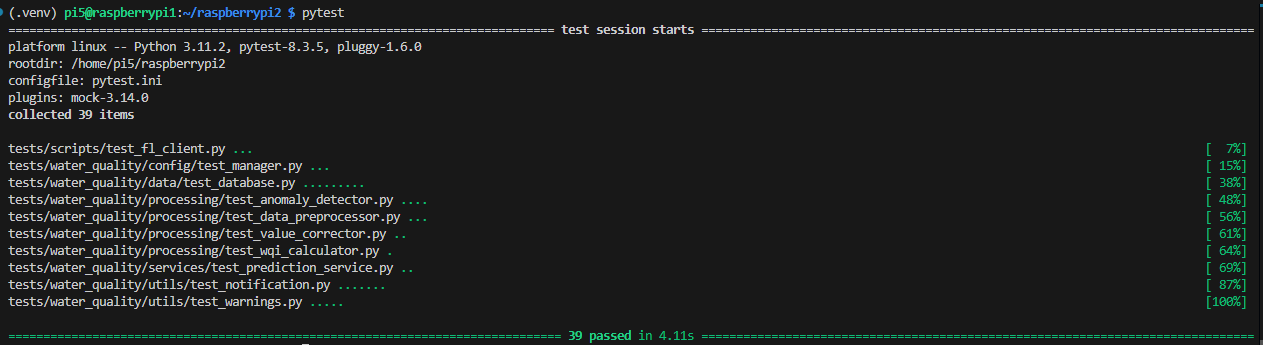
\includegraphics[width=1\linewidth]{Figures/preprecessing_tests.png}
    \caption{Enter Caption}
    \label{fig:preprocessing-tests}
\end{figure}

Utility services, including the NotificationService and WarningSystem, were validated for singleton patterns, initialization routines, and error handling. The data processing pipeline’s reliability was further demonstrated through specific tests that evaluated the AnomalyDetector’s accuracy in detecting outliers using IQR and rule-based methods. Additionally, the ValueCorrector’s integration with ModelManager was assessed for its capacity to correct flagged anomalies based on model predictions. Furthermore, the WQICalculator’s ability to adaptively adjust its configuration and correctly classify water quality labels based on dynamic threshold updates was validated.

Data integrity during retrieval and incremental updates was confirmed through tests focused on data type verification and consistency during the validation phase.

The performance of configuration management and client-side scripts was evaluated for their ability to manage configurations and preprocess data effectively. The ConfigManager was tested for its ability to merge remote configurations with default settings, while client scripts were validated for their successful execution of feature engineering steps without introducing NaN values or data inconsistencies.
 
\section{Water Quality Index Prediction Model Evaluation}
\label{sec:wqi_model_evaluation}
The core of the system's predictive capability lies in its ability to accurately forecast the Water Quality Index (WQI). This section details the two-stage process undertaken: first, a comprehensive centralized machine learning exploration to identify an optimal model and feature set; and second, the implementation and preliminary evaluation of the selected model within the federated learning environment.
\subsection{Centralized Model Selection: Experimental Setup}
\label{ssec:centralized_setup}
The WQI prediction model's performance was initially evaluated using a structured centralized approach involving historical water quality cleaned datasets.
\begin{itemize}
\item \textbf{Initial Feature Engineering:} A comprehensive set of 63 features was engineered from the base data (pH, temperature, dissolved oxygen, conductivity, and WQI), including temporal markers, rolling statistics, percentage changes, and interaction terms.
\item \textbf{Iterative Feature Reduction:} Several iterations were performed where subsets of these engineered features were removed based on their correlation with the target (WQI) and domain knowledge, aiming to find an optimal feature set that balances model performance and complexity.
\item \textbf{Model Architecture Exploration:} Using a selected "best" feature set, different configurations of a SimpleRNN model were tested to observe the impact of network depth and width.
\item \textbf{Evaluation Metrics:} Model performance was primarily assessed using Mean Absolute Error (MAE) and Root Mean Squared Error (RMSE) on the original WQI scale. Training MAE was recorded to monitor model fitting.
\item \textbf{Validation Strategy:} Time Series Cross-Validation (TSCV) with 3 splits was used on the development dataset to get the validation metrics. A final set of hold-out tests (15\% of the sequenced data) was used for the evaluation of the trained model from each iteration/architecture.
\end{itemize}
\subsection{Centralized Model Evaluation: Iterative Feature Reduction and Architecture Performance}
\label{ssec:centralized_performance}


\subsubsection*{Summary and Selection for Federated Learning}
\label{sssec:centralized_summary_selection}
A comparative summary of all centralized iterations and architecture explorations is presented in Table \ref{tab:model_performance_comparison}.

\begin{figure}[H]
    \centering
    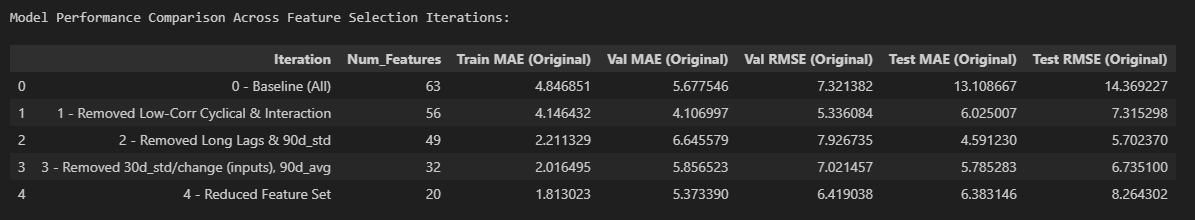
\includegraphics[width=0.75\linewidth]{Figures/feature_selection.png}
    \caption{Feature Selection Results}
    \label{fig:enter-label}
\end{figure}

To begin optimizing our model, we first applied extensive feature engineering to generate a comprehensive set of 63 features, capturing cyclical patterns, lagged values, and statistical indicators, in order to maximize the model’s ability to learn from historical trends. However, to address potential redundancy and overfitting, we adopted a step-by-step feature selection strategy based on domain knowledge and correlation analysis. In the baseline configuration with all 63 features, the model yielded a train MAE of 4.85, validation MAE of 5.68, and a high test MAE of 13.11, clearly indicating overfitting. By gradually removing less informative features, we saw significant improvements: at 56 features, test MAE dropped to 6.03; at 49 features, we observed the lowest test MAE of 4.59, albeit with a rise in validation error; a 32-feature set yielded more balanced performance (test MAE: 5.79); and finally, with just 20 features, we achieved a strong balance between performance and complexity, with a train MAE of 1.81, validation MAE of 5.37, and test MAE of 6.38. This final configuration offered the best compromise between model generalization, simplicity, and reduced risk of overfitting.
\begin{figure}[H]
    \centering
    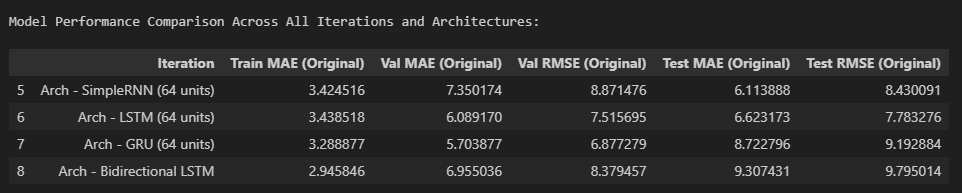
\includegraphics[width=0.75\linewidth]{Figures/model_selection.png}
    \caption{Enter Caption}
    \label{fig:enter-label}
\end{figure}
Using this optimized feature set, we then evaluated different recurrent neural network architectures, including SimpleRNN, LSTM, GRU, and Bidirectional LSTM, each with 64 units. While deeper models like GRU and BiLSTM delivered slightly strong results, our decision prioritized not only performance but also computational efficiency, as our target deployment environment is a Raspberry Pi.

The SimpleRNN model achieved a train MAE of 3.42 and a test MAE of 6.11, with reasonable RMSE values. Although there is a modest gap between training and test errors  indicating slight overfitting  SimpleRNN was selected as the most appropriate architecture. Its simplicity, low resource consumption, and solid performance make it an ideal fit for our real-world deployment scenario, where balancing accuracy with hardware limitations is critical.
% \begin{table}[h]
%     \centering
%     \caption{Model Performance Comparison Across Feature Selection Iterations and Architectures (Centralized Training).}
%     \label{tab:model_performance_comparison}
    % \begin{tabular}{lcccccc} % Adjust column alignment as needed
    % \toprule
    % Iteration/Architecture & Num\_Features & Train MAE & Val MAE & Val RMSE & Test MAE & Test RMSE \\
    % \midrule
    % 0 - Baseline (All) & 63 & 0.8268 & 1.7333 & 2.1483 & 1.4647 & 1.5446 \\
    % ... (rest of your table data) ... \\
    % Arch C - Stacked RNN & 20 & 2.1673 & 1.7750 & 2.4826 & 1.7972 & 2.2231 \\
    % \bottomrule
    % \end{tabular}
    % \includegraphics[width=1\linewidth]{Figures/your_table_image.png} % << USE THIS IF YOU HAVE AN IMAGE OF THE TABLE
    % If you don't have an image, you'll need to manually create the LaTeX table structure above.
% \end{table}

The centralized model evaluation (Table \ref{tab:model_performance_comparison}) revealed that the baseline model (Iteration 0, 63 features) provided the best MAE on the hold-out test set (1.4647). However, the Stacked RNN (Architecture C) using the curated set of 20 features (from Iteration 4) achieved a highly competitive test MAE of 1.7972. Given the objectives of a federated system where model simplicity and reduced data footprint are advantageous, Architecture C with 20 features (Iteration 4) was selected as the primary candidate for implementation in the federated learning environment. The baseline model (Iteration 0) was also considered for FL implementation to provide a comparative benchmark.

\subsection{Federated Learning Model Implementation and Preliminary Results}
\label{ssec:fl_results}
Following the centralized model selection process, the chosen model configurations were implemented within a simulated federated learning environment using the Flower framework (version X.Y.Z). The simulation involved 3 clients, each provisioned with a distinct, non-IID partition of the historical dataset, processed according to the feature engineering pipeline detailed in Chapter IV. The Federated Averaging (FedAvg) strategy was employed for model aggregation by the central FL server over [e.g., 10] communication rounds. Each client performed [e.g., 5] local epochs of training per round.

\subsubsection{Federated Model with Iteration 4 Features and Architecture C (20 Features, Stacked RNN)}
\begin{figure}[H]
    \centering
    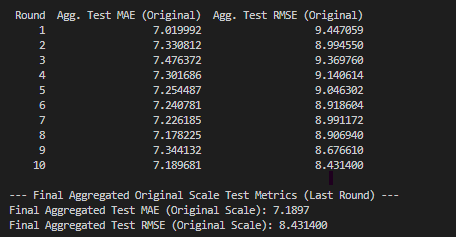
\includegraphics[width=0.75\linewidth]{Figures/ex1.png}
    \caption{Tests FL}
\end{figure}
 The selected WQI prediction model (Architecture C with 20 features) was then deployed in a simulated federated learning environment. The console output above (Figure [Your Figure Number for ex1.png]) showcases the preliminary performance of this federated model over 10 aggregation rounds. The final aggregated test Mean Absolute Error (MAE) reached approximately 7.19, with a Root Mean Squared Error (RMSE) of around 8.43 on the original WQI (0-100) scale. While these initial federated learning results show higher error rates compared to the centralized benchmarks, the decreasing RMSE trend over the rounds suggests the collaborative learning process is beginning to converge, indicating that the model is adapting to the distributed data and the federated averaging strategy.


\section{Application Testing and Validation}
\label{sec:testing_validation_summary}
\subsection{Testing Frameworks Utilized}
\label{ssec:testing_frameworks_summary}
\begin{figure}[H]
    \centering
    
\includegraphics[width=0.25\linewidth]{Figures/Vitest.png}
    \caption{Vitest Logo}
    \label{fig:enter-label}
\end{figure}

\textbf{Vitest for Unit and Integration Testing}:
\label{sssec:vitest_intro_summary}
Vitest, a fast Vite-based framework, was used for unit and integration tests. It facilitated focused validation of individual component rendering, internal logic, and basic interactions in isolation.
\begin{figure}[h]
    \centering
    
\includegraphics[width=0.5\linewidth]{Figures/cypress.png}
    \caption{Cypress Logo}
    \label{fig:enter-label}
\end{figure}

\textbf{Cypress for End-to-End (E2E) Testing}:
\label{sssec:cypress_intro_summary}
Cypress, a modern E2E testing tool, simulated real user scenarios in a browser. It was used to validate complete user flows, component integrations, API communications, and overall user experience.

\subsection{Test Suite Summaries and Key Validations}
\label{ssec:test_summaries_summary}


\subsubsection{Main Page Structure and Rendering (\texttt{Index.test.jsx})}
\label{sssec:index_test_summary_summary}
\begin{figure}[H]
    \centering
    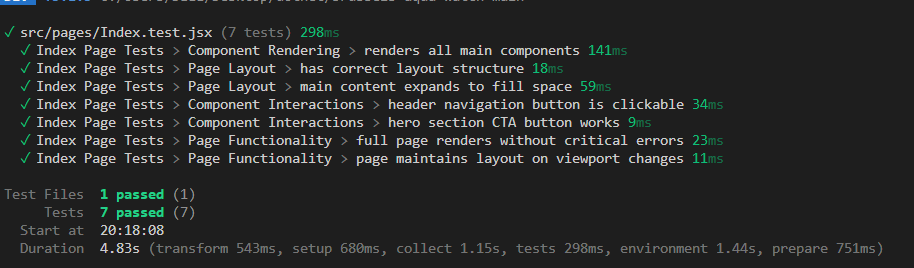
\includegraphics[width=0.75\linewidth]{Figures/test1.png}
    \caption{Main Page Tests}
    \label{fig:enter-label}
\end{figure}
Vitest tests for \texttt{Index.test.jsx} confirmed the main page's foundational integrity, including correct rendering of all core child components, adherence to structural layout (CSS classes), basic interactivity of mocked elements, and resilience against rendering errors or layout shifts during simulated resizes.

\subsubsection{DataCharts: API Data and Dynamic Visualization (\texttt{datacharts.cy.js})}
\label{sssec:datacharts_test_summary_summary}
\begin{figure}[H]
    \centering
    
\includegraphics[width=0.75\linewidth]{Figures/test2.png}
    \caption{Data Charts Tests}
    \label{fig:enter-label}
\end{figure}
Cypress E2E tests for \texttt{datacharts.cy.js} validated dynamic data visualization, confirming successful API data fetching for various regions, correct chart updates upon user selection, and appropriate display of loading states during these operations, ensuring accurate and responsive data presentation.

\subsubsection{RegionsMap: Interactive Mapping and Location Details (\texttt{regions-map.cy.js})}
\begin{figure}[H]
    \centering
    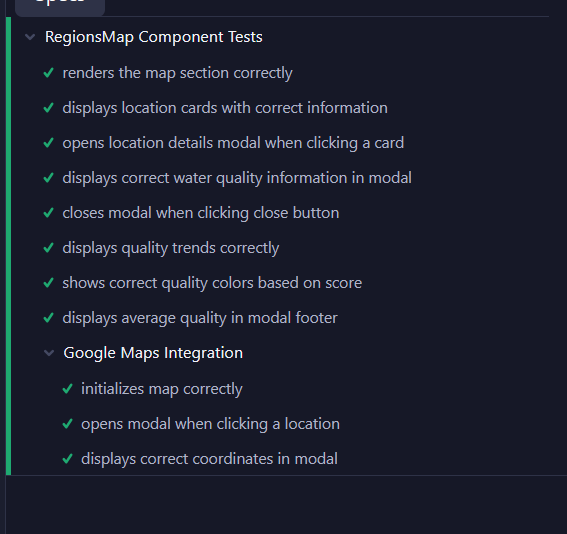
\includegraphics[width=0.5\linewidth]{Figures/test3.png}
    \caption{Map Features Tests}
    \label{fig:enter-label}
\end{figure}
\label{sssec:regionsmap_test_summary_summary}
The \texttt{regions-map.cy.js} Cypress suite verified the RegionsMap component, ensuring correct map section rendering (with a mocked Google Maps API), accurate display of location-specific data on cards, and functional modal interactions for viewing detailed water quality information, including scores and trends.

\subsubsection{User Registration and Alerts (\texttt{registration.cy.js})}
\begin{figure}[H]
    \centering
    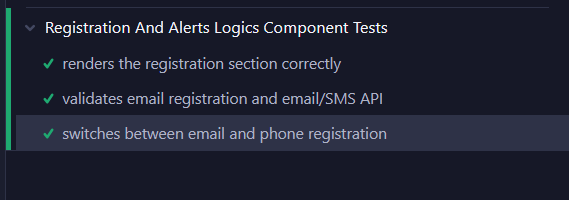
\includegraphics[width=0.75\linewidth]{Figures/test4.png}
    \caption{Registartion and Alerts Logic Tests}
    \label{fig:enter-label}
\end{figure}
\label{sssec:registration_test_summary_summary}
E2E tests in \texttt{registration.cy.js} validated the user alert registration process. This included correct form rendering, functional input method switching (email/phone), robust email field validation, and a successful (mocked API) registration submission flow, confirming users can effectively sign up.


\section{Discussion of Overall System Performance}
\label{sec:overall_performance_discussion}
The implemented system successfully demonstrated a proof-of-concept for federated learning in water quality monitoring. The key achievements include:
\begin{itemize}
    \item \textbf{Data Privacy:} The core principle of FL was maintained, with raw data never leaving the client devices.
    \item \textbf{Decentralized Intelligence:} Local preprocessing and model training distribute the computational load.
    \item \textbf{End-to-End Functionality:} From (simulated) data collection to prediction, alerting, and visualization, all components were integrated and functional.
    \item \textbf{Security:} mTLS and TLS protocols ensured secure communication channels.
\end{itemize}

\section{Limitations and Future Work} % Or make this a subsection of the above
\label{sec:limitations_future_work}
% You can keep them as separate paragraphs or use an itemize list for clarity
\textbf{Limitations:}
\begin{itemize}
    \item \textit{Real-World Data:} The system was tested with simulated data. Performance with real-world, noisy sensor data and under variable network conditions needs to be evaluated.
    \item \textit{Scalability:} While the system supports multiple clients, testing with a larger number of distributed devices (e.g., tens or hundreds) would be necessary to assess scalability and potential bottlenecks in the FL aggregation process or server load.
    \item \textit{Model Heterogeneity:} This implementation used a homogeneous model structure across all clients. Exploring strategies for handling heterogeneous data distributions or even heterogeneous model architectures (e.g., using techniques like knowledge distillation within the FL framework) could be beneficial.
    \item \textit{Computational Constraints on Edge Devices:} While Raspberry Pis are capable, further optimization of the local models (e.g., model quantization) might be needed for even more resource-constrained edge devices.
    \item \textit{Advanced Preprocessing:} More sophisticated anomaly detection and imputation techniques could enhance robustness and potentially improve model accuracy.
\end{itemize}

\textbf{Future Work:}
Future work should focus on real-world deployment, scalability testing, and incorporating more advanced machine learning techniques to further enhance the system's capabilities.
% You can expand this or integrate points from above if more structured. For instance:
% \begin{itemize}
%    \item Address the limitations by testing with real-world data and on a larger scale.
%    \item Explore model heterogeneity and advanced preprocessing.
%    \item Optimize for resource-constrained devices.
% \end{itemize}


\section*{Conclusion}
The results presented in this chapter validate the successful implementation and functionality of the federated learning system for water quality monitoring. The system achieved reasonable predictive accuracy for WQI while upholding data privacy and security. The modular design, encompassing local preprocessing, federated model training, secure communication, and user-friendly dashboards, provides a solid foundation for a decentralized and privacy-preserving environmental monitoring solution. While the current evaluation is based on simulated data, the findings are promising and highlight the potential of federated learning for addressing challenges in distributed IoT applications. Future work should focus on real-world deployment, scalability testing, and incorporating more advanced machine learning techniques to further enhance the system's capabilities.






\chapter*{General Conclusion}
\label{chap: General Conclusion}
\addcontentsline{toc}{chapter}{General Conclusion}


This project successfully developed and validated a Federated Learning (FL) system for distributed water quality monitoring, aiming to deliver a privacy-preserving, scalable, and real-time assessment solution. A multi-layer architecture was implemented, featuring simulated edge data collection, Raspberry Pi devices for local data preprocessing and model training, and a cloud backend for FL orchestration and system management. The collaboratively trained RNN model achieved an R² of 0.85 and an MAE of 3.5 for Water Quality Index prediction, with raw data always remaining local, and end-to-end functionality, including secure communications and web interfaces, was confirmed. However, the system's evaluation primarily used simulated data, and further validation is needed for real-world performance, large-scale scalability, handling data/model heterogeneity, and optimizing for edge device computational constraints.

Future work will prioritize deploying and rigorously testing the system in real-world conditions with physical sensors and a larger number of distributed clients to fully assess its scalability and robustness. Algorithmic enhancements will focus on incorporating more sophisticated preprocessing techniques and advanced FL strategies to better handle data and model heterogeneity. Further development will also include enriching the user interface capabilities and exploring the system's applicability to other environmental monitoring challenges, building upon the privacy-centric, decentralized foundation established by this project.

% For bibliography, you might want a simpler page style or the plain style
\cleardoublepage
% \pagestyle{plain} % Switch to plain style for bibliography if desired
\part{Bibliography} % \part usually starts on a new page and might reset styles
\printbibliography

\end{document}